\documentclass[12pt]{article}
\usepackage[T1]{fontenc}
\usepackage{lmodern}
\usepackage{amsmath,amssymb,amsthm,mathtools}
\usepackage[letterpaper,margin=1.1in]{geometry}
\usepackage{enumitem,booktabs,longtable,array}
\usepackage{xcolor}
\usepackage{tikz-cd}
\usetikzlibrary{positioning,calc}
\usepackage[colorlinks=true,linkcolor=blue!50!black,citecolor=blue!50!black,urlcolor=blue!50!black]{hyperref}

% ---------------- notation (as in [JC], plus additions) ----------------
\newcommand{\ov}[1]{\overline{#1}}
\newcommand{\eps}{\epsilon}
\newcommand{\A}{\mathbb{A}}
\newcommand{\C}{\mathbb{C}}
\newcommand{\Q}{\mathbb{Q}}
\newcommand{\Z}{\mathbb{Z}}
\newcommand{\cO}{\mathcal{O}}
\newcommand{\gen}{\mathrm{gen}}
\newcommand{\reg}{\mathrm{reg}}
\newcommand{\tr}{\operatorname{tr}}
\newcommand{\Gal}{\operatorname{Gal}}
\newcommand{\Aut}{\operatorname{Aut}}
\newcommand{\Nrd}{\operatorname{Nrd}}
\newcommand{\Ad}{\operatorname{Ad}}
\newcommand{\Hom}{\operatorname{Hom}}
\newcommand{\Iso}{\operatorname{Iso}}
\newcommand{\vol}{\operatorname{vol}}
\newcommand{\supp}{\operatorname{supp}}
\newcommand{\diag}{\operatorname{diag}}
\newcommand{\GL}{\mathrm{GL}}
\newcommand{\SL}{\mathrm{SL}}
\newcommand{\Gb}{\ov{G}}
\newcommand{\Zb}{\ov{Z}}
\newcommand{\GDb}{\ov{G}_D}
\newcommand{\pib}{\ov{\pi}}
\newcommand{\ks}{\kappa^{*}}
\newcommand{\Eb}{\ov{E}}
\newcommand{\Tb}{\ov{T}}
\newcommand{\cG}{\mathcal{G}}
\newcommand{\cGb}{\ov{\mathcal{G}}}
\newcommand{\iD}{\iota_D}
\newcommand{\iG}{\iota_{\GL}}
\newcommand{\jj}{\jmath}
\newcommand{\Pv}{\textbf{[P]}}
\newcommand{\Ev}{\textbf{[E]}}
\newcommand{\Ov}{\textbf{[O]}}
\newcommand{\Cv}{\textbf{[C]}}

\theoremstyle{plain}
\newtheorem{theorem}{Theorem}[section]
\newtheorem{proposition}[theorem]{Proposition}
\newtheorem{lemma}[theorem]{Lemma}
\newtheorem{corollary}[theorem]{Corollary}
\newtheorem{conjecture}[theorem]{Conjecture}
\theoremstyle{definition}
\newtheorem{definition}[theorem]{Definition}
\newtheorem{remark}[theorem]{Remark}
\newtheorem{example}[theorem]{Example}
\newtheorem{assumption}[theorem]{Standing assumptions}

\title{A metaplectic Jacquet--Langlands transfer for division algebras of prime degree, I:\\ local matching and a global transfer under elliptic-support conditions\\[0.4em]\normalsize Draft 9}
\author{David Joyner \and Claude (Anthropic) \and ChatGPT (OpenAI)}
\date{November 8, 2026}

\emergencystretch=3em
\begin{document}
\maketitle

\begin{abstract}
Let $D$ be a central division algebra of prime degree $r$ over a totally imaginary number field $K$ containing $\mu_n$, with $n$ odd and $(n,r)=1$. We compare the $n$-fold cover of $D^\times_{\A}$ constructed in [JC] with the Kazhdan--Patterson cover of $\GL(r,\A_K)$, realizing both as subgroups of one cover of $\GL(r,\A_L)$, where $L\subset D$ is a cyclic maximal subfield. \emph{Theorem~A:} at each ramified place of $D$, the covered elliptic tori on the two sides have the same commutator pairing and the same good elements, and they are identified on good elements by a canonical isomorphism. \emph{Theorem~B:} genuine test functions supported on the regular set have matching functions on the other side, in both directions. \emph{Theorem~C:} using a variant of the simple trace formula of Flicker--Kazhdan, we prove a locally finite identity of packets at the ramified places. From it we obtain a cuspidal transfer, with the same components away from the ramified places, for every genuine automorphic representation of the cover of $D^\times_{\A}$ that has a supercuspidal component at some split place, under a non-cancellation hypothesis that holds whenever the $D$-side packet is finite. Part~II proves the matching of arbitrary functions and replaces this hypothesis by a weaker one; Part~III studies the local character relations from the side of the division algebra.
\end{abstract}

\tableofcontents

% =====================================================================
\section{Introduction}\label{sec:intro}
This section states the main results, fixes the standing assumptions and conventions, explains how results are labeled, and describes what the later parts of the series do. It depends on nothing else in the paper. The global data $K,n,r,L,D,S,r',c,c_v$ are fixed in Assumption~\ref{ass:standing}; all notation, including the status labels and the cocycle normalization, is collected in \S\ref{sec:glossary}, and the results are summarized, with labels and pointers, in the \hyperref[sec:summary]{Summary of results} that follows this section. Throughout, [JC] refers to the corrected version (\texttt{metaplectic\_kazhdan\_revised12.tex}) of [J], and a reference such as [JC, Lemma~6.1] is to the numbering there.

\subsection{Setting and aim}
We fix the global data, which are those of [JC, \S1], and explain where this paper fits.

\begin{assumption}\label{ass:standing}
$K$ is a totally imaginary number field containing $\mu_n$, with $n\ge1$ odd; $L/K$ is cyclic of prime degree $r$ with $(n,r)=1$; $D$ is a central division algebra over $K$ of dimension $r^2$ containing $L$; and $S$ is the set of places where $D$ ramifies. Fix $r'\in\Z$ with $rr'\equiv1\pmod n$ and $c\in\Z$ with $n\mid r-1+2c$, and put $c_v:=r'c$, so that $n\mid r-1+2rc_v$.
\end{assumption}

The paper [JC] lifts genuine automorphic representations of an $n$-fold cover of the torus $L^\times_{\A}$ to $\eps$-invariant genuine automorphic representations of an $n$-fold cover $\GDb(\A_K)$ of $D^\times_{\A}$. Its Remark~10.3 outlines the missing step needed to reach the Kazhdan--Patterson cover $\Gb(\A_K)$ of $\GL(r,\A_K)$: a metaplectic Jacquet--Langlands transfer from $\GDb$ to $\Gb$. Part~I (this paper) establishes the local matching of test functions that the transfer requires, and a global transfer for representations with suitable local components. The later parts of the series (\S\ref{subsec:partII}) remove some of those conditions and study the local character relations.

Since $r$ is prime, every $v\in S$ is finite (the archimedean places are complex), $D_v$ is a division algebra, and $L_v:=L\otimes_KK_v$ is a field. The local invariants of $D$ are nonzero elements of $\frac1r\Z/\Z$ with sum $0$, so $|S|\ge2$, and $|S|$ is even if $r=2$.

\subsection{Main results}\label{subsec:mainresults}
We state the three main results informally; precise statements are referenced.

\emph{Covers.} Both $\GDb(\A_K)$ and $\Gb(\A_K)$ are realized as subgroups of one cover of $\GL(r,\A_L)$ (\S\ref{sec:covers}, \S\ref{sec:global}), so that their centers, rational splittings and central characters are literally shared.

\paragraph{Theorem A (covered tori; Theorem~\ref{thm:ident}).} Let $v\in S$, let $E\subset D_v$ be a maximal subfield, and embed $E$ in $M_r(K_v)$. The covered tori $\Eb_D\subset\GDb(K_v)$ and $\Eb_{\GL}\subset\Gb(K_v)$ have the same commutator pairing $(x,y)\mapsto((Nx)^{1+2c_v}x^{-1},y)_E$. Their good elements are the inverse image of $K_v^\times E^{\times n}$, of index $|n|_{K_v}^{-(r-1)}$. There is an isomorphism $\Eb_D\cong\Eb_{\GL}$ induced by conjugation in the ambient cover, and its restriction to the good elements is canonical: it is the same for every isomorphism that is the identity on the common center.

\paragraph{Theorem B (local matching; Theorem~\ref{thm:easy}).} With matching defined by $F(\tilde\gamma,\tilde f_D)=(-1)^{r-1}F(\jj(\tilde\gamma),\tilde f)$ at good regular elements, and vanishing of the $\GL$-side orbital integrals at non-elliptic elements, every genuine $\tilde f_D$ on $\GDb(K_v)$ vanishing near the center has a matching $\tilde f$ supported on the good regular elliptic set of $\Gb(K_v)$. Conversely, every regular-supported $\tilde f$ with vanishing non-elliptic orbital integrals has a matching $\tilde f_D$. For general $\tilde f_D$ the method necessarily fails (Proposition~\ref{prop:germ}), and germ expansions are needed.

\paragraph{Theorem C (global transfer; Proposition~\ref{prop:packet}, Theorems~\ref{thm:transfer} and~\ref{thm:converse}).} Let $\pib_D$ be a genuine automorphic representation of $\GDb(\A_K)$ whose component at some finite place $w_0\notin S$ is supercuspidal. Let $P_D\ni\pib_D$ and $P$ be the packets of $D$-side and cuspidal $\GL$-side representations with the same components outside $S$. These packets satisfy an identity of traces at the places of $S$ against all matching regular-supported test functions; the sums are locally finite. If the $D$-side packet is \emph{not cancelled} on regular-supported test functions (hypothesis $(\mathrm H_D)$, which holds whenever $P_D$ is finite), then there is a genuine cuspidal automorphic representation $\pib$ of $\Gb(\A_K)$ with $\pib_v\cong\pib_{D,v}$ for all $v\notin S$. A converse holds under the analogous hypothesis (H) on the $\GL$-side packet. Lemma~\ref{lem:cancel} shows that $(\mathrm H_D)$ can fail only if, at every level, the coefficient function of the packet at $S$ lies in the sum of the subspaces having a Plancherel factor at one place of $S$.

Theorem~C rests on the simple trace formula of Flicker and Kazhdan [FK, \S18]. We need it in a slightly different form, with the supercusp form at a place outside $S$; this variant is proved in Proposition~\ref{prop:FKvariant}. Since the multiplicity-one and local character theory needed to isolate single representations is not available here, Theorem~C is a statement about packets.

\subsection{Goals of the later parts}\label{subsec:partII}
The goals below are needed to complete the metaplectic Jacquet--Langlands correspondence by removing the restrictions of Theorems~B and~C. Each item lists the inputs it needs, followed by its current status in the later parts of the series. References to Part~II are to Draft~8 and those to Part~III are to Draft~9.
\begin{enumerate}[label=(\roman*)]
\item \emph{Matching of arbitrary functions.} Extend Theorem~B to all $\tilde f_D$, and to all $\tilde f$ with vanishing non-elliptic orbital integrals. This needs the germ expansions of [FK, \S8] at central good elements, their restriction to the elliptic set, and a genuine function with the orbital integrals of a Steinberg pseudo-coefficient near the center, and an analog of [DKV, A.3] (\S\ref{subsec:general}, item (D1)). \emph{Status:} proved in Part~II (Theorem~E).
\item \emph{Local character relations.} Prove a metaplectic local Jacquet--Langlands correspondence: a bijection $\pib_v\leftrightarrow\pib_{D,v}$ between genuine square-integrable representations of $\Gb(K_v)$ and genuine irreducible representations of $\GDb(K_v)$, with $\Theta_{\pib_{D,v}}=(-1)^{r-1}\Theta_{\pib_v}\circ\jj$ on good regular elements (item (D2)). This needs (i), the elliptic orthogonality relations of [FK, \S\S24--25], and multiplicity one and rigidity for $\Gb(\A_K)$ ([FK, \S\S27--28], as corrected in [Z]). \emph{Status:} Part~III constructs a unitary transform $L_D$ between ordinary and genuine invariant class functions on $D_v^\times$ and its cover, and proves that it bijects irreducible characters at the places $v\in S$ of residue characteristic prime to $n$. When the square-integrable Flicker--Kazhdan correspondence is available in Zou's corrected form [Z, Proposition~3.6, Definition~3.7], Part~III, Corollary~7.8, proves (D2) at such tame places; the published sufficient range $(n,N_r)=1$ and the precise compatibility checks are recorded in Remark~\ref{rem:D2tame}. Outside that range an appropriate metaplectic correspondence theorem is an additional input. At places dividing $n$ the irreducible-character integrality needed for this composition remains open.
\item \emph{An unconditional global correspondence.} Remove the auxiliary supercuspidal place in Theorem~C, either via W.-W.~Li's trace formula for covers [Li4] or via (i), and refine the packet identity of Theorem~C to a correspondence of individual representations using (ii). \emph{Status:} open; see Part~II, \S7(iii).
\item \emph{Removing $(\mathrm H_D)$ and (H).} Prove finiteness of near-equivalence packets for $\GDb(\A_K)$ (for example, by bounding the level at $S$ in terms of the components outside $S$), and linear independence of elliptic characters in $\GL$-side packets, so that Theorem~C becomes unconditional (Remark~\ref{rem:H}, item (D3)). \emph{Status:} Part~II replaces $(\mathrm H_D)$ by the weaker $(\mathrm H_D')$ and reduces its removal to a bound on levels at $S$ (Part~II, Corollary~6.11); open in general.
\item \emph{Completing [JC, Remark~10.3].} Compose the lifting of [JC] with the transfer, to obtain genuine automorphic representations of the Kazhdan--Patterson cover of $\GL(r,\A_K)$ attached to genuine characters of the covered torus (item (D4)). Then compare the result with the Flicker--Kazhdan correspondence [FK] to $\GL(r,\A_K)$ and with Kazhdan's endoscopic lifting. \emph{Status:} open.
\end{enumerate}

\subsection{Conventions}
The conventions below are repeated, with the rest of the series' notation, in \S\ref{sec:glossary} (Hilbert symbols in \S\ref{gl:hilbert}, covers and the relabeling of $\mu_n$ in \S\ref{gl:cocycle}, genuine objects and good elements in \S\ref{gl:genuine}).

All Hilbert symbols are $n$-th Hilbert symbols. For a finite extension $F'/F$ of local fields containing $\mu_n$, $a\in F^\times$ and $b\in F'^\times$, we use the norm compatibility $(a,b)_{F'}=(a,N_{F'/F}b)_F$ [Ser, Ch.~XIV]; in particular $(a,b)_{F'}=(a,b)_F^{[F':F]}$ for $a,b\in F^\times$. For lifts $\tilde x,\tilde y$ of commuting elements, $[x,y]=\tilde x\tilde y\tilde x^{-1}\tilde y^{-1}$. For a cover $p:\ov H\to H$ and $H'\subset H$ we write $\ov{H'}=p^{-1}(H')$. Genuine functions and representations, good elements, and $C_c^\infty(\ov H,\tilde\theta)_\gen$ are as in [JC, \S\S1--2]. As in [JC, \S6.1], we relabel $\mu_n$ once, by $\zeta\mapsto\zeta^{r'}$, at every place and globally, and we say explicitly when a formula is stated before or after relabeling.

\subsection{How results are labeled}
The labels are those of the whole series (\S\ref{gl:labels}, which also defines the label \textbf{[P$^{\mathrm c}$]} used in the companion paper; it does not occur here). Statements are marked by status:
\begin{itemize}
\item \Pv\ \emph{Proved here}: a complete argument is included, possibly using cited results marked \Ev.
\item \Ev\ \emph{Established elsewhere}: a precisely cited theorem, used as a black box.
\item \Ov\ \emph{Proof outlined}: the steps are identified, but at least one remains to be written out or checked.
\item \Cv\ \emph{Conjectural}: requires new mathematical input (later parts of the series).
\end{itemize}

\begin{center}
\begin{tabular}{>{\raggedright\arraybackslash}p{0.47\textwidth}>{\raggedright\arraybackslash}p{0.15\textwidth}>{\raggedright\arraybackslash}p{0.25\textwidth}}
\toprule
Statement & Where & Status\\
\midrule
Both covers are subgroups of one ambient cover; the $\GL$ side is the Kazhdan--Patterson cover with parameter $c_v$ & Prop.~\ref{prop:restriction} & \Pv\\
Section and splitting conventions & Lemma~\ref{lem:splittings} & \Pv\\
Canonical identification of the covers at $v\notin S$ & Prop.~\ref{prop:outsideS} & \Pv\\
Covered elliptic tori at $v\in S$: pairings, good elements, centers; canonical identification (Theorem~A) & \S\ref{sec:tori} & \Pv\\
Matching for regular-supported functions (Theorem~B) & Thm.~\ref{thm:easy}, App.~\ref{app:oi} & \Pv\\
Global covers; rational lifts correspond & \S\ref{sec:global} & \Pv\\
Geometric expansions, including class-counting constants & Props.~\ref{prop:geomD}, \ref{prop:FKvariant} & \Pv\\
Variant of the simple trace formula of [FK, \S18] & Prop.~\ref{prop:FKvariant} & \Pv\\
Comparison of the trace formulas & Thm.~\ref{thm:comparison} & \Pv\\
Packet identity at $S$ (locally finite) & Prop.~\ref{prop:packet} & \Pv\\
Characterization of cancellation & Lemma~\ref{lem:cancel} & \Pv\\
Global transfer (Theorem~C) & Thm.~\ref{thm:transfer} & \Pv\ under $(\mathrm H_D)$; unconditional for finite packets\\
Converse transfer & Thm.~\ref{thm:converse} & \Pv\ under (H)\\
Finiteness of packets; removal of $(\mathrm H_D)$, (H) & \S\ref{sec:deferred} & \Cv\ (weakened in Part~II)\\
Matching of arbitrary functions; local character relations & \S\ref{sec:deferred} & \Cv\ (matching: Part~II; tame character relations with FK--Zou input: Part~III)\\
\bottomrule
\end{tabular}
\end{center}

The logical dependencies are as follows. Arrows mean ``is used in'', and the notes on the right list the additional inputs of each step.
\begin{center}
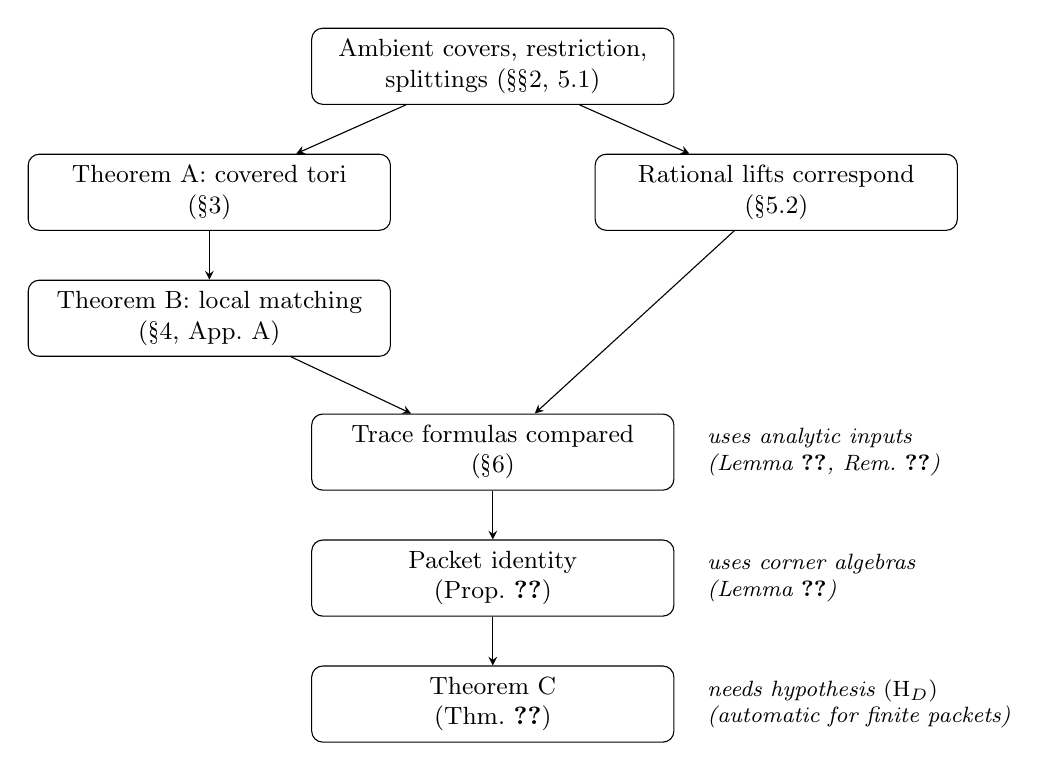
\begin{tikzpicture}[box/.style={draw,rounded corners,align=center,font=\small,inner sep=4pt,minimum width=4.6cm},ann/.style={font=\footnotesize\itshape,align=left,anchor=west},>=stealth]
\node[box] (cov) at (0,0) {Ambient covers, restriction,\\ splittings (\S\S2, 5.1)};
\node[box] (A) at (-3.6,-1.6) {Theorem A: covered tori\\ (\S3)};
\node[box] (rat) at (3.6,-1.6) {Rational lifts correspond\\ (\S5.2)};
\node[box] (B) at (-3.6,-3.2) {Theorem B: local matching\\ (\S4, App.~A)};
\node[box] (TF) at (0,-4.9) {Trace formulas compared\\ (\S6)};
\node[box] (P) at (0,-6.5) {Packet identity\\ (Prop.~\ref{prop:packet})};
\node[box] (C) at (0,-8.1) {Theorem C\\ (Thm.~\ref{thm:transfer})};
\draw[->] (cov)--(A); \draw[->] (cov)--(rat); \draw[->] (A)--(B);
\draw[->] (B)--(TF); \draw[->] (rat)--(TF); \draw[->] (TF)--(P); \draw[->] (P)--(C);
\node[ann] at (2.6,-4.9) {uses analytic inputs\\ (Lemma~\ref{lem:A1}, Rem.~\ref{rem:Einputs})};
\node[ann] at (2.6,-6.5) {uses corner algebras\\ (Lemma~\ref{lem:corner})};
\node[ann] at (2.6,-8.1) {needs hypothesis $(\mathrm H_D)$\\ (automatic for finite packets)};
\end{tikzpicture}
\end{center}
Everything except the last box is unconditional, given the cited \Ev\ inputs. The \Ev\ inputs used in the global sections are listed in Remark~\ref{rem:Einputs}.

\subsection*{A running example}
Throughout the series we test the constructions on one case: $K=\mathbb{Q}(\zeta_3)$, $n=3$, $r=2$, $D=(-1,4-\zeta_3)_K$, which is ramified exactly at $S=\{\mathfrak p_3,\mathfrak p_7\}$, with $\mathfrak p_3=(1-\zeta_3)$ and $\mathfrak p_7=(3+\zeta_3)$. We take $L=K(i)=\mathbb{Q}(\zeta_{12})$, and $c=1$, $r'=2$, $c_v=2$ in Assumption~\ref{ass:standing}. At $\mathfrak p_3$, where $K_v=\mathbb{Q}_3(\zeta_3)$, the covered elliptic tori are non-abelian: the good elements have index $9$, and genuine irreducibles of a covered torus have dimension $3$ (Example~\ref{ex:r2n3}). At $\mathfrak p_7$, where $K_v=\mathbb{Q}_7\supset\mu_3$, they are abelian. The sign in Theorem~\ref{thm:easy} is $-1$. The note \texttt{notes/mjl\_running\_example.tex} in the project repository works this case out across Parts~I--IV.

\subsection{Organization}
Sections~\ref{sec:covers}--\ref{sec:matching}, together with Appendix~\ref{app:oi}, contain the local theory. Sections~\ref{sec:global}--\ref{sec:spectral} contain the global theory, and Appendix~\ref{app:cusp} supplies their analytic input for cusp forms on the cover. Section~\ref{sec:deferred} lists what is left after this paper, and Section~\ref{sec:conclusion} summarizes what the local theory gives on its own. Section~\ref{sec:glossary} collects the notation and conventions of the series (shared by all four Parts) together with the notation specific to Part~I, and Section~\ref{sec:lit} reviews the literature for the whole series; Parts~II--IV refer to it. The \hyperref[sec:summary]{Summary of results} after this section lists the results with their labels.


% =====================================================================
\section*{Summary of results}\addcontentsline{toc}{section}{Summary of results}\label{sec:summary}
The results of Part~I, with status labels (\S\ref{gl:labels}) and pointers; notation as in Assumption~\ref{ass:standing} and \S\ref{sec:glossary}, with $v\in S$ and $F=K_v$.

\begin{enumerate}[leftmargin=*,label=\arabic*.]
\item \textbf{One ambient cover} (Lemma~\ref{lem:center}, Proposition~\ref{prop:restriction}; \Pv\ using \Ev). The cover $\GDb(K_v)$ of [JC] and the Kazhdan--Patterson cover $\Gb_v$ of $\GL(r,K_v)$ are subgroups of one cover $\cGb_v$ of $\GL(r,L_v)$, with the same central subgroup $\Zb_v$. As an extension, $\Gb_v$ is the parameter-$c_v$ cover after relabeling $\mu_n$, and the parameter is forced (Remark~\ref{rem:forced}). At $v\notin S$ they are identified canonically by conjugation (Proposition~\ref{prop:outsideS}; \Pv).
\item \textbf{Theorem~A: covered elliptic tori} (Proposition~\ref{prop:comm}, Proposition~\ref{prop:good}, Theorem~\ref{thm:ident}, Corollaries~\ref{cor:classes} and~\ref{cor:reps}; \Pv). For every maximal subfield $E\subset D_v$ the two covered tori have the commutator pairing $((Nx)^{1+2c_v}x^{-1},y)_E$ and the good elements $p^{-1}(F^\times E^{\times n})$, of index $|n|_F^{-(r-1)}$. Every isomorphism between them over $\iG\circ j\circ\iD^{-1}$ that is the identity on $\Zb_v$ has the same restriction $\jj_{E,j}$ to the good elements. This gives a canonical bijection $\jj$ of good regular elliptic classes and of genuine representations of covered tori.
\item \textbf{Theorem~B: matching on the regular set} (Theorem~\ref{thm:easy}, Appendix~\ref{app:oi}; \Pv). Matching (Definition~\ref{def:matching}) carries the sign $(-1)^{r-1}$. Every genuine $\tilde f_D$ vanishing near $\Zb_v$ has a matching $\tilde f$ supported on the good regular elliptic set, and conversely every regular-supported $\tilde f$ with vanishing non-elliptic orbital integrals has a matching $\tilde f_D$. Near the center the method fails (Proposition~\ref{prop:germ}; \Pv).
\item \textbf{Rational elements and trace formulas} (Theorem~\ref{thm:rational}, Corollary~\ref{cor:rationalbij}, Propositions~\ref{prop:geomD} and~\ref{prop:FKvariant}, Theorem~\ref{thm:comparison}; \Pv\ using the \Ev\ inputs of Remark~\ref{rem:Einputs}). The elliptic terms of the two trace formulas agree term by term; on the $\GL$ side we use a variant of [FK, \S18] with the supercusp form at a place $w_0\notin S$.
\item \textbf{Packet identity} (Proposition~\ref{prop:packet}; \Pv, unconditional). The $D$-side and cuspidal $\GL$-side near-equivalence packets with the same components outside $S\cup\{w_0\}$ have equal traces at $S$ against matching regular-supported test functions; both sums are locally finite.
\item \textbf{Theorem~C: global transfer} (Theorem~\ref{thm:transfer}; \Pv\ under $(\mathrm H_D)$). A genuine automorphic $\pib_D$ with a supercuspidal component at some finite $w_0\notin S$ transfers to a genuine cuspidal $\pib$ with the same components outside $S$, if its packet satisfies $(\mathrm H_D)$; this holds when the packet is finite (Proposition~\ref{prop:HDfinite}; \Pv). The converse holds under (H) (Theorem~\ref{thm:converse}), and Lemma~\ref{lem:cancel} (\Pv) shows exactly how $(\mathrm H_D)$ could fail.
\item \textbf{What is left} (\S\ref{sec:deferred}; \Cv). (D1) matching of arbitrary functions, (D2) local character relations, (D3) finiteness of packets, (D4) composition with [JC]. Part~II proves (D1), and Part~III proves (D2) at tame places in the range of the corrected Flicker--Kazhdan correspondence (Remark~\ref{rem:D2tame}); the rest is open.
\end{enumerate}
\emph{Running example} (Example~\ref{ex:r2n3}): the covered elliptic tori are non-abelian at $\mathfrak p_3$ (index $9$, dimension $3$) and abelian at $\mathfrak p_7$; the sign in Theorem~B is $-1$.

% =====================================================================
\section{Local covers}\label{sec:covers}
This section realizes the cover of $D_v^\times$ from [JC] and the Kazhdan--Patterson cover of $\GL(r,K_v)$ as subgroups of one cover of the larger group $\GL(r,L\otimes_KK_v)$ (\S\ref{subsec:why}--\ref{subsec:ambient}). It then shows that the $\GL$-side subgroup is the Kazhdan--Patterson cover with parameter $c_v$, as an extension (\S\ref{subsec:restriction}), and identifies the two covers canonically at the places where $D$ splits (\S\ref{subsec:outsideS}). It depends only on the Kazhdan--Patterson cocycle [KP1, \S0.1], [FK, \S2] and the Matsumoto--Moore classification [Mat], [Moo], and uses from [JC] only the definition of the cover of $D_v^\times$. It introduces the ambient cover $\cGb_v$, the embeddings $\iD$ and $\iG$, the local covers $\GDb(K_v)$ and $\Gb_v$, their common central subgroup $\Zb_v$, and the identifications $\psi_v$ at $v\notin S$.

\subsection{Why an ambient cover}\label{subsec:why}
We explain the idea before the computations.

Equality of commutator pairings does not, by itself, give a preferred isomorphism between two central extensions. Any two isomorphisms differ by a character with values in $\mu_n$, and such characters can be nontrivial on the center. A careless choice would therefore make the comparison of central characters, and hence of genuine functions, ambiguous. Our approach is to realize both covers as \emph{subgroups} of a single cover of $\GL(r,L\otimes_KK_v)$. Conjugation in this larger group then produces isomorphisms between the relevant subgroups. These isomorphisms are in general not unique, but their restrictions to the centers of covered tori are canonical (Theorem~\ref{thm:ident}). Because both covers sit in one group, the common central subgroup $p^{-1}(K_v^\times)$ is literally the same subgroup on the two sides. This uses no choice of cocycle, so the question of whether two cocycles agree exactly or only up to a coboundary does not arise for it.

\subsection{The ambient cover}\label{subsec:ambient}
We define the ambient cover at each place and the two subgroups; the notation $\cGb_v$, $\iD$, $\iG$, $\GDb(K_v)$, $\Gb_v$, $\Zb_v$ introduced here is used throughout.

Fix once and for all an isomorphism $D\otimes_KL\cong M_r(L)$. For a place $v$ of $K$ put $L_v=L\otimes_KK_v=\prod_{w\mid v}L_w$ and $\cG_v:=\GL(r,L_v)=\prod_{w\mid v}\GL(r,L_w)$. Let $\cGb_v$ be the cover of $\cG_v$ obtained from the product of the Kazhdan--Patterson covers of the $\GL(r,L_w)$ with twisting parameter $c_v$, by identifying their copies of $\mu_n$ (i.e.\ the quotient of the product by $\{(\zeta_w):\prod_w\zeta_w=1\}$). A cocycle for $\cGb_v$ is
\begin{equation}\label{eq:ambient}
\prod_{w\mid v}\sigma_{L_w}(g_w,h_w)\,(\det g_w,\det h_w)_{L_w}^{c_v},
\end{equation}
where $\sigma_{L_w}$ is the Kazhdan--Patterson cocycle with parameter $0$ [KP1, \S0.1], [FK, \S2]. Let
\[ \iD:D_v^\times\hookrightarrow\cG_v,\qquad \iG:\GL(r,K_v)\hookrightarrow\cG_v \]
be the embedding induced by $D\otimes_KL\cong M_r(L)$, and the diagonal inclusion. Note that $\det\circ\iD=\Nrd$, and $\iD$ and $\iG$ agree on the scalars $K_v^\times$.

\begin{definition}\label{def:localcovers}
$\GDb(K_v):=p^{-1}(\iD(D_v^\times))\subset\cGb_v$ and $\Gb_v:=p^{-1}(\iG(\GL(r,K_v)))\subset\cGb_v$. Let $\Zb_v:=p^{-1}(K_v^\times)$; it is a subgroup of both.
\end{definition}

\begin{equation}\label{eq:diagram}
\begin{tikzcd}[column sep=small]
\GDb(K_v)\arrow[r,hook]\arrow[d] & \cGb_v\arrow[d] & \Gb_v\arrow[l,hook']\arrow[d]\\
D_v^\times\arrow[r,hook,"\iD"] & \GL(r,L_v) & \GL(r,K_v)\arrow[l,hook',"\iG"']
\end{tikzcd}
\qquad\qquad \Zb_v=p^{-1}(K_v^\times)\subset\GDb(K_v)\cap\Gb_v.
\end{equation}

\begin{lemma}\label{lem:center}\Pv
The inverse image in $\cGb_v$ of the center $L_v^\times$ of $\cG_v$ is central in $\cGb_v$. In particular $\Zb_v$ is central in $\cGb_v$, in $\GDb(K_v)$ and in $\Gb_v$.
\end{lemma}
\begin{proof}
By [FK, \S2] (see [JC, Lemma~2.1]), the center of the parameter-$c_v$ cover of $\GL(r,L_w)$ is the inverse image of $\{z:z^{r-1+2rc_v}\in L_w^{\times n}\}$, which is all of $L_w^\times$ since $n\mid r-1+2rc_v$. This is an \Ev\ input. Centrality in the product with identified $\mu_n$'s follows factor by factor.
\end{proof}

\subsection{The restriction lemma}\label{subsec:restriction}
We now identify the two subgroups of Definition~\ref{def:localcovers}. The $D$ side is the cover of [JC] by construction. The $\GL$ side is isomorphic, as a central extension, to the Kazhdan--Patterson cover with parameter $c_v$. This replaces the cocycle-level claim in the proof of [JC, Lemma~6.1(c)] by a statement about extensions, with a proof that does not depend on the internal form of the Kazhdan--Patterson cocycle.

\begin{proposition}\label{prop:restriction}\Pv\ (using \Ev\ inputs)
Let $v$ be a finite place.
\begin{enumerate}[label=(\alph*)]
\item The pull-back of the cocycle \eqref{eq:ambient} along $\iD$ is the local component at $v$ of the cocycle $\beta=\sigma_L\cdot(\Nrd,\Nrd)^c$ of [JC, equation~(4)]. Hence $\GDb(K_v)$ is the local cover of [JC, \S6.1].
\item There is an isomorphism of central extensions of $\GL(r,K_v)$ by $\mu_n$ (the identity on $\mu_n$ and over $\GL(r,K_v)$)
\[ \Gb_v\ \cong\ \text{the extension with cocycle }\sigma_{K_v}^{\,r}\,(\det,\det)_{K_v}^{\,c}. \]
After relabeling by $\zeta\mapsto\zeta^{r'}$, the right side is the Kazhdan--Patterson cover $\Gb^{(c_v)}$ of $\GL(r,K_v)$, normalized as in [JC, Lemma~2.1].
\item Any two isomorphisms as in (b) differ by an automorphism $\tilde g\mapsto\chi(\det p(\tilde g))\tilde g$ with $\chi:K_v^\times\to\mu_n$ a continuous character. Every result about $\Gb^{(c_v)}$ that we import from [FK] or [KP1] is stated in terms of the group $\Gb^{(c_v)}$, the projection $p$ and $\mu_n$ alone (commutators, good elements, orbital integrals, characters, supercusp forms, germ expansions). It therefore holds for $\Gb_v$ via any such isomorphism. The only exception is the use of the splittings $\ks_v$ over maximal compact subgroups; these are defined directly on $\Gb_v$ in Proposition~\ref{prop:global}(d), and the local results of [JC] hold for any splitting [JC, Remarks after Lemma~6.1].
\end{enumerate}
\end{proposition}

\begin{proof}
(a) For $g,h\in D_v^\times$ we have $\det\iD(g)_w=\Nrd g\in K_v^\times$ for each $w\mid v$. By norm compatibility, $\prod_{w\mid v}(\Nrd g,\Nrd h)_{L_w}^{c_v}=(\Nrd g,\Nrd h)_{K_v}^{rc_v}=(\Nrd g,\Nrd h)_{K_v}^{c}$, since $\sum_w[L_w:K_v]=r$, $rc_v=rr'c\equiv c\pmod n$, and the values lie in $\mu_n$. The remaining factor is the restriction of the parameter-$0$ cocycle of $\GL(r,L_v)$, which is the local component of $\sigma_L$ in [JC, equation~(4)]. (Globally one uses the normalized cocycle $\tau_L$ of [FK, \S2], which differs from the product of the $\sigma_{L_w}$ by the coboundary of $\kappa$. This changes the cocycle model of $\cGb_v$ but not the group $\cGb_v$, nor the subgroups of Definition~\ref{def:localcovers}.)

(b) The twisting factor restricts to $(\det,\det)_{K_v}^{c}$ exactly as in (a). So it suffices to show that, for each $w\mid v$ with $d_w:=[L_w:K_v]$, the pull-back $X_1$ of the parameter-$0$ cover of $\GL(r,L_w)$ to $\GL(r,K_v)$ is isomorphic to the extension $X_2$ with cocycle $\sigma_{K_v}^{\,d_w}$, i.e.\ the push-out of the parameter-$0$ cover of $\GL(r,K_v)$ along $\zeta\mapsto\zeta^{d_w}$. Taking the Baer sum over $w\mid v$ then gives the cocycle $\sigma_{K_v}^{\,r}$. Write $F=K_v$ and $F'=L_w$.

\emph{Step 1: the cocycles agree on the diagonal torus.} By [FK, \S2], the Kazhdan--Patterson cocycle restricted to the diagonal torus is $\sigma_{F'}(a,a')=\prod_{i<j}(a_i,a'_j)_{F'}$. For $a,a'\in A(F)$, norm compatibility gives $\sigma_{F'}(a,a')=\prod_{i<j}(a_i,a'_j)_F^{d_w}=\sigma_F(a,a')^{d_w}$. So the cocycles of $X_1$ and $X_2$ (in these models) agree \emph{literally} on $A(F)\times A(F)$.

\emph{Step 2: the restrictions to $\SL(r,F)$ are isomorphic.} By Matsumoto and Moore [Mat], [Moo], topological central extensions of $\SL(r,F)$ by $\mu_n$ are classified by continuous Steinberg symbols $c:F^\times\times F^\times\to\mu_n$. Every such symbol is $(\cdot,\cdot)_F^{k}$ for some $k\in\Z/n$ (Moore), and $\SL(r,F)$ is perfect, so an isomorphism between two extensions, if it exists, is unique \Ev. In the extension with symbol $c$, the commutator of lifts of $a,a'\in A(F)\cap\SL(r,F)$ is $\prod_ic(a_i,a'_i)^{\epsilon}$ for a universal sign $\epsilon$ [Mat, \S5], [Mil, \S\S8--9] \Ev. Let $X_1|_{\SL}$ and $X_2|_{\SL}$ have symbols $(\cdot,\cdot)^{k_1}$ and $(\cdot,\cdot)^{k_2}$. Their torus commutators agree by Step~1. Take $a=\diag(x,x^{-1},1,\dots,1)$ and $a'=\diag(y,y^{-1},1,\dots,1)$; this gives $(x,y)^{2\epsilon k_1}=(x,y)^{2\epsilon k_2}$ for all $x,y$. As the Hilbert symbol is surjective onto $\mu_n$ and $n$ is odd, $k_1=k_2$. Hence the Baer difference $X:=X_1-X_2$ splits over $\SL(r,F)$, by a unique homomorphism $s:\SL(r,F)\to X$.

\emph{Step 3: $X$ splits over $\GL(r,F)$.} Let $A_1=\{\diag(a,1,\dots,1)\}\cong F^\times$, so that $\GL(r,F)=\SL(r,F)\rtimes A_1$. By Step~1 the cocycle of $X$ (the quotient of the two cocycles) is identically $1$ on $A(F)\times A(F)$, so $t(a)=(a,1)$ is a homomorphism $A_1\to X$. For $a\in A_1$, $h\mapsto t(a)s(a^{-1}ha)t(a)^{-1}$ is again a splitting of $X$ over $\SL(r,F)$, so it equals $s$ by uniqueness. Hence $S(ha):=s(h)t(a)$ ($h\in\SL(r,F)$, $a\in A_1$) is a homomorphism: $S(ha\,h'a')=s(h)\,s(ah'a^{-1})\,t(aa')=s(h)t(a)s(h')t(a)^{-1}t(a)t(a')=S(ha)S(h'a')$. So $X$ is split, i.e.\ $X_1\cong X_2$.

For the relabeling, raising $\sigma_{K_v}^{\,r}(\det,\det)_{K_v}^{\,c}$ to the power $r'$ gives $\sigma_{K_v}(\det,\det)_{K_v}^{\,c_v}$, the Kazhdan--Patterson cocycle with parameter $c_v$.

(c) Two isomorphisms of extensions over the identity differ by a continuous homomorphism $\GL(r,K_v)\to\mu_n$. Since $\SL(r,K_v)$ is perfect, such a homomorphism factors through $\det$. The rest is a remark on how the cited results are used.
\end{proof}

\begin{remark}\label{rem:JC61c}
(1) Proposition~\ref{prop:restriction}(b) is the form in which [JC, Lemma~6.1(c)] should be stated: an isomorphism of extensions, not an equality of cocycles. The proof there, which appeals to the Bruhat decomposition, is replaced by Steps~1--3 above. An equality at the level of explicit cocycles would follow from the formula of [BLS], where $\sigma$ is a product of Hilbert symbols of ratios of minors (which lie in $K_v$ when $g,h\in\GL(r,K_v)$); we do not need it.

(2) For $v$ split in $L$, (b) is literal: the diagonal restriction of a product of $r$ copies of a cocycle is its $r$-th power.

(3) At archimedean $v$ all Hilbert symbols are trivial, and all covers in sight are split.
\end{remark}

\begin{remark}[Central characters and the choice of isomorphism]\label{rem:chidet}
An isomorphism $\phi:\Gb_v\to\Gb^{(c_v)}$ as in Proposition~\ref{prop:restriction}(b) is determined up to twisting by $\chi\circ\det$. On the inverse image of a scalar $z$ this twist multiplies by $\chi(z^r)$. So $\phi$ transports a genuine character $\tilde\theta_v$ of $\Zb_v$ to a central character of $\Gb^{(c_v)}$ that depends on $\phi$. We avoid this ambiguity as follows.
\begin{enumerate}[label=(\arabic*)]
\item Central characters live on $\Zb_v\subset\cGb_v$ and are \emph{never} transported through $\phi$. The same $\tilde\theta_v$ serves $\GDb(K_v)$ and $\Gb_v$ (Lemma~\ref{lem:center}).
\item The results imported through $\phi$ are statements about all genuine functions or representations, for all central characters at once, or about objects that do not involve central characters: commutators and good elements [FK, \S3], convergence of orbital integrals [FK, \S6], supercusp forms and Selberg's principle [FK, \S13], Harish-Chandra's character theory, and the analytic steps of [FK, \S18]. Such a statement for $\Gb^{(c_v)}$ with central character $\tilde\theta_v\circ\phi^{-1}$ is equivalent, via $\phi$, to the same statement for $\Gb_v$ with central character $\tilde\theta_v$. So these results hold for $\Gb_v$ independently of the choice of $\phi$.
\item Results tied to a normalized identification are \emph{not} used in Part~I. These include the unramified theory relative to the splitting of [KP1], the Flicker--Kazhdan correspondence relating specific central characters of $\Gb^{(c_v)}$ and $\GL(r,K_v)$, and exceptional representations. For the later parts we note the following. For almost all $v$, two splittings over $\GL(r,\cO_v)$ differ by $\chi_0\circ\det$ with $\chi_0$ a character of $\cO_v^\times$. Extending $\chi_0$ to $K_v^\times$, one can choose $\phi$ to carry $\ks_v$ of Proposition~\ref{prop:global}(d) to the Kazhdan--Patterson splitting. Such $\phi$ are then unique up to $\chi\circ\det$ with $\chi$ unramified, and the remaining ambiguity on $\Zb_v$ is $\chi(\varpi^r)\in\mu_n$, which must be fixed separately when the Flicker--Kazhdan correspondence is applied.
\end{enumerate}
\end{remark}

\subsection{Places where $D$ splits}\label{subsec:outsideS}
At $v\notin S$ the groups $D_v^\times$ and $\GL(r,K_v)$ are isomorphic. We show that the corresponding covers are identified by conjugation in $\cGb_v$, canonically once the isomorphism of the base groups is fixed, and compatibly with the splittings over maximal compact subgroups at almost all places. This is step~(2) of [JC, Remark~10.3].

\begin{proposition}\label{prop:outsideS}\Pv
Let $v\notin S$ and fix a $K_v$-algebra isomorphism $\alpha_v:D_v\xrightarrow{\sim}M_r(K_v)$.
\begin{enumerate}[label=(\alph*)]
\item There is $g_v\in\cG_v$ with $\Ad(g_v)\circ\iD=\iG\circ\alpha_v$ on $D_v^\times$. It is unique up to the center $L_v^\times$ of $\cG_v$.
\item $\psi_v:=\Ad(\tilde g_v)|_{\GDb(K_v)}:\GDb(K_v)\to\Gb_v$ (any lift $\tilde g_v$) is an isomorphism of covers over $\alpha_v$. It is the identity on $\mu_n$ and on $\Zb_v$, and depends only on $\alpha_v$. Replacing $\alpha_v$ by $\Ad(h)\circ\alpha_v$ with $h\in\GL(r,K_v)$ replaces $\psi_v$ by $\Ad(\tilde h)\circ\psi_v$.
\item Suppose $v$ is finite, $v\nmid n$, $\alpha_v(\cO_{D,v})=M_r(\cO_v)$ for the global order $\cO_D$ used in [JC, Lemma~6.1(d)], and $\iD(\cO_{D,v})\otimes\cO_{L_v}=M_r(\cO_{L_v})$ (true for almost all $v$). Then $g_v$ may be taken in $\GL(r,\cO_{L_v})$, and $\psi_v$ carries the splitting $\ks_v(G_D(\cO_v))$ of [JC, Lemma~6.1(d)] to the splitting $\ks_v(\GL(r,\cO_v))$ of Proposition~\ref{prop:global}(d).
\end{enumerate}
\end{proposition}
\begin{proof}
(a) Both $\iD$ and $\iG\circ\alpha_v$ extend $L_v$-linearly to $L_v$-algebra isomorphisms $D_v\otimes_{K_v}L_v\to M_r(L_v)$, so they differ by an $L_v$-algebra automorphism of $M_r(L_v)=\prod_wM_r(L_w)$. Such an automorphism preserves the idempotents of $L_v$, hence each factor, and on each factor it is inner (Skolem--Noether). Uniqueness up to the centralizer of $\iG(M_r(K_v))\otimes L_v=M_r(L_v)$, which is $L_v^\times$, is clear.

(b) $\Ad(\tilde g_v)$ is an automorphism of $\cGb_v$, trivial on $\mu_n$, over $\Ad(g_v)$, so it maps $p^{-1}\iD(D_v^\times)$ onto $p^{-1}\iG(\GL(r,K_v))$. Changing $\tilde g_v$ within $p^{-1}(g_vL_v^\times)$ does not change $\Ad(\tilde g_v)$, since $p^{-1}(L_v^\times)$ is central (Lemma~\ref{lem:center}). The same lemma shows $\psi_v$ is the identity on $\Zb_v$. The last assertion is clear.

(c) Under the hypotheses, $\Ad(g_v)$ restricts to an automorphism of the Azumaya algebra $M_r(\cO_{L_v})$ over $\cO_{L_v}=\prod_w\cO_{L_w}$, a product of local rings. Such an automorphism is inner by an element of $\GL(r,\cO_{L_v})$ (Skolem--Noether for Azumaya algebras over local rings, whose Picard groups are trivial). So $g_v\in L_v^\times\GL(r,\cO_{L_v})$, and we may take $g_v\in\GL(r,\cO_{L_v})$. The splittings in question are the restrictions of the splitting $\ks_{\cG_v}$ of $\cGb_v$ over $\GL(r,\cO_{L_v})$ (Proposition~\ref{prop:global}(d) and [JC, Lemma~6.1(d)]). Since $\ks_{\cG_v}$ is a homomorphism, $\Ad(\ks_{\cG_v}(g_v))$ carries $\ks_{\cG_v}(\iD(k))$ to $\ks_{\cG_v}(g_v\iD(k)g_v^{-1})=\ks_{\cG_v}(\iG\alpha_v(k))$.
\end{proof}

% =====================================================================
\section{Comparison of covered elliptic tori at the ramified places}\label{sec:tori}
This section shows that, at a place $v\in S$, the covered torus $\Eb_D\subset\GDb(K_v)$ attached to a maximal subfield $E\subset D_v$ and the covered torus $\Eb_{\GL}\subset\Gb_v$ attached to an embedding $E\hookrightarrow M_r(K_v)$ have the same commutator pairing, the same good elements and the same centers. They are identified on good elements by a canonical isomorphism. We compute the pairing (\S\ref{subsec:comm}) and the good elements (\S\ref{subsec:good}), give an example (\S\ref{subsec:example}), construct the identification (\S\ref{subsec:ident}), and record its consequences (\S\ref{subsec:cons}). It depends on \S\ref{sec:covers} (Lemma~\ref{lem:center} and Proposition~\ref{prop:restriction}) and on the commutator formula of [FK, \S3], [KP1, Prop.~0.1.5]. It introduces the covered tori $\Eb_D$ and $\Eb_{\GL}$, the set $\Iso_{\Zb}(\Eb_D,\Eb_{\GL})$, the canonical identification $\jj_{E,j}$ and the induced bijection $\jj$ of good regular elliptic classes.

Throughout this section, $v\in S$, $F:=K_v$, $w$ is the unique place of $L$ over $v$, so that $\cG_v=\GL(r,L_w)$, and $L_w/F$ is cyclic of degree $r$. Let $E\subset D_v$ be a maximal subfield, so $[E:F]=r$, and let $j:E\hookrightarrow M_r(F)$ be an $F$-algebra embedding. (One exists, e.g.\ the regular representation; any two are $\GL(r,F)$-conjugate.) We write $N=N_{E/F}$, $\Eb_D:=p^{-1}(\iD(E^\times))\subset\GDb(K_v)$ and $\Eb_{\GL}:=p^{-1}(\iG j(E^\times))\subset\Gb_v$.

\subsection{The commutator pairings}\label{subsec:comm}
We compute the commutator pairing of the covered torus on each side, inside $\cGb_v$, and find the same answer.

For $x,y\in E^\times$ write $[x,y]_D$ and $[x,y]_{\GL}$ for the commutators of lifts of $\iD(x),\iD(y)$ and of $\iG j(x),\iG j(y)$. They are well defined and bimultiplicative [FK, \S3].

\begin{proposition}\label{prop:comm}\Pv
For all $x,y\in E^\times$,
\begin{equation}\label{eq:commboth}
[x,y]_D=[x,y]_{\GL}=(Nx,Ny)_F^{\,r+2c}\,(x,y)_E^{-r}\qquad\text{(before relabeling)}.
\end{equation}
After relabeling by $\zeta\mapsto\zeta^{r'}$ this becomes
\begin{equation}\label{eq:commrelab}
[x,y]=(Nx,Ny)_F^{\,1+2c_v}\,(x,y)_E^{-1}=\big((Nx)^{1+2c_v}x^{-1},\,y\big)_E,
\end{equation}
which is [JC, equation~(2)] for the elliptic torus $j(E^\times)$ of $\Gb^{(c_v)}$.
\end{proposition}

\begin{proof}
Commutators are invariants of the extension, so we may compute in any model. We use the formula of [FK, \S3] and [KP1, Prop.~0.1.5] \Ev: for a maximal torus $T'=\prod_iF_i'^\times$ of $\GL(r,F')$ and the parameter-$0$ cover, $[x,y]=(\det x,\det y)_{F'}\prod_i(x_i,y_i)_{F_i'}^{-1}$. Twisting by $(\det,\det)^{m}$ multiplies commutators by $(\det x,\det y)^{2m}$.

\emph{The $D$ side.} $\iD(x),\iD(y)$ lie in the maximal torus $\iD(E\otimes_FL_w)^\times$ of $\cG_v$. Write $E\otimes_FL_w=\prod_iE_i$ with fields $E_i\supseteq E$; then $\sum_i[E_i:L_w]=r$, and $[E_i:E]=[E_i:L_w]$ since $[E:F]=[L_w:F]$. We have $\det\iD(x)=Nx\in F^\times$, so
\[ (\det x,\det y)_{L_w}=(Nx,Ny)_F^{\,r},\qquad \prod_i(x,y)_{E_i}=\prod_i(x,N_{E_i/E}\,y)_E=(x,y)_E^{\,r}. \]
The twist by $(\det,\det)_{L_w}^{c_v}$ contributes $(Nx,Ny)_F^{2rc_v}=(Nx,Ny)_F^{2c}$.

\emph{The $\GL$ side.} By Proposition~\ref{prop:restriction}(b) the extension $\Gb_v$ has cocycle $\sigma_F^r(\det,\det)_F^c$ up to isomorphism. For the parameter-$0$ cover and the elliptic torus $j(E^\times)$, [FK, \S3] gives $(Nx,Ny)_F(x,y)_E^{-1}$. Raising to the $r$-th power and multiplying by $(Nx,Ny)_F^{2c}$ gives the same expression.

\emph{Relabeling.} Raise \eqref{eq:commboth} to the power $r'$. For the last equality in \eqref{eq:commrelab}, $(Nx,Ny)_F=(Nx,y)_E$ by norm compatibility, since $Nx\in F^\times$.
\end{proof}

\begin{remark}\label{rem:robust}
The equality $[x,y]_D=[x,y]_{\GL}$ uses the formula of [FK, \S3] only through its multiplicative shape. If the formula were $(\det x,\det y)^{a}\prod_i(x_i,y_i)^{b}$, both sides of \eqref{eq:commboth} would become $(Nx,Ny)_F^{ra+2c}(x,y)_E^{rb}$.
\end{remark}

\begin{remark}[The twisting parameter is forced]\label{rem:forced}
If the $\GL$-side cover had parameter $c'$ instead of $c_v$, its pairing on $j(E^\times)$ would be $(Nx,Ny)_F^{1+2c'}(x,y)_E^{-1}$. This agrees with \eqref{eq:commrelab} if and only if $(Nx,Ny)_F^{2(c'-c_v)}=1$ for all $x,y\in E^\times$. Since $N(E^\times)\supseteq F^{\times r}$ and $(F^{\times r},F^{\times r})_F=\mu_n$, and $n$ is odd, this holds if and only if $c'\equiv c_v\pmod n$. So matching requires exactly $\Gb^{(c_v)}$, compared with the $D$ side through the same relabeling of $\mu_n$.
\end{remark}

\subsection{Good elements and centers}\label{subsec:good}
From the explicit pairing we determine the good elements on both sides, the index of the center, and hence the dimension of genuine irreducible representations of the covered torus.

\begin{lemma}\label{lem:FcapEn}\Pv
$F^\times\cap E^{\times n}=F^{\times n}$. Hence $F^\times/F^{\times n}\to E^\times/E^{\times n}$ is injective.
\end{lemma}
\begin{proof}
If $z=y^n$ with $y\in E^\times$, then $z^r=N(z)=N(y)^n\in F^{\times n}$. Also $z^n\in F^{\times n}$, and $(r,n)=1$, so $z\in F^{\times n}$.
\end{proof}

\begin{proposition}\label{prop:good}\Pv
Let $\bullet\in\{D,\GL\}$.
\begin{enumerate}[label=(\alph*)]
\item An element $\tilde x\in\Eb_\bullet$ is good (central in $\Eb_\bullet$) if and only if $p(\tilde x)\in F^\times E^{\times n}$. No regularity assumption is needed.
\item $[\Eb_\bullet:Z(\Eb_\bullet)]=[E^\times:F^\times E^{\times n}]=|n|_F^{-(r-1)}$. In particular $\Eb_\bullet$ is abelian if and only if $v\nmid n$.
\item Every genuine irreducible smooth representation of $\Eb_\bullet$ has dimension $|n|_F^{-(r-1)/2}$ (an integer: if $p\mid n$ and $p^k\Vert n$, then $\mu_{p^k}\subset F$ forces $p-1\mid[F:\mathbb Q_p]$, so $|n|_F^{-1}=p^{k[F:\mathbb Q_p]}$ is a square), and is determined by its central character on $Z(\Eb_\bullet)$ [JC, Prop.~2.4].
\item If $x\in E^\times\smallsetminus F^\times$, then $F(x^n)=E$. In particular, if $x$ is regular, so is $x^n$.
\end{enumerate}
\end{proposition}

\begin{proof}
(a) By \eqref{eq:commrelab}, $\tilde x$ is central if and only if $((Nx)^{1+2c_v}x^{-1},y)_E=1$ for all $y\in E^\times$. By nondegeneracy of the Hilbert symbol, this holds if and only if $x\equiv(Nx)^{1+2c_v}\pmod{E^{\times n}}$. If so, $x\in F^\times E^{\times n}$. Conversely, if $x=zy^n$ with $z\in F^\times$, then $(Nx)^{1+2c_v}\equiv z^{r(1+2c_v)}=z\cdot z^{r-1+2rc_v}\equiv z\equiv x\pmod{E^{\times n}}$.

(b) Since $\mu_n\subset F$, we have $|F^\times/F^{\times n}|=n^2|n|_F^{-1}$ and $|E^\times/E^{\times n}|=n^2|n|_E^{-1}=n^2|n|_F^{-r}$ [Neu, Ch.~II, \S5] \Ev. Now use Lemma~\ref{lem:FcapEn}.

(c) Stone--von Neumann: the dimension is the square root of the index.

(d) Put $F'=F(x^n)\subseteq E$. Since $\mu_n\subset F'$, the degree of the Kummer extension $F'(x)/F'$ divides $n$. It also divides $r$, so it is $1$. As $r$ is prime and $x\notin F$, $F(x)=E$, so $F'=E$.
\end{proof}

\begin{remark}
Part~(b) generalizes [JC, Lemma~2.5] from unramified $E$ to all maximal subfields when $v\nmid n$. Part~(d) shows that for regular elliptic elements the condition ``$x^*$ regular'' in [FK, \S18] is automatic.
\end{remark}

\subsection{An example}\label{subsec:example}
We illustrate the index computation with the smallest case in which a place above $n$ makes the covered torus non-abelian.

\begin{example}\label{ex:r2n3}
Take $r=2$, $n=3$, and $F=K_v=\Q_3(\zeta_3)$, so $D_v$ is the quaternion division algebra over $F$. We may take $c=1$ (so $3\mid r-1+2c=3$), $r'=2$ and $c_v=2$, and indeed $3\mid r-1+2rc_v=9$. For any quadratic extension $E/F$, \eqref{eq:commrelab} reads $[x,y]=(Nx,Ny)_F^{5}(x,y)_E^{-1}=(Nx,Ny)_F^{2}(x,y)_E^{-1}$. The field $F$ is totally ramified of degree $2$ over $\Q_3$, so $|3|_F=3^{-2}$ and
\[ [\Eb:Z(\Eb)]=|3|_F^{-1}=9. \]
So every genuine irreducible representation of $\Eb_D$ or $\Eb_{\GL}$ has dimension $3$, and the good elements form a subgroup of index $9$ in $E^\times$. (As a check, $|F^\times/F^{\times3}|=3\cdot3\cdot9=81$.) By contrast, at a place $v\in S$ of residual characteristic $\ne3$, every covered elliptic torus is abelian.
\end{example}

\subsection{A canonical identification on good elements}\label{subsec:ident}
Equal commutator pairings leave open whether the two covered tori are isomorphic, and if so how canonically. We show that they are isomorphic, by conjugation inside $\cGb_v$, and that every isomorphism that is the identity on the common central subgroup $\Zb_v$ has the same restriction to good elements. This defines the identification $\jj_{E,j}$ used in the rest of the paper.

\begin{definition}
Let $\Iso_{\Zb}(\Eb_D,\Eb_{\GL})$ be the set of isomorphisms of topological groups $\varphi:\Eb_D\to\Eb_{\GL}$ with $p\circ\varphi=(\iG j\iD^{-1})\circ p$ that are the identity on $\mu_n$ and on $\Zb_v$.
\end{definition}

\begin{theorem}\label{thm:ident}\Pv
\begin{enumerate}[label=(\alph*)]
\item There is $g\in\cG_v$ with $g\,\iD(e)\,g^{-1}=\iG(j(e))$ for all $e\in E$. For any lift $\tilde g$, $\Ad(\tilde g)$ restricts to an element $\varphi_g\in\Iso_{\Zb}(\Eb_D,\Eb_{\GL})$.
\item Any two elements of $\Iso_{\Zb}(\Eb_D,\Eb_{\GL})$ agree on $Z(\Eb_D)$. The common restriction
\[ \jj_{E,j}:Z(\Eb_D)\xrightarrow{\ \sim\ }Z(\Eb_{\GL}) \]
is an isomorphism and a homeomorphism. It is the identity on $\Zb_v$, satisfies $p\circ\jj_{E,j}=(\iG j\iD^{-1})\circ p$, commutes with $n$-th powers, and preserves regularity.
\item $\Iso_{\Zb}(\Eb_D,\Eb_{\GL})$ is a torsor under the group of continuous characters $E^\times\to\mu_n$ trivial on $F^\times$; all of these are trivial on $F^\times E^{\times n}$.
\end{enumerate}
\end{theorem}

\begin{proof}
(a) Via $\iD$ and $\iG\circ j$, the space $L_w^r$ is a module over the \'etale $L_w$-algebra $A:=E\otimes_FL_w=\prod_iE_i$, faithful in both cases. A faithful $A$-module of $L_w$-dimension $r=\dim_{L_w}A$ is free of rank one, since each $E_i$ must act nontrivially and dimensions add up. So the two module structures are conjugate by some $g\in\cG_v$. Then $\Ad(\tilde g)$ is an automorphism of $\cGb_v$ over $\Ad(g)$, trivial on $\mu_n$, mapping $\Eb_D$ onto $\Eb_{\GL}$. It is the identity on $\Zb_v$ by Lemma~\ref{lem:center}, and it is continuous with continuous inverse.

(b) If $\varphi,\varphi'\in\Iso_{\Zb}$, then $\varphi'\varphi^{-1}$ is an automorphism of $\Eb_{\GL}$ over the identity, trivial on $\mu_n$, so it is $\tilde x\mapsto\chi(x)\tilde x$ for a continuous character $\chi:E^\times\to\mu_n$. Then $\chi|_{F^\times}=1$, and $\chi$ is trivial on $E^{\times n}$ since it has values in $\mu_n$. So $\varphi=\varphi'$ on $p^{-1}(F^\times E^{\times n})=Z(\Eb_D)$ (Proposition~\ref{prop:good}(a)). The other properties hold for any $\varphi$, and $\varphi_g$ is a homeomorphism by (a).

(c) This is the computation in (b), together with the fact that $\tilde x\mapsto\chi(x)\tilde x$ is an automorphism for every such $\chi$.
\end{proof}

\begin{equation}\label{eq:toridiagram}
\begin{tikzcd}
Z(\Eb_D)\arrow[r,"\jj_{E,j}","\sim"']\arrow[d,"p"'] & Z(\Eb_{\GL})\arrow[d,"p"]\\
F^\times E^{\times n}\arrow[r,"="] & F^\times E^{\times n}
\end{tikzcd}
\qquad\text{(identity on }\Zb_v\text{, on the bottom identified via }\iD,\ \iG\circ j).
\end{equation}

\begin{remark}
Off the good elements, $\varphi$ depends on choices through a character of $E^\times/F^\times E^{\times n}$, a group that is nontrivial exactly when $v\mid n$. This does no harm, since genuine orbital integrals vanish at non-good elements (\S\ref{sec:matching}) and genuine representations of covered tori are determined by their central characters.
\end{remark}

\subsection{Consequences}\label{subsec:cons}
We record that the identification is natural for conjugation, independent of $j$, and induces bijections of good regular elliptic classes and of genuine representations of covered tori. The class sets $\mathcal C^{g}(\GDb(K_v))$, $\mathcal C^{g}_{\mathrm{ell}}(\Gb_v)$ and the bijection $\jj$ defined here enter the definition of matching in \S\ref{sec:matching}.

\begin{proposition}[Naturality]\label{prop:natural}\Pv
Let $y\in D_v^\times$ and $h\in\GL(r,F)$, and put $E'=yEy^{-1}$ and $j'=\Ad(h)\circ j\circ\Ad(y)^{-1}:E'\hookrightarrow M_r(F)$. Then on $Z(\Eb_D)$
\[ \jj_{E',j'}\circ\Ad(\tilde y)=\Ad(\tilde h)\circ\jj_{E,j}. \]
In particular $\jj_{E,j}$ depends on $j$ only through its $\GL(r,F)$-conjugacy class, which is unique. If $y$ normalizes $E$ and $h$ normalizes $j(E)$, inducing the same automorphism of $E$, then $\jj_{E,j}\circ\Ad(\tilde y)=\Ad(\tilde h)\circ\jj_{E,j}$.
\end{proposition}
\begin{proof}
Put $j_1:=\Ad(h)\circ j=j'\circ\Ad(y)$. Let $\varphi\in\Iso_{\Zb}(\Eb_D,\Eb_{\GL})$ and $\varphi'\in\Iso_{\Zb}(\Eb'_D,\Eb'_{\GL})$, relative to $j$ and $j'$. Then $\Ad(\tilde h)\circ\varphi$ and $\varphi'\circ\Ad(\tilde y)$ are isomorphisms $\Eb_D\to\Eb'_{\GL}$ over $j_1$. Both are the identity on $\mu_n$ and on the central subgroup $\Zb_v$ (Lemma~\ref{lem:center}). By Theorem~\ref{thm:ident}(b) for $j_1$, they agree on $Z(\Eb_D)$.
\end{proof}

A regular element $\tilde\gamma$ of $\GDb(K_v)$ or $\Gb_v$ is \emph{good} if it is central in $\ov{T_\gamma}$, where $T_\gamma$ is the centralizer of $\gamma=p(\tilde\gamma)$. Let $\mathcal C^{g}(\GDb(K_v))$ be the set of conjugacy classes of good regular elements of $\GDb(K_v)$ (all regular elements of $D_v^\times$ are elliptic), and $\mathcal C^{g}_{\mathrm{ell}}(\Gb_v)$ the set of conjugacy classes of good regular elliptic elements of $\Gb_v$.

\begin{corollary}\label{cor:classes}\Pv
The maps $\jj_{E,j}$ induce a well-defined bijection
\[ \jj:\mathcal C^{g}(\GDb(K_v))\xrightarrow{\ \sim\ }\mathcal C^{g}_{\mathrm{ell}}(\Gb_v),\qquad [\tilde\gamma]\mapsto[\jj_{F(\gamma),j}(\tilde\gamma)]. \]
It preserves (reduced) characteristic polynomials and commutes with multiplication by $\Zb_v$.
\end{corollary}
\begin{proof}
\emph{Well defined:} by Proposition~\ref{prop:natural}. \emph{Surjective:} if $\tilde\gamma'$ is good regular elliptic, $E'=F(p(\tilde\gamma'))$ is a field of degree $r$, which embeds in $D_v$ [W, Ch.~XIII]. Choose $E\subset D_v$ and $j$ with $j(E)=E'$; then $\tilde\gamma'\in Z(\Eb_{\GL})$ is $\jj_{E,j}$ of a unique element. \emph{Injective:} if $\jj(\tilde\gamma_1)$ and $\jj(\tilde\gamma_2)$ are conjugate, then $p(\tilde\gamma_1)$ and $p(\tilde\gamma_2)$ have the same characteristic polynomial, hence are conjugate in $D_v^\times$. By naturality we may assume $p(\tilde\gamma_1)=p(\tilde\gamma_2)$, so $\tilde\gamma_2=\zeta\tilde\gamma_1$ with $\zeta\in\mu_n$ and $\zeta\jj(\tilde\gamma_1)$ is conjugate to $\jj(\tilde\gamma_1)$. If $x^{-1}\tilde\delta x=\zeta\tilde\delta$ with $\tilde\delta$ regular and good, then $p(x)$ centralizes $p(\tilde\delta)$, so $x\in\ov{T_\delta}$ commutes with $\tilde\delta$, and $\zeta=1$.
\end{proof}

\begin{corollary}\label{cor:reps}\Pv
For $\varphi\in\Iso_{\Zb}(\Eb_D,\Eb_{\GL})$, $\chi\mapsto\chi\circ\varphi^{-1}$ induces a bijection between isomorphism classes of genuine irreducible smooth representations of $\Eb_D$ and $\Eb_{\GL}$, independent of $\varphi$. On good elements $\tr\chi(\tilde t)=\tr(\chi\circ\varphi^{-1})(\jj_{E,j}(\tilde t))$, and both characters vanish off the good elements.
\end{corollary}
\begin{proof}
By [JC, Prop.~2.4] the isomorphism class is determined by the central character $\zeta_\chi$ on $Z(\Eb_\bullet)$, and the central character of $\chi\circ\varphi^{-1}$ is $\zeta_\chi\circ\jj_{E,j}^{-1}$, independent of $\varphi$ by Theorem~\ref{thm:ident}(b).
\end{proof}

% =====================================================================
\section{Orbital integrals and matching}\label{sec:matching}
This section defines normalized orbital integrals of genuine functions and the notion of matching (\S\S\ref{subsec:oi}--\ref{subsec:defmatch}). It then proves that matching functions exist, in both directions, for functions supported on the regular set (\S\S\ref{subsec:transported}--\ref{subsec:easy}). Finally it explains exactly what fails for general functions (\S\ref{subsec:general}). It depends on \S\ref{sec:tori} and on Appendix~\ref{app:oi}. It introduces the normalized orbital integrals $\Phi$ and $F=\Delta\Phi$, the matching conditions (M1)--(M2), the representatives $E_i$, $j_i$, $\jj_i$ of elliptic tori, and admissible functions on covered tori. Throughout, $v\in S$ and $F=K_v$, and $\tilde\theta_v$ is a genuine character of $\Zb_v$; by Lemma~\ref{lem:center} the same character serves both sides.

\subsection{Orbital integrals and measures}\label{subsec:oi}
We fix measures, define the normalized orbital integrals, and record their basic properties. The representatives $E_i$, $j_i$, $\jj_i$ and the measures $dg_D$, $dg$, $dt_i$ fixed here are used in the rest of the paper.

\emph{Representatives of tori.} The field extensions of $F$ of degree $r$ fall into finitely many isomorphism classes; fix representatives $E_1,\dots,E_m$. For each $i$ fix an embedding $E_i\subset D_v$ (it exists [W, Ch.~XIII]) and an embedding $j_i:E_i\hookrightarrow M_r(F)$. Every maximal subfield of $D_v$ is $D_v^\times$-conjugate to exactly one $E_i$, and every elliptic maximal torus of $\GL(r,F)$ is conjugate to exactly one $j_i(E_i^\times)$ (Skolem--Noether). Write $\jj_i:=\jj_{E_i,j_i}$.

\emph{Measures.} Fix Haar measures $dg_D$ on $D_v^\times/F^\times$ and $dg$ on $\GL(r,F)/F^\times$, and for each $i$ a Haar measure $dt_i$ on $E_i^\times/F^\times$. Use $dt_i$ on both $\iD(E_i^\times)/F^\times$ and $j_i(E_i^\times)/F^\times$, and transport it by conjugation to every torus conjugate to these. Quotient measures on $T\backslash G$ are $dg/dt$. The matching relation below does not depend on the choice of the $dt_i$: rescaling $dt_i$ by $\lambda$ multiplies the orbital integrals on both sides at elements of tori of type $i$ by $\lambda^{-1}$. It does depend on $dg_D$ and $dg$, which are fixed.

\begin{definition}\label{def:oi}
For $\bullet\in\{D,\GL\}$, $G_\bullet\in\{D_v^\times,\GL(r,F)\}$, a genuine $\tilde f\in C_c^\infty(\ov{G_\bullet},\tilde\theta_v)_\gen$ and a good regular semisimple $\tilde\gamma$ with centralizer $T_\gamma$, put
\[ \Phi(\tilde\gamma,\tilde f):=\int_{T_\gamma\backslash G_\bullet}\tilde f(\tilde x^{-1}\tilde\gamma\tilde x)\,d\dot x,\qquad F(\tilde\gamma,\tilde f):=\Delta(\gamma)\,\Phi(\tilde\gamma,\tilde f), \]
with $\Delta(\gamma)=|D(\gamma)|_F^{1/2}|\det\gamma|_F^{-(r-1)/2}$ as in [FK, \S6], where $D(\gamma)$ is the discriminant of the (reduced) characteristic polynomial and $\det=\Nrd$ on the $D$ side. For non-good regular $\tilde\gamma$ put $F(\tilde\gamma,\tilde f):=0$.
\end{definition}

\begin{lemma}\label{lem:oiprops}\Pv\ (convergence: \Ev)
\begin{enumerate}[label=(\alph*)]
\item The integrand of $\Phi$ is independent of the lift $\tilde x$ and left $T_\gamma$-invariant (because $\tilde\gamma$ is good). The integral converges absolutely. On the $D$ side $T_\gamma\backslash D_v^\times$ is compact, since $D_v^\times/F^\times$ is. On the $\GL$ side the orbit of a regular semisimple element is closed, and convergence is [FK, \S6] (following Rao) \Ev.
\item $F(\cdot,\tilde f)$ is constant on conjugacy classes, and $F(z\tilde\gamma,\tilde f)=\tilde\theta_v(z)^{-1}F(\tilde\gamma,\tilde f)$ for $z\in\Zb_v$; in particular it is genuine.
\item If $\tilde\gamma$ is regular elliptic and not good, then the formal integral $\int_{T_\gamma\backslash G_\bullet}$ (over $\ov{T_\gamma}\backslash\ov{G_\bullet}$) vanishes; this is [JC, Prop.~2.7] with $\eps=1$. Thus the convention $F=0$ at non-good elements loses nothing.
\item For $\gamma\in E_i^\times$ regular, $\Delta(\gamma)$ is the same on the two sides. If $E_i/F$ is cyclic, then $\Delta$ equals $|t_0^2|_F^{1/2}$ times the factor $\Delta$ of [JC, \S4.1] with $\eps=1$, for any $t_0$ as there, so that $F(\cdot,\tilde f)=|t_0^2|_F^{1/2}\,\tilde f^{T}$ in the notation of [JC, \S4.1].
\end{enumerate}
\end{lemma}
\begin{proof}
(a) and (b) are immediate from the definitions, Lemma~\ref{lem:center} and conjugation invariance of the measures. (c) is [JC, Prop.~2.7]. (d) The characteristic polynomials agree. For [JC]'s factor (defined only for cyclic $E_i$): $\tilde\Delta(t)^2=\pm D(t)$ and $t_0^2\in F^\times$, so $|\tilde\Delta(t)t_0^{-1}|_F=|D(t)|_F^{1/2}|t_0^2|_F^{-1/2}$.
\end{proof}

\subsection{Definition of matching}\label{subsec:defmatch}
We define matching with the sign $(-1)^{r-1}$ and with vanishing at good regular non-elliptic elements, using the bijection of Corollary~\ref{cor:classes}.

\begin{definition}\label{def:matching}
Functions $\tilde f_D\in C_c^\infty(\GDb(K_v),\tilde\theta_v)_\gen$ and $\tilde f\in C_c^\infty(\Gb_v,\tilde\theta_v)_\gen$ \emph{match} if
\begin{enumerate}[label=(M\arabic*)]
\item $F(\tilde\gamma,\tilde f_D)=(-1)^{r-1}F(\jj(\tilde\gamma),\tilde f)$ for every good regular $\tilde\gamma\in\GDb(K_v)$, and
\item $F(\tilde\delta,\tilde f)=0$ for every good regular non-elliptic $\tilde\delta\in\Gb_v$.
\end{enumerate}
\end{definition}

By Corollary~\ref{cor:classes} and Lemma~\ref{lem:oiprops}(b), (M1) is a condition on conjugacy classes, and it is compatible with the common central character $\tilde\theta_v$. With the sign placed here, the expected character relation $\Theta_{\pib_D}=(-1)^{r-1}\Theta_{\pib}\circ\jj$ on good regular elements would give $\tr\pib_D(\tilde f_D)=\tr\pib(\tilde f)$ for matching functions. Badulescu [Bad, \S4.6] puts no sign in the matching of functions and keeps the sign $(-1)^{nd-n}$ in the character relation; the two conventions are equivalent.

\subsection{Transported orbital-integral functions}\label{subsec:transported}
We show that the orbital integrals of a regular-supported function on one side, transported to the other side by the identifications $\jj_i$, have exactly the properties that characterize orbital integrals of regular-supported functions there. The proofs, for arbitrary (not necessarily cyclic) maximal subfields, are in Appendix~\ref{app:oi}. The notion of an admissible function defined here is used again in Appendix~\ref{app:oi}.

For $\bullet\in\{D,\GL\}$ and each $i$, let $\Eb_{i,\bullet}$ be the covered torus of type $i$ (Definition in \S\ref{sec:tori}, with $E=E_i$, $j=j_i$), $Z(\Eb_{i,\bullet})^{\reg}$ its good regular elements, and $W_{i,\bullet}:=N_{G_\bullet}(T_{i,\bullet})/T_{i,\bullet}$, which acts on $Z(\Eb_{i,\bullet})$ by conjugation and injects into $\Aut(E_i/F)$. Call a function $h$ on $Z(\Eb_{i,\bullet})^{\reg}$ \emph{admissible} if
\begin{enumerate}[label=(\roman*)]
\item $h$ is locally constant;
\item $h(z\tilde t)=\tilde\theta_v(z)^{-1}h(\tilde t)$ for $z\in\Zb_v$ (in particular $h$ is genuine);
\item the support of $h$ is compact modulo $\Zb_v$ and contained in $Z(\Eb_{i,\bullet})^{\reg}$, i.e.\ its closure in $Z(\Eb_{i,\bullet})$ avoids the non-regular elements;
\item $h(\tilde y\tilde t\tilde y^{-1})=h(\tilde t)$ for $y\in N_{G_\bullet}(T_{i,\bullet})$.
\end{enumerate}

\begin{lemma}\label{lem:transported}\Pv
\begin{enumerate}[label=(\alph*)]
\item If $\tilde f\in C_c^\infty(\ov{G_\bullet},\tilde\theta_v)_\gen$ is supported in the regular set, then for each $i$ the restriction of $F(\cdot,\tilde f)$ to $Z(\Eb_{i,\bullet})^{\reg}$ is admissible.
\item $h\mapsto h\circ\jj_i^{-1}$ is a bijection from admissible functions on $Z(\Eb_{i,D})^{\reg}$ to admissible functions on $Z(\Eb_{i,\GL})^{\reg}$.
\item Conversely, every admissible $h$ on $Z(\Eb_{i,\bullet})^{\reg}$ is of the form $F(\cdot,\tilde f_i)|_{Z(\Eb_{i,\bullet})^{\reg}}$ for some $\tilde f_i\in C_c^\infty(\ov{G_\bullet},\tilde\theta_v)_\gen$ supported on the set of $G_\bullet$-conjugates of $\supp h$. In particular $\tilde f_i$ is supported in the good regular set of type $i$, and $F(\tilde\delta,\tilde f_i)=0$ for every regular $\tilde\delta$ not conjugate into $Z(\Eb_{i,\bullet})$.
\end{enumerate}
\end{lemma}

\begin{proof}
(a) This is Lemma~\ref{lem:Aprops}, applied to $G_\bullet$ and the elliptic torus $T_{i,\bullet}$. For cyclic $E_i$ it is also [JC, Lemma~4.5(a)] with $\eps=1$, up to the constant of Lemma~\ref{lem:oiprops}(d).

(b) $\jj_i$ is a homeomorphism (Theorem~\ref{thm:ident}(b)), so (i) is preserved. It is the identity on $\Zb_v$ (so (ii) and compactness modulo $\Zb_v$ in (iii) are preserved) and preserves regularity in both directions (so the rest of (iii) is preserved). For (iv): let $y\in N_{D_v^\times}(E_i)$ induce $\sigma\in\Aut(E_i/F)$. By Skolem--Noether there is $h\in N_{\GL(r,F)}(j_i(E_i))$ inducing $j_i\sigma j_i^{-1}$, and conversely. By Proposition~\ref{prop:natural}, $\jj_i\circ\Ad(\tilde y)=\Ad(\tilde h)\circ\jj_i$, so invariance under $\Ad(\tilde y)$ on one side is equivalent to invariance under $\Ad(\tilde h)$ on the other. (Elements of $T_{i,\bullet}$ itself act trivially on good elements.) The same argument with $\jj_i^{-1}$ gives the inverse.

(c) This is Lemma~\ref{lem:Arealize}, applied to $G_\bullet$ and $T_{i,\bullet}$. A regular $\tilde\delta$ is conjugate into $Z(\Eb_{i,\bullet})$ only if its centralizer is conjugate to $T_{i,\bullet}$.
\end{proof}

\subsection{The easy direction, in both directions}\label{subsec:easy}
We combine the previous lemmas into the existence theorem for matching functions supported on the regular set, and check the hypotheses of the simple trace formula of [FK, \S18].

\begin{theorem}\label{thm:easy}\Pv
\begin{enumerate}[label=(\alph*)]
\item Let $\tilde f_D\in C_c^\infty(\GDb(K_v),\tilde\theta_v)_\gen$ vanish on a neighborhood of $\Zb_v$. Then there is $\tilde f\in C_c^\infty(\Gb_v,\tilde\theta_v)_\gen$, supported on the good regular elliptic set, matching $\tilde f_D$.
\item Let $\tilde f\in C_c^\infty(\Gb_v,\tilde\theta_v)_\gen$ be supported in the regular set, with $F(\tilde\delta,\tilde f)=0$ for all good regular non-elliptic $\tilde\delta$. Then there is $\tilde f_D\in C_c^\infty(\GDb(K_v),\tilde\theta_v)_\gen$ vanishing on a neighborhood of $\Zb_v$ and matching $\tilde f$.
\item Every $\tilde f$ as in (a) satisfies, at the place $v$, both local hypotheses of [FK, \S18, Theorem]: $F(x,\tilde f)=0$ for all regular non-elliptic $x$, and $\tilde f$ vanishes on $\{x:x^*\text{ singular}\}$, where $x^*=\tilde x^{\,n}$.
\end{enumerate}
\end{theorem}

\begin{proof}
(a) Since $r$ is prime, the non-regular elements of $D_v^\times$ are the central ones. So $\tilde f_D$, which vanishes near $\Zb_v$ and has support compact modulo $\Zb_v$, is supported in the regular set. For each $i$, Lemma~\ref{lem:transported}(a) shows that $h_i^D:=F(\cdot,\tilde f_D)|_{Z(\Eb_{i,D})^{\reg}}$ is admissible. By (b) of that lemma, $h_i:=(-1)^{r-1}h_i^D\circ\jj_i^{-1}$ is admissible on $Z(\Eb_{i,\GL})^{\reg}$, and by (c) there is $\tilde f_i$ on $\Gb_v$ with $F(\cdot,\tilde f_i)=h_i$ on $Z(\Eb_{i,\GL})^{\reg}$ and $F(\tilde\delta,\tilde f_i)=0$ for regular $\tilde\delta$ not conjugate into $Z(\Eb_{i,\GL})$. Put $\tilde f:=\sum_i\tilde f_i$, which is supported on the good regular elliptic set.

(M2): a good regular non-elliptic $\tilde\delta$ is not conjugate into any elliptic torus, so $F(\tilde\delta,\tilde f)=0$.

(M1): let $\tilde\gamma\in\GDb(K_v)$ be good regular. It is conjugate to some $\tilde t\in Z(\Eb_{i,D})^{\reg}$ for a unique $i$, and $\jj(\tilde\gamma)$ is conjugate to $\jj_i(\tilde t)$ (Corollary~\ref{cor:classes}). The tori of types $k\ne i$ do not contribute at $\jj_i(\tilde t)$. Hence
\[ F(\jj(\tilde\gamma),\tilde f)=F(\jj_i(\tilde t),\tilde f_i)=h_i(\jj_i(\tilde t))=(-1)^{r-1}F(\tilde t,\tilde f_D)=(-1)^{r-1}F(\tilde\gamma,\tilde f_D). \]

(b) For each $i$, the restriction of $F(\cdot,\tilde f)$ to $Z(\Eb_{i,\GL})^{\reg}$ is admissible by Lemma~\ref{lem:transported}(a). Transport it by $\jj_i^{-1}$, multiply by $(-1)^{r-1}$, realize it on $\GDb(K_v)$ by Lemma~\ref{lem:transported}(c), and sum over $i$. (M1) follows as in (a), and (M2) is the hypothesis. The support of $\tilde f_D$ is closed, compact modulo $\Zb_v$, and contained in the regular set, so it avoids a neighborhood of $\Zb_v$.

(c) The first hypothesis is (M2) together with the vanishing at non-good elements. For the second, every $x\in\supp\tilde f$ is regular elliptic, so $p(x)^n$ is regular by Proposition~\ref{prop:good}(d) (applied in the torus $F(p(x))^\times$), and $p(x^*)=p(x)^n$.
\end{proof}

\subsection{What fails for general functions}\label{subsec:general}
We explain why Theorem~\ref{thm:easy}(a) cannot be extended to all $\tilde f_D$ by the same method, by computing the orbital integrals of $\tilde f_D$ near the center exactly.

\begin{proposition}\label{prop:germ}\Pv
Let $\tilde f_D\in C_c^\infty(\GDb(K_v),\tilde\theta_v)_\gen$. There are an open compact subgroup $U\subset D_v^\times$, normal in $D_v^\times$, and a splitting $\kappa_U:U\to\GDb(K_v)$ with the following properties.
\begin{enumerate}[label=(\alph*)]
\item $\Ad(\tilde x)\circ\kappa_U=\kappa_U\circ\Ad(x)$ on $U$ for every $x\in D_v^\times$, and $\kappa_U(t)$ is good for every regular $t\in U$.
\item For every $z\in\Zb_v$, every maximal subfield $E$ and every regular $t\in E^\times\cap U$,
\[ F(z\,\kappa_U(t),\tilde f_D)=\Delta(t)\,\vol(T\backslash D_v^\times)\,\tilde f_D(z),\qquad T=E^\times. \]
\end{enumerate}
\end{proposition}
\begin{proof}
Let $U_k=1+\mathfrak P_D^k$, where $\mathfrak P_D$ is the maximal ideal of the maximal order of $D_v$. These are normal subgroups of $D_v^\times$ and form a basis of neighborhoods of $1$. The cover splits over $U_{k'}$ for $k'$ large, by restriction from $\cGb_v$ [FK, \S2]; fix such $k'$ and a splitting $\kappa$ over $U_{k'}$. For $k\ge k'$ large enough, every $t\in U_k$ is the $n$-th power of an element $s\in U_{k'}$ that is a limit of polynomials in $t$. If $p\nmid n$, take $s$ in the pro-$p$ group $\ov{\langle t\rangle}$, on which $n$-th powering is bijective. If $p\mid n$, take $s=\sum_i\binom{1/n}{i}(t-1)^i$, which converges for $k$ large. Put $U=U_k$ and $\kappa_U=\kappa|_U$.

(a) For $x\in D_v^\times$, $\Ad(\tilde x)\circ\kappa\circ\Ad(x)^{-1}$ is another splitting over $U_{k'}$, so it differs from $\kappa$ by a character $U_{k'}\to\mu_n$. Such a character is trivial on $n$-th powers, hence on $U$. If $t\in U\cap E^\times$ is regular, then $s\in F[t]\subseteq E$ (as $E$ is closed), so $t\in E^{\times n}$ and $\kappa_U(t)$ is good (Proposition~\ref{prop:good}(a)).

(b) Since $\tilde f_D$ is smooth with compact support modulo $\Zb_v$, after enlarging $k$ we have $\tilde f_D(z\,\kappa_U(u))=\tilde f_D(z)$ for all $z\in\Zb_v$ and $u\in U$. Then, by (a) and centrality of $z$, $\tilde f_D(\tilde x^{-1}z\kappa_U(t)\tilde x)=\tilde f_D(z\,\kappa_U(x^{-1}tx))=\tilde f_D(z)$ for all $x$. Integrate over the compact quotient $T\backslash D_v^\times$.
\end{proof}

\begin{remark}
Proposition~\ref{prop:germ} shows that $F(\cdot,\tilde f_D)$ is \emph{not} compactly supported in the regular set unless $\tilde f_D$ vanishes on $\Zb_v$: near each $z\in\Zb_v$ it is a constant times $\Delta(t)$, which tends to $0$ but is nonzero. A matching $\tilde f$ on $\Gb_v$ must then have orbital integrals with this behavior near $z$ on every elliptic torus, and vanishing orbital integrals on all non-elliptic tori. Such an $\tilde f$ cannot be supported in the regular set. Producing it requires the germ expansion of [FK, \S8] at the central good element $z$, the restriction of the germs to the elliptic set, and a function realizing exactly the ``identity'' germ on the elliptic set (a genuine function with the orbital integrals of a Steinberg pseudo-coefficient near the center; Part~II, Remark~5.6, explains why it is not a pseudo-coefficient of a single genuine representation). This is item~(D1) of \S\ref{sec:deferred}.
\end{remark}


\section{Global covers and rational lifts}\label{sec:global}
This section constructs the global $\GL$-side cover inside the same ambient adelic cover as the $D$-side cover of [JC] (\S\ref{subsec:globalcovers}). It then proves that, under the local identifications of \S\S\ref{sec:covers}--\ref{sec:matching}, the rational lift of an elliptic element on the $D$ side corresponds to the rational lift of the corresponding element on the $\GL$ side, so that the elliptic terms of the two trace formulas agree term by term (\S\ref{subsec:rational}). The measure conventions are fixed in \S\ref{subsec:measures}. The section depends on \S\S\ref{sec:covers}--\ref{sec:matching} and on the global normalization of the Kazhdan--Patterson cocycle [FK, \S2], [KP1, \S0.1]. It introduces the global covers $\cGb(\A_L)$, $\GDb(\A_K)$, $\Gb(\A_K)$ and $\Zb(\A_K)$, the splittings $\iota$ and $\ks_v$, the global central character $\tilde\theta$ (unitary from here on), and the finite set of places $S_D$.

\subsection{The global covers}\label{subsec:globalcovers}
We define the global ambient cover and the two global covers as subgroups, and list the properties needed for the trace formulas. The splitting conventions of Lemma~\ref{lem:splittings} and the unitarity of $\tilde\theta$ are used in all later sections.

Let $\cGb(\A_L)$ be the cover of $\GL(r,\A_L)$ with cocycle $\tau_L\cdot(\det,\det)_{\A_L}^{c_v}$, where $\tau_L=\prod_w\tau_{L,w}$ is the normalized Kazhdan--Patterson cocycle of [FK, \S2] (parameter $0$) and $(a,b)_{\A_L}=\prod_w(a_w,b_w)_{L_w}$; here $c_v=r'c$ is independent of $v$. It is the restricted product of the local covers $\cGb_v$ with respect to the splittings $\ks_{\cG_v}$ over $\GL(r,\cO_{L_v})$ for $v\nmid n\infty$, modulo $\{(\zeta_v):\prod\zeta_v=1\}$. Let $\iota:\GL(r,L)\to\cGb(\A_L)$ be the rational splitting described in Lemma~\ref{lem:splittings}.

We first make the section and splitting conventions explicit, since the normalized and unnormalized cocycle models describe the same splittings by different formulas.

\begin{lemma}[Splitting conventions]\label{lem:splittings}\Pv\ (using \Ev)
For a place $w$ of $L$ let $\sigma_w=\sigma_{L_w}$ be the Kazhdan--Patterson cocycle (parameter $0$) of $\GL(r,L_w)$, and $s_\sigma(g)=(g,1)_\sigma$ the corresponding section. For $w\nmid n\infty$ let $\kappa_w:\GL(r,L_w)\to\mu_n$ be the function of [FK, \S2]: on $K_w=\GL(r,\cO_{L_w})$ it satisfies
\begin{equation}\label{eq:kappaK}
\sigma_w(k,k')=\kappa_w(kk')\,\kappa_w(k)^{-1}\kappa_w(k')^{-1}\qquad(k,k'\in K_w),
\end{equation}
and it is extended to $\GL(r,L_w)$ as in [FK, \S2] (with $\kappa_w=1$ for $w\mid n\infty$). Put
\begin{equation}\label{eq:tausigma}
\tau_w(g,h)=\sigma_w(g,h)\,\kappa_w(g)\,\kappa_w(h)\,\kappa_w(gh)^{-1},
\end{equation}
let $s_\tau(g)=(g,1)_\tau$ be the section of the $\tau$-model, and let $\phi_w:(g,\zeta)_\sigma\mapsto(g,\zeta\kappa_w(g)^{-1})_\tau$. Then:
\begin{enumerate}[label=(\alph*)]
\item $\phi_w$ is an isomorphism of extensions over the identity, trivial on $\mu_n$.
\item \emph{Compact splitting.} For $w\nmid n\infty$, $\tau_w\equiv1$ on $K_w\times K_w$, so $\ks_w:=s_\tau|_{K_w}$, i.e.\ $\ks_w(k)=(k,1)_\tau$, is a homomorphism. In the $\sigma$-model it is $k\mapsto(k,\kappa_w(k))_\sigma$, i.e.\ $\phi_w^{-1}\circ\ks_w=s_\sigma\cdot\kappa_w$.
\item \emph{Rational splitting.} For $x\in\GL(r,L)$, $\kappa_w(x)=1$ for almost all $w$ [KP1, Prop.~0.1.3], so $\kappa_L(x):=\prod_w\kappa_w(x)$ is defined. The map
\[ \iota(x)=s_\tau(x)\,\kappa_L(x)^{-1}=\big((x,\kappa_w(x)^{-1})_\tau\big)_w \]
is a homomorphism $\GL(r,L)\to\cGb(\A_L)$ splitting $p$. Componentwise, $\iota(x)_w=\phi_w(s_\sigma(x))$, i.e.\ in the $\sigma$-models the rational splitting is $x\mapsto(x,1)_\sigma$ at every place.
\item For $x\in\GL(r,L)$, $\iota(x)_w=\ks_w(x)$ if and only if $x\in K_w$ and $\kappa_w(x)=1$, which holds for almost all $w$.
\item The twisting factor $(\det,\det)^{c_v}_{\A_L}$ does not affect (a)--(d): it is a common factor of both models, it is trivial on $\GL(r,L)\times\GL(r,L)$ by Hilbert reciprocity, and it is trivial on $K_w\times K_w$ for $w\nmid n$.
\end{enumerate}
\end{lemma}
\begin{proof}
(a) Using \eqref{eq:tausigma},
\begin{align*} \phi_w(g,\zeta)\,\phi_w(h,\eta)&=(gh,\ \zeta\eta\,\kappa_w(g)^{-1}\kappa_w(h)^{-1}\tau_w(g,h))\\ &=(gh,\ \zeta\eta\,\sigma_w(g,h)\,\kappa_w(gh)^{-1})=\phi_w\big((g,\zeta)(h,\eta)\big). \end{align*}
(b) By \eqref{eq:kappaK} and \eqref{eq:tausigma}, $\tau_w(k,k')=1$, so $s_\tau(k)s_\tau(k')=\tau_w(k,k')s_\tau(kk')=s_\tau(kk')$. Also $\phi_w((k,\kappa_w(k))_\sigma)=(k,1)_\tau$.
(c) The global $\tau$-cocycle is $\tau=\prod_w\tau_w$, a finite product for each pair [FK, \S2]. For $x,x'\in\GL(r,L)$, the values $\sigma_w(x,x')$ are products of Hilbert symbols of elements of $L^\times$ [KP1, \S0.1], [BLS], so they equal $1$ for almost all $w$ and $\prod_w\sigma_w(x,x')=1$ by Hilbert reciprocity. Hence
\[ \iota(x)\iota(x')=\tau(x,x')\kappa_L(x)^{-1}\kappa_L(x')^{-1}s_\tau(xx')=\Big(\prod_w\sigma_w(x,x')\Big)\kappa_L(xx')^{-1}s_\tau(xx')=\iota(xx'). \]
This is the statement of [FK, \S2] that $x\mapsto s(x)/\kappa(x)$ is a homomorphism on $G(F)$, with $s=s_\tau$. The componentwise formula is $\phi_w((x,1)_\sigma)=(x,\kappa_w(x)^{-1})_\tau$.
(d) Compare (b) and (c). (e) is clear.
\end{proof}

\begin{remark}[Conventions]\label{rem:JCsplitting}
Throughout, $\iota$ and $\ks_v$ are the splittings of Lemma~\ref{lem:splittings}: $\iota(x)=s(x)/\kappa_L(x)$ and $\ks_w(k)=s(k)$ in the normalized model. These are the conventions of [JC, Lemma~6.1(a),(d)].
\end{remark}

\begin{remark}[No circularity with {[JC]}]\label{rem:nocirc}
[JC] cites Proposition~\ref{prop:restriction} of the present paper for the local identification of covers. That proposition is purely local. Its proof uses only the explicit restriction of the Kazhdan--Patterson cocycle to the diagonal torus [FK, \S2], the Matsumoto--Moore classification [Mat], [Moo], and the commutator formula [Mil]. It uses no result of [JC]. Conversely, the present paper uses from [JC] only the definition of the global cover of $D^\times_{\A}$ and the local lemmas cited by number (all from [JC, \S\S2--4]). It uses none of [JC]'s global theorems.
\end{remark}

\emph{Unitarity.} From now on $\tilde\theta:\Zb(\A_K)\to\C^\times$ is a genuine \emph{unitary} character trivial on $\iota(K^\times)$, and its local components $\tilde\theta_v$ are unitary. This is needed for the $L^2$ spaces, adjoints, formal degrees and Schur orthogonality used in \S\S\ref{sec:TF}--\ref{sec:spectral}.

\begin{definition}
$\GDb(\A_K):=p^{-1}(\iD(G_D(\A_K)))$ and $\Gb(\A_K):=p^{-1}(\iG(\GL(r,\A_K)))$, subgroups of $\cGb(\A_L)$, and $\Zb(\A_K):=p^{-1}(\A_K^\times)$.
\end{definition}

\begin{proposition}\label{prop:global}\Pv
\begin{enumerate}[label=(\alph*)]
\item The cocycle of $\cGb(\A_L)$ restricts on $G_D(\A_K)$ to $\beta_\tau:=\tau_L\cdot(\Nrd,\Nrd)^c$. This is the cocycle $\beta$ of [JC, equation~(4)] when $\sigma_L$ there is read as the normalized cocycle $\tau_L$, which is the reading under which [JC]'s global cover is defined and split over $\GL(r,L)$. The rational splitting $\iota|_{G_D(K)}$ is that of [JC, Lemma~6.1(a),(d)], and the compact splittings $\ks_v$ are those of [JC, Lemma~6.1(d)] (Remark~\ref{rem:JCsplitting}).
\item $\iota$ splits $\Gb(\A_K)$ over $\GL(r,K)$, and $\GDb(\A_K)$ over $G_D(K)$.
\item $\Zb(\A_K)$ is a common subgroup of $\GDb(\A_K)$ and $\Gb(\A_K)$, central in both, and $\iota(K^\times)$ is a common subgroup. Hence a genuine unitary character $\tilde\theta$ of $\Zb(\A_K)$ trivial on $\iota(K^\times)$ serves both sides.
\item For almost all $v$, $\ks_{\cG_v}$ restricts to splittings $\ks_v$ of $\GDb(K_v)$ over $G_D(\cO_v)$ and of $\Gb_v$ over $\GL(r,\cO_v)$; these agree with [JC, Lemma~6.1(d)] on the $D$ side and are carried to each other by $\psi_v$ (Proposition~\ref{prop:outsideS}(c)). For $\gamma$ rational and integral outside a finite set, $\iota(\gamma)_v=\ks_v(\gamma)$ for almost all $v$. The covers are the restricted products of their local components with respect to these splittings.
\item Let $N$ be the unipotent radical of a parabolic subgroup of $\GL(r)$ defined over $K$. There is a unique splitting $s_N$ of $\Gb(\A_K)$ over $N(\A_K)$, and $s_N|_{N(K)}=\iota|_{N(K)}$.
\item The local components of $\Gb(\A_K)$ are the covers $\Gb_v$ of Definition~\ref{def:localcovers}, isomorphic to $\Gb^{(c_v)}$ after relabeling (Proposition~\ref{prop:restriction}(b)).
\end{enumerate}
\end{proposition}

\begin{proof}
(a) As in Proposition~\ref{prop:restriction}(a), $(\det,\det)_{\A_L}^{c_v}$ restricts on $G_D(\A_K)$ to $\prod_v(\Nrd,\Nrd)_{K_v}^{rc_v}=(\Nrd,\Nrd)^c$, so the restricted cocycle is $\beta_\tau$. In [JC], $\sigma_L$ is described as the Kazhdan--Patterson cocycle of $\GL(r,\A_L)$ ``which splits over $\GL(r,L)$'', with rational splitting $x\mapsto s(x)/\kappa_L(x)$. A global product of local cocycles is defined only after the normalization \eqref{eq:tausigma} [FK, \S2]. So $\sigma_L$ in [JC] is the normalized cocycle $\tau_L$, and its rational splitting is $\iota$ of Lemma~\ref{lem:splittings}(c). The compact splittings are those of Lemma~\ref{lem:splittings}(b) (Remark~\ref{rem:JCsplitting}). Central characters are defined on our $\Zb(\A_K)$ and are not transported.

(b) $\tau_L$ is split over $\GL(r,L)$ by $\iota$ (Lemma~\ref{lem:splittings}(c)), and $(\det g,\det h)_{\A_L}=1$ for $g,h\in\GL(r,L)$ by Hilbert reciprocity for $L$. So $\iota$ splits $\cGb(\A_L)$ over $\GL(r,L)$, and hence over its subgroups $\iG(\GL(r,K))$ and $\iD(G_D(K))$.

(c) $\iD$ and $\iG$ agree on $\A_K^\times$, and on $K^\times$ the splitting is $\iota$ in both cases. Centrality is Lemma~\ref{lem:center} at each place.

(d) For almost all $v$ (namely $v\nmid n\infty$, $v$ unramified in $L$, and the integrality conditions of Proposition~\ref{prop:outsideS}(c)), $\iD(G_D(\cO_v))$ and $\iG(\GL(r,\cO_v))$ lie in $\GL(r,\cO_{L_v})$. There $\ks_{\cG_v}:=\prod_{w\mid v}\ks_w$, with $\ks_w(k)=(k,1)_\tau$, is a homomorphism by Lemma~\ref{lem:splittings}(b),(e). This agrees with [JC, Lemma~6.1(d)] (Remark~\ref{rem:JCsplitting}). Compatibility with $\psi_v$ is Proposition~\ref{prop:outsideS}(c). The statement about $\iota(\gamma)$ is Lemma~\ref{lem:splittings}(d) in $\cGb(\A_L)$, hence in the subgroups.

(e) Locally, the section $s$ of [FK, \S2] splits the cover over $N(K_v)$. A splitting is unique, because $N(K_v)$ is divisible (it is unipotent in characteristic $0$), so it has no nontrivial homomorphisms to $\mu_n$. At almost all $v$ the local splitting agrees with $\ks_v$ on $N(\cO_v)$, again by uniqueness: $N(\cO_v)$ is pro-$p$ with $p\nmid n$. Hence the local splittings define a splitting of the restricted product over $N(\A_K)$. It is unique, since $N(\A_K)$ is divisible (for $X$ in the Lie algebra with integral components almost everywhere, $X/n$ is again such). The restriction to $N(K)$ is a splitting of $\Gb(\A_K)$ over the divisible group $N(K)$, as is $\iota|_{N(K)}$, so they agree.

(f) is the definition of the local components together with Proposition~\ref{prop:restriction}.
\end{proof}

\subsection{Rational lifts correspond}\label{subsec:rational}
We prove that the local identifications of \S\S\ref{sec:covers}--\ref{sec:matching} carry the rational lift of a rational elliptic element of $G_D(K)$ to the rational lift of the corresponding element of $\GL(r,K)$, so that the elliptic terms of the two trace formulas agree.

For $\gamma\in G_D(K)$ and genuine factorizable $\tilde f_D=\otimes_v\tilde f_{D,v}$, write $F(\iota(\gamma),\tilde f_D):=\prod_vF(x_v,\tilde f_{D,v})$, where $(x_v)$ is any representative of $\iota(\gamma)$ in the restricted product. This is well defined because the product of the local phases is $1$ [JC, Lemma~6.1, Remark~(3)]. Similarly on the $\GL$ side.

\begin{theorem}\label{thm:rational}\Pv
Let $E\subset D$ be a maximal subfield, $j:E\hookrightarrow M_r(K)$ a $K$-embedding, and $\gamma\in E^\times$ regular and good at every place on the $D$ side. Fix $\alpha_v$ and $\psi_v$ for $v\notin S$ as in Proposition~\ref{prop:outsideS}. Let $\tilde f_D=\otimes\tilde f_{D,v}$ and $\tilde f=\otimes\tilde f_v$ be genuine and factorizable with $\tilde f_{D,v}=\tilde f_v\circ\psi_v$ for $v\notin S$ (with $dg_{D,v}=\psi_v^*dg_v$) and $\tilde f_{D,v}$, $\tilde f_v$ matching for $v\in S$. Then $j(\gamma)$ is good at every place on the $\GL$ side, and
\[ F(\iota(\gamma),\tilde f_D)=F(\iota(j(\gamma)),\tilde f). \]
\end{theorem}

\begin{proof}
\emph{A rational conjugating element.} As in Theorem~\ref{thm:ident}(a), $L^r$ is a free module of rank one over the \'etale $L$-algebra $E\otimes_KL$ via both $\iD$ and $\iG\circ j$, so there is $g\in\GL(r,L)$ with $\Ad(g)\circ\iD=\iG\circ j$ on $E$. Since $\iota$ is a homomorphism on $\GL(r,L)$, $\Ad(\iota(g))$ maps $\iota(\iD\gamma)$ to $\iota(\iG j\gamma)$. Conjugation in the restricted product is componentwise, so if $(x_v)$ represents $\iota(\gamma)$ on the $D$ side, then $(\Ad(\tilde g_v)x_v)$ represents $\iota(j\gamma)$ on the $\GL$ side, where $\tilde g_v$ are any lifts of the components of $g$. Hence
\[ F(\iota(j\gamma),\tilde f)=\prod_vF(\Ad(\tilde g_v)x_v,\tilde f_v). \]

\emph{Places $v\in S$.} Here $E_v=E\otimes_KK_v$ is a maximal subfield of $D_v$, and $g$ conjugates $\iD|_{E_v}$ to $\iG\circ j$. So $\Ad(\tilde g_v)|_{\Eb_{D,v}}\in\Iso_{\Zb}$, and by Theorem~\ref{thm:ident}(b) it equals $\jj_{E_v,j}$ on the good element $x_v$. Hence $\Ad(\tilde g_v)x_v$ is good, and by (M1) $F(\Ad(\tilde g_v)x_v,\tilde f_v)=(-1)^{r-1}F(x_v,\tilde f_{D,v})$.

\emph{Places $v\notin S$.} The two embeddings $\alpha_v|_{E_v}$ and $j$ of the \'etale $K_v$-algebra $E_v$ into $M_r(K_v)$ are conjugate by some $h_v\in\GL(r,K_v)$ (again by the free-module argument). Then $\Ad(\tilde h_v)\circ\psi_v$ and $\Ad(\tilde g_v)$, restricted to $\Eb_{D,v}=p^{-1}(\iD(E_v^\times))$, are isomorphisms onto $p^{-1}(\iG j(E_v^\times))$ lying over $j$. Both are the identity on $\mu_n$ and on the central $\Zb_v$. As in Theorem~\ref{thm:ident}(b), they differ by a character of $E_v^\times$ with values in $\mu_n$, trivial on $K_v^\times$. Such a character is trivial on $K_v^\times E_v^{\times n}$, which contains the good regular elements of $\Eb_{D,v}$ [FK, \S3, Proposition] \Ev. So they agree at $x_v$. Hence $\Ad(\tilde g_v)x_v$ is good and
\[ F(\Ad(\tilde g_v)x_v,\tilde f_v)=F(\Ad(\tilde h_v)\psi_v(x_v),\tilde f_v)=F(\psi_v(x_v),\tilde f_v)=F(x_v,\tilde f_{D,v}), \]
using conjugation invariance and the fact that $\psi_v$ is an isomorphism of groups carrying $dg_{D,v}$ to $dg_v$ and torus measures to torus measures.

\emph{Conclusion.} Multiplying over $v$ gives $F(\iota(j\gamma),\tilde f)=(-1)^{(r-1)|S|}F(\iota(\gamma),\tilde f_D)$, and $(-1)^{(r-1)|S|}=1$, since $r-1$ is even for odd $r$ and $|S|$ is even for $r=2$.
\end{proof}

\begin{corollary}\label{cor:rationalbij}\Pv
The map $\gamma\mapsto j(\gamma)$ induces a bijection between $G_D(K)$-conjugacy classes (modulo $Z(K)$) of regular $\gamma$ that are good at every place, and $\GL(r,K)$-conjugacy classes (modulo $Z(K)$) of regular elliptic $\gamma'$ that are good at every place and whose field $K(\gamma')$ embeds in $D$. For $\gamma'$ regular elliptic whose field does not embed in $D$, $F(\iota(\gamma'),\tilde f)=0$ whenever $\tilde f_v$ satisfies (M2) at all $v\in S$.
\end{corollary}
\begin{proof}
Rational regular classes are determined by characteristic polynomials (Skolem--Noether on both sides), and a degree-$r$ field embeds in $D$ if and only if it is a field locally at every $v\in S$ (Albert--Brauer--Hasse--Noether). Goodness corresponds place by place by Theorem~\ref{thm:rational}. If $K(\gamma')$ does not embed in $D$, then $\gamma'$ is non-elliptic at some $v\in S$, and the factor at $v$ vanishes by (M2) (or because $\gamma'$ is not good there).
\end{proof}

\subsection{Measures}\label{subsec:measures}
We fix the global measures and explain why no further compatibility between the measures on the two groups is needed. The finite set $S_D$ of places defined here is used in \S\S\ref{sec:TF}--\ref{sec:spectral}.

Fix a finite set $S_D\supseteq S$ of places containing the archimedean places, the places above $n$, the places ramified in $L$ or where $\tilde\theta$ is ramified, and the places where the integrality conditions of Proposition~\ref{prop:outsideS}(c) fail. For $v\notin S_D$ normalize $dg_v$ on $\GL(r,K_v)/K_v^\times$ by $\vol(\GL(r,\cO_v)K_v^\times/K_v^\times)=1$, and put $dg_{D,v}:=\psi_v^*dg_v$; it gives $G_D(\cO_v)K_v^\times/K_v^\times$ volume $1$ by Proposition~\ref{prop:outsideS}(c). For $v\in S_D\smallsetminus S$ take any $dg_v$ and $dg_{D,v}:=\psi_v^*dg_v$. For $v\in S$ take any $dg_v$ and $dg_{D,v}$; matching at $v$ is defined with respect to these. Let $dg=\prod dg_v$ and $dg_D=\prod dg_{D,v}$. For a rational maximal subfield $E$ use one product measure $dt=\prod dt_v$ on $\A_E^\times/\A_K^\times$, normalized at almost all places by $\vol(\cO_{E_v}^\times K_v^\times/K_v^\times)=1$, on \emph{both} sides (via $\iD$ and $\iG\circ j$).

With these choices, the elliptic term of $\gamma$ on either side is \[ |W_\gamma|^{-1}\vol(\A_K^\times E^\times\backslash\A_E^\times;dt)\,F(\iota(\gamma),\cdot), \] the local orbital integrals being taken with respect to $dg_v/dt_v$ or $dg_{D,v}/dt_v$. The volume factor is literally the same number on the two sides, since it is the same group with the same measure. The spectral sides are $\sum m(\pib)\tr\pib(\tilde f;dg)$ and $\sum m(\pib_D)\tr\pib_D(\tilde f_D;dg_D)$, with the same $dg$ and $dg_D$ used in the orbital integrals. So the comparison requires only that matching at $v\in S$ be defined with respect to the same $dg_v$ and $dg_{D,v}$ that are used in the trace formulas. A canonical normalization (for example, transfer of measures between inner forms, or Euler--Poincar\'e measures) is needed only to state local character relations with the correct constants (\S\ref{sec:deferred}). That the elliptic term has the stated form, with the class-counting constant $1/|W_\gamma|$, is proved in Propositions~\ref{prop:geomD} and~\ref{prop:FKvariant}.

% =====================================================================
\section{The two trace formulas and their comparison}\label{sec:TF}
This section computes the geometric side of the trace formula on the $D$ side, including the class-counting constants (\S\ref{subsec:TFD}). It then proves the variant of the simple trace formula of [FK, \S18] that we need on the $\GL$ side, with the supercusp form at a place outside $S$ (\S\ref{subsec:TFGL}), and shows that the two trace formulas agree for matching test functions (\S\ref{subsec:comparison}). Measures are as in \S\ref{subsec:measures}, and $\tilde\theta$ is a genuine unitary character of $\Zb(\A_K)$ trivial on $\iota(K^\times)$ (Proposition~\ref{prop:global}(c)). The section depends on \S\ref{sec:global}, on Theorem~\ref{thm:easy}, and on the analytic inputs listed in Remark~\ref{rem:Einputs} (with Appendix~\ref{app:cusp}). It introduces $W_\gamma$, $c(\gamma)$ and the class sets $\mathcal O_H$ below, the auxiliary places $w_0$ and $u$, and admissible pairs of test functions (Definition~\ref{def:globalpairs}).

For $H\in\{G_D,\GL(r)\}$ and a regular elliptic $\gamma\in H(K)$, put $E=K(\gamma)$ (a field of degree $r$), so that $H_\gamma=E^\times$, and
\[ W_\gamma:=\{\sigma\in\Aut(E/K):\sigma(\gamma)\in K^\times\gamma\},\qquad c(\gamma):=\frac{\vol(\A_K^\times E^\times\backslash\A_E^\times;dt)}{|W_\gamma|}. \]
Write $\mathcal O_H$ for the set of $H(K)$-conjugacy classes in $Z(K)\backslash H(K)$ of regular elliptic elements that are good at every place. (On the $D$ side every regular element is elliptic.)

\subsection{The $D$ side}\label{subsec:TFD}
We compute the trace of the right regular representation on the compact quotient. This is the untwisted case of [JC, Prop.~6.6], except that all maximal subfields of $D$ now contribute, not only $L$.

\begin{proposition}\label{prop:geomD}\Pv
Let $\tilde f_D=\otimes_v\tilde f_{D,v}$ be smooth, genuine, compactly supported modulo $\Zb(\A_K)$, with $\tilde f_D(z\tilde g)=\tilde\theta(z)^{-1}\tilde f_D(\tilde g)$, and let $\tilde R_D$ be the right regular representation on $L^2(\iota(G_D(K))\backslash\GDb(\A_K),\tilde\theta)$. Then $\tilde R_D(\tilde f_D)$ is of trace class, and
\[ \sum_{\pib_D}m(\pib_D)\tr\pib_D(\tilde f_D)=\vol(Z(\A)G_D(K)\backslash G_D(\A))\,\tilde f_D(1)+\sum_{[\gamma]\in\mathcal O_{G_D}}c(\gamma)\,F(\iota(\gamma),\tilde f_D). \]
The left side converges absolutely, and the sum on the right is finite. If $\tilde f_{D,u}$ vanishes near $\Zb_u$ for some $u\in S$, the first term on the right vanishes.
\end{proposition}

\begin{proof}
The quotient $Z(\A)G_D(K)\backslash G_D(\A)$ is compact, and the cover is finite, so $\tilde R_D(\tilde f_D)$ is an integral operator with smooth kernel on a compact space. It is therefore of trace class, and the spectral expansion converges absolutely \Ev\ (Gelfand--Graev--Piatetski-Shapiro). Its kernel is $K(x,y)=\sum_{\gamma\in Z(K)\backslash G_D(K)}\tilde f_D(x^{-1}\iota(\gamma)y)$. This is well defined because $\tilde f_D(\iota(z)\,\cdot)=\tilde\theta(\iota(z))^{-1}\tilde f_D=\tilde f_D$ for $z\in K^\times$. The trace is $\int K(x,x)\,dx$ over $Z(\A)G_D(K)\backslash G_D(\A)$. As in [FK, \S18], only finitely many classes contribute, since characteristic polynomials of rational elements form a discrete set.

Group the $\gamma$ into classes $[\gamma]$ for the conjugation action of $G_D(K)$ on $Z(K)\backslash G_D(K)$. The stabilizer of $Z(K)\gamma$ is $H^Z_\gamma(K):=\{\delta:\delta\gamma\delta^{-1}\in K^\times\gamma\}$. Since $\iota$ is a homomorphism on $G_D(K)$, the contribution of $[\gamma]$ is
\begin{multline*} \int_{Z(\A)H^Z_\gamma(K)\backslash G_D(\A)}\tilde f_D(x^{-1}\iota(\gamma)x)\,dx\\=\frac1{[H^Z_\gamma(K):Z(K)G_\gamma(K)]}\int_{Z(\A)G_\gamma(K)\backslash G_D(\A)}\tilde f_D(x^{-1}\iota(\gamma)x)\,dx. \end{multline*}
If $\gamma$ is central, then $\gamma\in Z(K)$, the class is that of $1$, and the contribution is $\vol\cdot\tilde f_D(1)$. Otherwise $\gamma$ is regular, since $r$ is prime, so $G_\gamma=E^\times$ with $E=K(\gamma)$ a field. Any $\delta\in H^Z_\gamma(K)$ normalizes $E$, and $H^Z_\gamma(K)/G_\gamma(K)\cong W_\gamma$ by Skolem--Noether. The index is therefore $|W_\gamma|$, because $Z(K)\subseteq G_\gamma(K)$. Factoring the integral through $G_\gamma(\A)\backslash G_D(\A)$ gives
\[ \int_{G_\gamma(\A)\backslash G_D(\A)}\tilde f_D(x^{-1}\iota(\gamma)x)\int_{Z(\A)G_\gamma(K)\backslash G_\gamma(\A)}c_\gamma(s)^{-1}\,ds\,dx, \]
where $c_\gamma(s)\in\mu_n$ is defined by $\tilde s^{-1}\iota(\gamma)\tilde s=c_\gamma(s)\iota(\gamma)$. This $c_\gamma$ is a character of $G_\gamma(\A)$, trivial on $Z(\A)$ (Lemma~\ref{lem:center}) and on $G_\gamma(K)$ (as $\iota$ is a homomorphism). The inner integral is therefore $\vol(\A_K^\times E^\times\backslash\A_E^\times)$ if $c_\gamma\equiv1$, and $0$ otherwise. As $G_\gamma(\A)$ is the restricted product of the $G_\gamma(K_v)$, $c_\gamma\equiv1$ if and only if $\iota(\gamma)$ is good at every place. In that case the outer integral is the product of the local orbital integrals, i.e.\ $\Phi(\iota(\gamma),\tilde f_D)$, which equals $F(\iota(\gamma),\tilde f_D)$ by the product formula $\prod_v\Delta_v(\gamma)=1$. Interchanging the finite sum with the integral is legitimate, by compactness. The last assertion holds because $\tilde f_D(1)=\prod_v\tilde f_{D,v}(1)$ and $\tilde f_{D,u}(1)=0$.
\end{proof}

\subsection{The $\GL$ side: a variant of [FK, \S18]}\label{subsec:TFGL}
The simple trace formula [FK, \S18, Theorem] requires the supercusp form at one of the two places where non-elliptic orbital integrals vanish. We want it at a place $w_0\notin S$, where matching is the identity. We state the variant we need and prove it by following the proof in [FK, \S18], noting which hypothesis each step uses. In fact we need only \emph{one} place with elliptic support, which then plays the roles of all three of the places $u,u',u''$ in [FK].

\begin{proposition}\label{prop:FKvariant}\Pv\ (using \Ev)
Let $\tilde f=\otimes_v\tilde f_v$ be smooth, genuine, compactly supported modulo $\Zb(\A_K)$, transforming by $\tilde\theta^{-1}$ under $\Zb(\A_K)$, with $\tilde f_v$ the unit element of the genuine spherical Hecke algebra (relative to $\ks_v$) for almost all $v$. Suppose:
\begin{enumerate}[label=(\roman*)]
\item at some place $w_0$, $\tilde f_{w_0}$ is a supercusp form [FK, \S13], i.e.\ $\int_{N(K_{w_0})}\tilde f_{w_0}(\tilde x\,s_N(n)\,\tilde y)\,dn=0$ for every unipotent radical $N$ of a proper parabolic subgroup and all $\tilde x,\tilde y$;
\item at some finite place $u$, $\tilde f_u$ is supported on the regular elliptic set of $\Gb_u$.
\end{enumerate}
Then $r(\tilde f)$ maps $L^2(\iota(\GL(r,K))\backslash\Gb(\A_K),\tilde\theta)$ into the cuspidal subspace, is of trace class, and
\[ \sum_{\pib\ \mathrm{cuspidal}}m(\pib)\tr\pib(\tilde f)=\sum_{[\gamma]\in\mathcal O_{\GL}}c(\gamma)\,F(\iota(\gamma),\tilde f), \]
with absolute convergence on the left and finitely many nonzero terms on the right. The places $w_0$ and $u$ may be arbitrary (in particular, they may be distinct, and $w_0$ need not be one of the places of (ii)).
\end{proposition}

\begin{proof}
We follow [FK, \S18] step by step.

\emph{Step 1 (spectral side; uses only (i)).} For $\varphi$ in the $L^2$ space and a unipotent radical $N$, the constant term of $r(\tilde f)\varphi$ along $N$ is
\[ \int_{N(K)\backslash N(\A)}(r(\tilde f)\varphi)(s_N(n)\tilde x)\,dn=\int_{N(K)\backslash\Gb(\A)}\varphi(\tilde y)\int_{N(\A)}\tilde f(\tilde x^{-1}s_N(n)\tilde y)\,dn\,d\tilde y. \]
This uses that $\varphi$ is left invariant under $\iota(N(K))=s_N(N(K))$ (Proposition~\ref{prop:global}(e)) and that $s_N$ splits $N(\A)$. The inner integral factors over places, and its factor at $w_0$ vanishes by (i). So $r(\tilde f)$ maps $L^2$ into the cuspidal subspace $L^2_{\mathrm{cusp}}$, and so does $r(\tilde f^*)$, since $\tilde f^*(\tilde g)=\ov{\tilde f(\tilde g^{-1})}$ again satisfies (i). Let $P$ be the orthogonal projection onto $L^2_{\mathrm{cusp}}$; it commutes with $r(\phi)$ for every test function $\phi$. Then $r(\tilde f)=Pr(\tilde f)$, and taking adjoints in $r(\tilde f^*)=Pr(\tilde f^*)$ gives $r(\tilde f)=r(\tilde f)P$.

We now justify the analytic conclusions explicitly. The inputs \Ev\ are:
\begin{itemize}
\item[(A1)] for every test function $\phi$, $r(\phi)P$ is Hilbert--Schmidt, and for $\phi=\phi_1*\phi_2$ its kernel $K^{\mathrm{cusp}}_\phi(x,y)=\sum_i(r(\phi_1)\varphi_i)(x)\,\ov{(r(\phi_2^*)\varphi_i)(y)}$ (where $\{\varphi_i\}$ is an orthonormal basis of $L^2_{\mathrm{cusp}}$) converges absolutely and locally uniformly to a continuous function. This is Lemma~\ref{lem:A1} below;
\item[(A2)] the Dixmier--Malliavin theorem [DM]: every test function is a finite sum $\sum_j\phi_j*\phi'_j$ of convolutions of test functions.
\end{itemize}
Write $\tilde f=\sum_j\phi_j*\phi'_j$ by (A2). Then $r(\tilde f)=r(\tilde f)P=\sum_j(r(\phi_j)P)(r(\phi'_j)P)$ is a finite sum of products of two Hilbert--Schmidt operators (Lemma~\ref{lem:A1}(b)), hence of trace class. Its trace is
\[ \tr r(\tilde f)=\sum_j\int\!\!\int K^{\mathrm{cusp}}_{\phi_j}(x,y)K^{\mathrm{cusp}}_{\phi'_j}(y,x)\,dy\,dx=\int K^{\mathrm{cusp}}_{\tilde f}(x,x)\,dx, \]
with absolute convergence by Cauchy--Schwarz (both kernels are square integrable), the integrals being over $Z(\A)\GL(r,K)\backslash\GL(r,\A)$. Finally, the operator $r(\tilde f)(1-P)=0$ has kernel $K_{\tilde f}-K^{\mathrm{cusp}}_{\tilde f}$, where $K_{\tilde f}(x,y)=\sum_{\gamma\in Z(K)\backslash\GL(r,K)}\tilde f(x^{-1}\iota(\gamma)y)$ is the full kernel (a locally finite sum of smooth functions). Both kernels are continuous, so $K_{\tilde f}=K^{\mathrm{cusp}}_{\tilde f}$ everywhere, and in particular on the diagonal. Hence $\tr r(\tilde f)=\int K_{\tilde f}(x,x)\,dx$, and the spectral side is $\sum m(\pib)\tr\pib(\tilde f)$ over cuspidal $\pib$, converging absolutely. This is the content of the first sentences of the proof in [FK, \S18]. It is the only step of [FK]'s proof that uses the supercusp form, and the argument does not use the place at which the supercusp form sits. (The absolute convergence of $\int K_{\tilde f}(x,x)\,dx$ also follows directly from Steps~2--4, since only finitely many elliptic classes contribute.)

\emph{Step 2 (finiteness).} As in [FK, \S18], only finitely many classes $[\gamma]$ have $\tilde f(x^{-1}\iota(\gamma)x)\neq0$ for some $x$, by discreteness of characteristic polynomials of rational elements. This uses no local hypothesis.

\emph{Step 3 (only regular elliptic classes contribute; uses only (ii)).} If $\tilde f(x^{-1}\iota(\gamma)x)\ne0$, then $x_u^{-1}\gamma x_u$ lies in the support of $\tilde f_u$, so $\gamma$ is regular and elliptic in $\GL(r,K_u)$. Its characteristic polynomial is then separable and irreducible over $K_u$, hence over $K$, so $\gamma$ is regular and elliptic over $K$. In [FK] this step needs two places: $u''$ for regularity, and $u'$ together with a modification of $\tilde f_{u'}$ to remove the non-elliptic regular classes. Under (ii) the non-elliptic and singular classes contribute nothing \emph{pointwise}, and no modification is needed.

\emph{Step 4 (elliptic terms).} For regular elliptic $\gamma$ the computation in the proof of Proposition~\ref{prop:geomD} applies verbatim with $G_D$ replaced by $\GL(r)$. The quotient $Z(\A)G_\gamma(K)\backslash G_\gamma(\A)$ is compact; $H^Z_\gamma(K)/G_\gamma(K)\cong W_\gamma$ by Skolem--Noether in $M_r(K)$; non-good classes contribute $0$ by the character $c_\gamma$; and the global orbital integral converges absolutely and factors into local ones [FK, \S\S6, 18] \Ev. The interchange of the finite sum and the integral is the one carried out at the end of [FK, \S18].
\end{proof}

\begin{remark}
In the notation of [FK, \S18, Theorem], condition (ii) at $u$ implies the conditions at $u'$ and $u''$ (Theorem~\ref{thm:easy}(c)), and the place $u$ of [FK] (which carries the supercusp form there) is replaced by $w_0$. In particular $u''$ need not be distinct from $u'$, and a single place of $S$ suffices for the geometric side. We use $|S|\ge2$ only to know that $S\neq\emptyset$.
\end{remark}

\begin{lemma}[Cuspidal kernels]\label{lem:A1}\Pv\ (using \Ev)
Let $X:=\iota(\GL(r,K))\Zb(\A_K)\backslash\Gb(\A_K)$, which is homeomorphic to $Z(\A)\GL(r,K)\backslash\GL(r,\A)$ and has finite volume. Let $L^2_{\mathrm{cusp}}\subset L^2(\iota(\GL(r,K))\backslash\Gb(\A_K),\tilde\theta)$ be the cuspidal subspace, $P$ the projection onto it, and $\phi$ a genuine test function transforming by $\tilde\theta^{-1}$.
\begin{enumerate}[label=(\alph*)]
\item \Pv\ (using \Ev; Appendix~\ref{app:cusp}) There is $C_\phi$ such that
\[ \sup_{x}|(r(\phi)\psi)(x)|\le C_\phi\|\psi\|_2\qquad(\psi\in L^2_{\mathrm{cusp}}) \]
(Gelfand--Graev--Piatetski-Shapiro, Godement).
\item $r(\phi)P$ is Hilbert--Schmidt, with $\|r(\phi)P\|_{HS}^2\le C_\phi^2\vol(X)$.
\item If $\phi=\phi_1*\phi_2$, the series $K^{\mathrm{cusp}}_\phi(x,y)=\sum_i(r(\phi_1)\varphi_i)(x)\ov{(r(\phi_2^*)\varphi_i)(y)}$ converges absolutely and uniformly on compact sets to a continuous function, and it is the kernel of $r(\phi)P$.
\end{enumerate}
\end{lemma}
\begin{proof}
\emph{The map $X\to Z(\A)\GL(r,K)\backslash\GL(r,\A)$.} It is a continuous bijection, since $\mu_n\subset\Zb(\A_K)$. It is open, because $p$ is a local homeomorphism [FK, \S2]. Hence it is a homeomorphism, and we give $X$ the transported measure. For genuine $\tilde\theta$-equivariant $\psi,\psi'$, the function $\psi\ov{\psi'}$ is invariant under $\Zb(\A_K)$, since $\tilde\theta$ is unitary, and under $\iota(\GL(r,K))$, so it is a function on $X$. Thus the inner product is an integral over $X$.

(a) This is Lemma~\ref{lem:Bsup} of Appendix~\ref{app:cusp}, where the passage from $\GL(r,\A)$ to the finite central cover is carried out.

(b) Let $\{\varphi_i\}$ be an orthonormal basis of $L^2_{\mathrm{cusp}}$. For each $x$ and each finite set $F$ of indices, $\sum_{i\in F}|(r(\phi)\varphi_i)(x)|^2=\sup|(r(\phi)\psi)(x)|^2$, where the supremum is over $\psi=\sum_{i\in F}c_i\varphi_i$ with $\sum|c_i|^2\le1$. By (a) this is at most $C_\phi^2$. Integrating over $X$ gives $\sum_i\|r(\phi)\varphi_i\|_2^2\le C_\phi^2\vol(X)$.

(c) By (a) and (b) applied to $\phi_1$ and $\phi_2^*$, both $\sum_i|(r(\phi_1)\varphi_i)(x)|^2$ and $\sum_i|(r(\phi_2^*)\varphi_i)(y)|^2$ are bounded by constants. So the series converges absolutely, by Cauchy--Schwarz. Moreover $(r(\phi_1)\psi)(x)=\langle\psi,k_x\rangle$ with $k_x:=\ov{K_{\phi_1}(x,\cdot)}$, where \[ K_{\phi_1}(x,y)=\sum_{\gamma\in Z(K)\backslash\GL(r,K)}\phi_1(x^{-1}\iota(\gamma)y) \] is the full kernel of $r(\phi_1)$. For fixed $x$ this is a locally finite sum, compactly supported in $y$ modulo $\iota(\GL(r,K))\Zb(\A_K)$, so $k_x\in L^2$. Hence $\sum_i|(r(\phi_1)\varphi_i)(x)|^2=\|Pk_x\|_2^2$. The map $x\mapsto k_x\in L^2$ is continuous, so this sum of continuous nonnegative functions converges to a continuous function. By Dini's theorem the convergence is uniform on compact sets, and likewise in $y$. Hence the partial sums of $K^{\mathrm{cusp}}_\phi$ converge locally uniformly, and the limit is continuous. It is the kernel of $r(\phi_1)Pr(\phi_2)=r(\phi)P$, by expanding $r(\phi_2)\psi$ in the basis.
\end{proof}

\subsection{Comparison}\label{subsec:comparison}
We now show that the two trace formulas agree for matching test functions. The places $w_0\notin S$ and $u\in S$ and the admissible pairs fixed in Definition~\ref{def:globalpairs} are used throughout \S\ref{sec:spectral}.

\begin{definition}\label{def:globalpairs}
Fix a finite place $w_0\notin S$, a place $u\in S$, and a finite set $S_D\supseteq S\cup\{w_0\}$ as in \S\ref{subsec:measures}. A pair $(\tilde f_D,\tilde f)$ of factorizable genuine test functions with central characters $\tilde\theta^{-1}$ is \emph{admissible} if:
\begin{enumerate}[label=(\alph*)]
\item for $v\in S$, $\tilde f_{D,v}$ vanishes near $\Zb_v$, $\tilde f_v$ is supported in the regular set, and they match (in particular $F(\tilde\delta,\tilde f_v)=0$ at good regular non-elliptic $\tilde\delta$); moreover $\tilde f_u$ is supported on the regular elliptic set. (By Theorem~\ref{thm:easy}, every $\tilde f_{D,v}$ vanishing near $\Zb_v$ has such a partner, supported on the good regular elliptic set; conversely every such $\tilde f_v$ has a partner $\tilde f_{D,v}$.)
\item for $v\notin S$, $\tilde f_{D,v}=\tilde f_v\circ\psi_v$; for $v\notin S_D$ both are unit elements (Proposition~\ref{prop:outsideS}(c)); at the archimedean places they are $K_v$-finite;
\item $\tilde f_{w_0}$ is a supercusp form.
\end{enumerate}
\end{definition}

\begin{theorem}\label{thm:comparison}\Pv
For every admissible pair,
\[ \sum_{\pib_D}m(\pib_D)\tr\pib_D(\tilde f_D)=\sum_{\pib\ \mathrm{cuspidal}}m(\pib)\tr\pib(\tilde f), \]
both sides converging absolutely.
\end{theorem}

\begin{proof}
Apply Proposition~\ref{prop:geomD} to $\tilde f_D$; the identity term vanishes by (a). Apply Proposition~\ref{prop:FKvariant} to $\tilde f$, with $u\in S$ and $w_0$ as given. We compare the geometric sides class by class.

By Corollary~\ref{cor:rationalbij}, $\gamma\mapsto j(\gamma)$ is a bijection from $\mathcal O_{G_D}$ onto the set of classes in $\mathcal O_{\GL}$ whose field embeds in $D$. It commutes with multiplication by $K^\times$, so it is well defined on classes modulo $Z(K)$. Classes in $\mathcal O_{\GL}$ whose field does not embed in $D$ are non-elliptic (and regular) at some $v\in S$, where $F(\cdot,\tilde f_v)$ vanishes by (M2), so they contribute $0$. For corresponding classes, $F(\iota(\gamma),\tilde f_D)=F(\iota(j\gamma),\tilde f)$ by Theorem~\ref{thm:rational}. Finally $c(\gamma)=c(j\gamma)$: the field $E=K(\gamma)\cong K(j\gamma)$ and the measure $dt$ are the same (\S\ref{subsec:measures}), and $W_\gamma=W_{j\gamma}$ because $j$ is a $K$-algebra isomorphism of $E$ onto $K(j\gamma)$.
\end{proof}

\begin{remark}\label{rem:Einputs}
The \Ev\ inputs of the global sections are: the sup-norm bound for cusp forms on $\GL(r,\A)$ [GGPS], [God], [MW, I.2], transferred to the cover in Appendix~\ref{app:cusp}, and the Dixmier--Malliavin theorem (A2) [DM], used for the trace formula on the cuspidal spectrum; the trace class property on the compact quotient; absolute convergence and factorization of elliptic orbital integrals [FK, \S6]; finiteness of cusp forms of fixed level, type and infinitesimal character [HC68], [MW, I.2]; Arthur's multipliers [Art] (as in [JC, Lemma~6.3]); and the splitting-off of supercuspidal representations (Lemma~\ref{lem:supercusp}).
\end{remark}

% =====================================================================
\section{Spectral separation and the global transfer}\label{sec:spectral}
This section deduces Theorem~C from Theorem~\ref{thm:comparison}. We first use matrix coefficients at $w_0$ to fix the component there (\S\ref{subsec:w0}). We then separate by archimedean infinitesimal characters and by the local components outside $S$ (\S\ref{subsec:sep}). This uses corner Hecke algebras and linear independence of traces of finitely many simple modules, but no multiplicity-one theorem, and it yields the packet identity of Proposition~\ref{prop:packet} unconditionally. The section depends on Theorem~\ref{thm:comparison} and on the local representation theory cited in Lemmas~\ref{lem:supercusp} and~\ref{lem:corner}. It introduces the set $V=S\cup\{w_0\}$, the packets $P_D(\rho)$ and $P(\rho)$, the corner algebras $e\mathcal He$, and the hypotheses $(\mathrm H_D)$ and (H).

\emph{Dependency structure.} The passage from the packet identity to the existence of a transfer (\S\ref{subsec:transfer}) needs the $D$-side packet character to be nonzero on matching regular-supported test functions. This is hypothesis $(\mathrm H_D)$ (Definition~\ref{def:HD}). We prove it when the packet is finite (Proposition~\ref{prop:HDfinite}), and we show exactly what a failure would require (Lemma~\ref{lem:cancel}), but we cannot prove it in general. So Theorem~C is unconditional for finite packets and conditional on $(\mathrm H_D)$ in general. Similarly, the converse is conditional on (H).

\subsection{The place $w_0$}\label{subsec:w0}
We fix the component at $w_0$ by a choice of test function, so that no separation is needed there. The supercuspidal $\sigma$ and the test function $\tilde f_\sigma$ fixed here are kept for the rest of the section.

\begin{lemma}\label{lem:supercusp}\Pv\ (using \Ev)
Let $\sigma$ be a genuine irreducible supercuspidal representation of $\Gb_{w_0}$ with (unitary) central character $\tilde\theta_{w_0}$. Then $\sigma$ is unitarizable, since its matrix coefficients are compactly supported modulo $\Zb_{w_0}$ and hence square integrable modulo the center; we fix an invariant inner product. Let $v\in\sigma$ and $v^\vee\in\sigma^\vee$ with $\langle v,v^\vee\rangle=1$, and let $d(\sigma)$ be the formal degree (for $dg_{w_0}$). Put $\tilde f_\sigma(\tilde g):=d(\sigma)\langle\sigma(\tilde g^{-1})v,v^\vee\rangle$. Then $\tilde f_\sigma$ is genuine, transforms by $\tilde\theta_{w_0}^{-1}$ under $\Zb_{w_0}$, and is a supercusp form. Moreover $\tr\sigma(\tilde f_\sigma)=1$, and $\pi(\tilde f_\sigma)=0$ for every irreducible smooth $\pi\not\cong\sigma$ with central character $\tilde\theta_{w_0}$.
\end{lemma}
\begin{proof}
Genuineness and the central character follow from $\sigma(\zeta\tilde g)=\zeta\sigma(\tilde g)$ and $\sigma(z)=\tilde\theta_{w_0}(z)$. Matrix coefficients of supercuspidal representations are compactly supported modulo the center and are supercusp forms [FK, \S13] \Ev. The trace formula $\tr\sigma(\tilde f_\sigma)=\langle v,v^\vee\rangle=1$ is Schur orthogonality for representations that are square-integrable modulo the center. The vanishing for $\pi\not\cong\sigma$ is the fact that a supercuspidal representation splits off the category of smooth representations [Ber, BZ] \Ev. Its proof uses only that $\Gb_{w_0}$ is a totally disconnected group with $\Zb_{w_0}$ central of finite index in the center modulo $\mu_n$ and cocompact in the support of matrix coefficients, so it applies to covers.
\end{proof}

Fix a genuine supercuspidal $\sigma$ of $\Gb_{w_0}$ and take $\tilde f_{w_0}=\tilde f_\sigma$ and $\tilde f_{D,w_0}=\tilde f_\sigma\circ\psi_{w_0}$ in every admissible pair. Then Theorem~\ref{thm:comparison} becomes
\begin{equation}\label{eq:w0fixed}
\sum_{\pib_D:\ \pib_{D,w_0}\cong\sigma\circ\psi_{w_0}}m(\pib_D)\tr\pib_D^{\,w_0}(\tilde f_D^{w_0})=\sum_{\pib:\ \pib_{w_0}\cong\sigma}m(\pib)\tr\pib^{\,w_0}(\tilde f^{w_0}),
\end{equation}
where the superscript $w_0$ denotes the components away from $w_0$. All $\pib$ on the right are cuspidal.

\subsection{Separation}\label{subsec:sep}
We separate \eqref{eq:w0fixed} first by archimedean infinitesimal characters, to reduce to finite sums, and then by the components outside $S\cup\{w_0\}$. For the second step we use corner Hecke algebras $e\mathcal He$ and linear independence of traces of finitely many simple modules. Packets are \emph{not} assumed finite. Instead, the packet identity is proved as an identity of locally finite sums: for each test function, only finitely many terms are nonzero.

\begin{lemma}\label{lem:nusep}\Pv\ (using \Ev)
For each $W_{\infty,\C}$-orbit $\nu$, \eqref{eq:w0fixed} holds with both sums restricted to representations of archimedean infinitesimal character $\nu$. If all finite components of the test functions are bi-invariant under a fixed open compact subgroup $U$ of the finite adeles (split by $\ks$), and the archimedean components lie in $e_{\mathfrak t}C_c^\infty e_{\mathfrak t}$ for a fixed finite set $\mathfrak t$ of $K_\infty$-types, then only finitely many terms on either side are nonzero. Specifically, the nonzero terms come from representations $\pib$ with $e_Ue_{\mathfrak t}\pib\neq0$ and infinitesimal character $\nu$.
\end{lemma}
\begin{proof}
This is the proof of [JC, Lemma~6.12], with the torus side replaced by the $\GL$ side. \emph{Finiteness:} a term is nonzero only if $\pib(\tilde f)\neq0$, which forces $e_Ue_{\mathfrak t}\pib\neq0$. On the $D$ side, the automorphic forms of level $U$, of $K_\infty$-types in $\mathfrak t$ and with given Casimir eigenvalue form a finite-dimensional space, by ellipticity of the Casimir operator on the compact quotient, as in [JC, Lemma~6.12]. On the $\GL$ side the contributing $\pib$ are cuspidal, and the corresponding spaces of cusp forms are finite-dimensional [HC68], [MW, I.2] \Ev. \emph{Multipliers:} at the complex places both covers split, $\tilde f_{D,v}=\tilde f_v\circ\psi_v$, and Arthur's multipliers [JC, Lemma~6.3] act by the same scalar $\hat\mu(\nu_\pi)$ on both sides, preserving $e_{\mathfrak t}C_c^\infty e_{\mathfrak t}$ and admissibility. The Paley--Wiener argument of [JC, Lemma~6.12] then separates the orbits $\nu$, using the absolute convergence of both sides (Theorem~\ref{thm:comparison}).
\end{proof}

\begin{lemma}\label{lem:linind}\Ev
Let $A$ be a $\C$-algebra and $M_1,\dots,M_k$ pairwise non-isomorphic simple $A$-modules of finite dimension. Then the functions $a\mapsto\tr(a|M_i)$ are linearly independent. (By the density theorem, $A\to\prod_i\mathrm{End}(M_i)$ is surjective [Lan, XVII].)
\end{lemma}

Let $V:=S\cup\{w_0\}$. For a genuine representation $\pib$ of $\Gb(\A_K)$ let $\pib^V$ be its component away from $V$, and use the same notation on the $D$ side. Via $\psi^V:=\otimes_{v\notin V}\psi_v$, genuine representations of $\GDb(\A^V)$ and of $\Gb(\A^V)$ correspond; we write $\rho\circ\psi^V$ for the transport of $\rho$.

\begin{lemma}[Tensor products of simple modules]\label{lem:tensor}\Pv
Let $B_1,\dots,B_m$ be $\C$-algebras (not necessarily unital), and let $M_i,M'_i$ be finite-dimensional simple $B_i$-modules on which $B_i$ acts nondegenerately (i.e.\ $B_iM_i=M_i$), so that $B_i\to\mathrm{End}(M_i)$ is surjective by density. Then $M:=\bigotimes_iM_i$ is a simple $B:=\bigotimes_iB_i$-module, and if $M\cong M':=\bigotimes_iM'_i$ as $B$-modules then $M_i\cong M'_i$ for every $i$.
\end{lemma}
\begin{proof}
$B\to\bigotimes_i\mathrm{End}(M_i)=\mathrm{End}(M)$ is surjective, so $M$ is simple. For the second assertion, compare traces: $\tr(b_1\otimes\cdots\otimes b_m\,|\,M)=\prod_i\tr(b_i|M_i)$. Fix $i$. For $k\neq i$ choose $b_k\in B_k$ mapping to a rank-one idempotent of $\mathrm{End}(M_k)$, so $\tr(b_k|M_k)=1$. Then $\tr(b_i|M_i)=c\,\tr(b_i|M'_i)$ for all $b_i$, with $c=\prod_{k\ne i}\tr(b_k|M'_k)^{-1}$. Here $c$ is finite and nonzero, since both sides are nonzero functionals of $b_i$, by surjectivity. Two nonzero proportional trace functionals of simple finite-dimensional modules come from isomorphic modules (Lemma~\ref{lem:linind}), so $M_i\cong M'_i$.
\end{proof}

\emph{Why fixed-central-character Hecke algebras.} All test functions in this paper transform under the full central subgroup $\Zb$ by $\tilde\theta^{-1}$, as the $L^2$ spaces do, and convolution is over $G/Z$. The resulting Hecke algebras $C_c^\infty(\Gb_v,\tilde\theta_v)_\gen$ are not subalgebras of the ordinary Hecke algebra $C_c^\infty(\Gb_v)$. In particular, the idempotent of an open compact subgroup $\ks_v(U_v)$, a function supported on $\mu_n\ks_v(U_v)$, does not belong to them when $\Zb_v$ is non-compact. It acts on them as a convolution multiplier, but it is not their unit. The unit of the corner algebra must instead be the \emph{central-character idempotent} supported on $\Zb_v\ks_v(U_v)$, defined below. The archimedean projector $e_{\mathfrak t}$ is likewise a multiplier and not a function.

\begin{lemma}[Corner algebras]\label{lem:corner}\Pv\ (using \Ev)
Let $U^V=\prod_{v\notin V,\,v<\infty}U_v$ be an open compact subgroup, with $U_v=\GL(r,\cO_v)$ split by $\ks_v$ for $v\notin S_D$, and let $\mathfrak t$ be a finite set of $K_\infty$-types.
\begin{itemize}
\item At a finite place $v\notin V$, assume that $\tilde\theta_v$ is trivial on $\ks_v(U_v\cap K_v^\times)$; this holds for $v\notin S_D$, and after shrinking $U_v$ in general. Let $\mathcal H_v:=C_c^\infty(\Gb_v,\tilde\theta_v)_\gen$ be the algebra of smooth genuine functions, compactly supported modulo $\Zb_v$, with $f(z\tilde g)=\tilde\theta_v(z)^{-1}f(\tilde g)$, under the convolution $(f_1*f_2)(\tilde g)=\int_{\Gb_v/\Zb_v}f_1(\tilde h)f_2(\tilde h^{-1}\tilde g)\,d\dot h$. Let $e_v\in\mathcal H_v$ be the central-character idempotent
\[ e_v(z\,\ks_v(u))=\vol\big(\Zb_v\ks_v(U_v)/\Zb_v\big)^{-1}\,\tilde\theta_v(z)^{-1}\quad(z\in\Zb_v,\ u\in U_v), \]
and $e_v=0$ off $\Zb_v\ks_v(U_v)$.
It is well defined by the assumption on $\tilde\theta_v$, and $e_v*e_v=e_v$. For $\tau_v$ with central character $\tilde\theta_v$, $\tau_v(e_v)$ is the projection onto $\tau_v^{\ks_v(U_v)}$. Put $A_v:=e_v*\mathcal H_v*e_v$, a unital algebra with unit $e_v$.
\item At the archimedean places (where the covers split, and $Z_\infty\cap K_\infty$ acts by $\tilde\theta_\infty$ on every $\delta\in\mathfrak t$), let $e_{\mathfrak t}$ be the measure $\sum_{\delta\in\mathfrak t}\dim(\delta)\ov{\chi_\delta(k)}\,dk$ on $K_\infty$. This is a distribution, not a function on $G_\infty$, but convolution by it maps $C_c^\infty(G_\infty)_{K\text{-fin}}$ into itself. Let $A_\infty:=e_{\mathfrak t}*C_c^\infty(G_\infty,\tilde\theta_\infty)_{K\text{-fin}}*e_{\mathfrak t}$. This is a subalgebra of $C_c^\infty(G_\infty)$ that in general has no unit; $e_{\mathfrak t}$ acts on it as a two-sided multiplier.
\item Let $A$ be the span of the functions $\phi_\infty\otimes\bigotimes_{v<\infty}\phi_v$ with $\phi_\infty\in A_\infty$, $\phi_v\in A_v$, and $\phi_v=e_v$ for almost all $v$.
\end{itemize}
For an admissible genuine irreducible (unitary) representation $\tau$ of $\Gb(\A^V)$ with central character $\tilde\theta^V$, put $e\tau:=\tau(e_{\mathfrak t})\prod_v\tau(e_v)\,\tau$. Then:
\begin{enumerate}[label=(\alph*)]
\item $e\tau$ is a finite-dimensional, nondegenerate $A$-module, and $\tr\tau(\phi)=\tr(\phi|e\tau)$ for $\phi\in A$;
\item if $e\tau\ne0$, it is a simple $A$-module;
\item if $e\tau\cong e\tau'\ne0$ as $A$-modules, then $\tau\cong\tau'$.
\end{enumerate}
\end{lemma}
\begin{proof}
(a) Every $\phi\in A$ satisfies $\phi=e_{\mathfrak t}*\phi*e_{\mathfrak t}$ and $\phi=e_v*\phi*e_v$, so $\tau(\phi)$ maps $\tau$ into $e\tau$ and kills its complement $\ker\big(\tau(e_{\mathfrak t})\prod_v\tau(e_v)\big)$. So the trace of $\tau(\phi)$ is its trace on $e\tau$, which is finite-dimensional by admissibility. Nondegeneracy follows from (b) and its proof.

(b) Write $\tau=\tau_\infty\otimes\bigotimes'_v\tau_v$. By admissibility there is a finite set $T$ of finite places such that $\dim e_v\tau_v=1$ for $v\notin T$, and then $e\tau=e_{\mathfrak t}\tau_\infty\otimes\bigotimes_{v\in T}e_v\tau_v$, tensored with the distinguished lines at $v\notin T$. The single-place facts are \Ev:
\begin{itemize}
\item at a finite place, $\tau_v\mapsto e_v\tau_v$ is a bijection from irreducible representations with $e_v\tau_v\ne0$ to simple $A_v$-modules [BZ, \S2], [Ber];
\item at the archimedean places, by Harish-Chandra, $e_{\mathfrak t}\tau_\infty$ is a simple, nondegenerate, finite-dimensional $A_\infty$-module whenever it is nonzero, and it determines the irreducible admissible $(\mathfrak g,K_\infty)$-module of $\tau_\infty$, hence the unitary representation $\tau_\infty$ up to isomorphism [HC], [Wal, \S3.4--3.5].
\end{itemize}
Thus each factor is a simple, nondegenerate, finite-dimensional module over the corresponding algebra. The subalgebra $A_\infty\otimes\bigotimes_{v\in T}A_v\otimes\bigotimes_{v\notin T}\C e_v$ of $A$ acts on $e\tau$ through the tensor product. By Lemma~\ref{lem:tensor}, $e\tau$ is simple, and nondegenerate, over this subalgebra, hence over $A$.

(c) Choose a finite set $T$ that works for both $\tau$ and $\tau'$ as in (b), and enlarge it by any finite set of places. Applying Lemma~\ref{lem:tensor} to the subalgebra of (b) gives $e_{\mathfrak t}\tau_\infty\cong e_{\mathfrak t}\tau'_\infty$ and $e_v\tau_v\cong e_v\tau'_v$ for $v\in T$, hence $\tau_\infty\cong\tau'_\infty$ and $\tau_v\cong\tau'_v$ for $v\in T$. Since $T$ can contain any given finite place, $\tau_v\cong\tau'_v$ for every $v$, and so $\tau\cong\tau'$.
\end{proof}

\begin{proposition}[Packet identity]\label{prop:packet}\Pv
Let $\rho$ be an admissible genuine irreducible representation of $\Gb(\A^V)$. Put
\begin{gather*} P_D(\rho):=\{\pib_D:\ \pib_D^V\cong\rho\circ\psi^V,\ \pib_{D,w_0}\cong\sigma\circ\psi_{w_0}\},\\ P(\rho):=\{\pib\ \mathrm{cuspidal}:\ \pib^V\cong\rho,\ \pib_{w_0}\cong\sigma\}, \end{gather*}
counted with multiplicities $m(\cdot)$. These sets need not be finite. Let $(\tilde f_{D,v},\tilde f_v)_{v\in S}$ be matching, with $\tilde f_{D,v}$ vanishing near $\Zb_v$ and $\tilde f_v$ supported in the regular set. Then only finitely many terms of each side of
\begin{equation}\label{eq:packet}
\sum_{\pib_D\in P_D(\rho)}m(\pib_D)\prod_{v\in S}\tr\pib_{D,v}(\tilde f_{D,v})=\sum_{\pib\in P(\rho)}m(\pib)\prod_{v\in S}\tr\pib_v(\tilde f_v)
\end{equation}
are nonzero, and the identity holds.
\end{proposition}

\begin{proof}
\emph{Reduction to elliptically supported $\tilde f_u$.} Fix $u\in S$, and let $\tilde f'_u$ be the function of Theorem~\ref{thm:easy}(a) attached to $\tilde f_{D,u}$; it is supported on the regular elliptic set. Both $\tilde f_u$ and $\tilde f'_u$ match $\tilde f_{D,u}$, so their normalized orbital integrals agree at all good regular elements: at elliptic ones by (M1), and at non-elliptic ones both vanish by (M2). By Lemma~\ref{lem:traceOI}, $\tr\pib_u(\tilde f_u)=\tr\pib_u(\tilde f'_u)$ for every $\pib_u$. So we may assume that $\tilde f_u$ is supported on the regular elliptic set, i.e.\ that the family satisfies Definition~\ref{def:globalpairs}(a).

\emph{Uniform finiteness.} Choose an open compact $U_S\subset\prod_{v\in S}D_v^\times$ (split) such that each $\tilde f_{D,v}$ is bi-$U_{S,v}$-invariant, and a level $U'_S$ for the $\tilde f_v$. Choose a level $U_{w_0}$ under which $\tilde f_\sigma$ is bi-invariant. Choose $U^V$ and $\mathfrak t$ as in Lemma~\ref{lem:corner} with $e\rho\neq0$, and let $\nu$ be the infinitesimal character of $\rho_\infty$. Let $\Omega_D$ (resp.\ $\Omega$) be the set of automorphic $\pib_D$ (resp.\ cuspidal $\pib$) with $\pib_{w_0}\cong\sigma$ (transported), infinitesimal character $\nu$, nonzero $U_S$- (resp.\ $U'_S$-) fixed vectors at $S$, and $e\pib^V\neq0$. These conditions do not involve the test functions away from $V$. By the finiteness part of Lemma~\ref{lem:nusep}, applied at the level $U_S\times U_{w_0}\times U^V$ (resp.\ $U'_S\times U_{w_0}\times U^V$) with types $\mathfrak t$, both $\Omega_D$ and $\Omega$ are \emph{finite}. For \emph{every} $\phi\in A$, a term in the identity below (with components $\phi$ away from $V$) is nonzero only if the representation lies in $\Omega_D$ (resp.\ $\Omega$). Indeed, $\pib(\tilde f)\neq0$ forces each local operator to be nonzero, hence nonzero fixed vectors at every place for the level of the corresponding test function; at $w_0$ it forces $\pib_{w_0}\cong\sigma$ (Lemma~\ref{lem:supercusp}); and at infinity it forces the type condition. So all the identities below are identities of sums over the fixed finite sets $\Omega_D$ and $\Omega$, uniformly in $\phi\in A$. This uniformity is what allows us to apply Lemma~\ref{lem:linind}, which concerns a fixed finite family of modules.

\emph{Separation.} Keep the components at $S$ and at $w_0$ fixed, and let the components away from $V$ run through $A=e\mathcal He$ (transported to the $D$ side by $\psi^V$). By Lemma~\ref{lem:nusep} the $\nu$-part of \eqref{eq:w0fixed} becomes the identity, for $\phi\in A$,
\begin{multline*} \sum_{\pib_D}m(\pib_D)\Big(\prod_{v\in S}\tr\pib_{D,v}(\tilde f_{D,v})\Big)\tr(\phi|e(\pib_D^V\circ(\psi^V)^{-1}))\\=\sum_{\pib}m(\pib)\Big(\prod_{v\in S}\tr\pib_v(\tilde f_v)\Big)\tr(\phi|e\pib^V), \end{multline*}
in which only representations from the finite sets $\Omega_D$, $\Omega$ occur. Automorphic representations in $L^2$ are unitary and admissible, so Lemma~\ref{lem:corner} applies. Group the terms by the isomorphism class of the simple $A$-module $e\pib^V$ (or $e(\pib_D^V\circ(\psi^V)^{-1})$). By Lemma~\ref{lem:linind} the total coefficients of the class of $e\rho$ on the two sides agree. By Lemma~\ref{lem:corner}(c), the terms in that class are exactly those with $\pib^V\cong\rho$ (resp.\ $\pib_D^V\cong\rho\circ\psi^V$). This is \eqref{eq:packet}.
\end{proof}

\subsection{Non-cancellation and the transfer}\label{subsec:transfer}
Proposition~\ref{prop:packet} produces a $\GL$-side packet as soon as the $D$-side of \eqref{eq:packet} is nonzero for \emph{some} matching regular-supported family. We now show that this happens if $P_D(\rho)$ is finite. We also determine exactly what a failure would look like (Lemma~\ref{lem:cancel}). Since we cannot exclude such a failure for infinite packets, Theorem~C is stated under a hypothesis $(\mathrm H_D)$ that is parallel to the hypothesis (H) of the converse.

\begin{lemma}[Finite case]\label{lem:noncancel}\Pv
Let $\tau_1,\dots,\tau_k$ be pairwise inequivalent genuine irreducible representations of $\GDb(K_S):=\prod_{v\in S}\GDb(K_v)$ (modulo the identification of the $\mu_n$'s) with central character $\tilde\theta_S$, and let $m_1,\dots,m_k>0$. Then there are $\tilde f_{D,v}\in C_c^\infty(\GDb(K_v),\tilde\theta_v)_\gen$, $v\in S$, each vanishing near $\Zb_v$, with $\sum_im_i\tr\tau_i(\otimes_v\tilde f_{D,v})\ne0$.
\end{lemma}
\begin{proof}
Each $\tau_i$ is finite-dimensional, since $\GDb(K_S)$ is compact modulo its center. Its character $\Theta_i$ is locally constant with $\Theta_i(z\tilde g)=\tilde\theta_S(z)\Theta_i(\tilde g)$, and $\tr\tau_i(\tilde f)=\int_{\GDb(K_S)/\Zb_S}\tilde f\,\Theta_i$. By Schur orthogonality on the compact group $\GDb(K_S)/\Zb_S$ (with fixed central character), the $\Theta_i$ are linearly independent, so $\Theta:=\sum_im_i\Theta_i\ne0$. Since $\Theta$ is locally constant and the product $R$ of the regular sets is dense and open, $\Theta(\tilde x)\ne0$ for some $\tilde x=(\tilde x_v)\in R$. Choose small open neighborhoods $N_v\ni\tilde x_v$ inside the regular set, on whose product $\Theta$ is constant, and let $\tilde f_{D,v}$ be the function supported on $\Zb_vN_v$ with $\tilde f_{D,v}(z\tilde y)=\tilde\theta_v(z)^{-1}$ for $z\in\Zb_v$, $\tilde y\in N_v$ (well defined if $N_v$ is small). Then $\sum_im_i\tr\tau_i(\otimes\tilde f_{D,v})=\Theta(\tilde x)\prod_v\vol(N_v)\ne0$. The finiteness of the set $\{\tau_i\}$ is essential: shrinking the $N_v$ raises the level, but no new terms appear.
\end{proof}

The example $\delta_e=\sum_\tau(\dim\tau)\Theta_\tau$ on a compact group shows that the finiteness assumption in Lemma~\ref{lem:noncancel} cannot simply be dropped. The next lemma determines exactly which coefficient functions cancel at a fixed level. When $S$ has one element, the cancelling functions are the multiples of the Plancherel weight, as in this example. Since $|S|\ge2$ under our assumptions, the actual condition is weaker: the coefficient function must be a sum of terms, each of which has a Plancherel factor at one place of $S$.

\begin{lemma}[When cancellation occurs]\label{lem:cancel}\Pv
For $v\in S$ let $U_v\subset D_v^\times$ be an open compact subgroup over which the cover splits by $\kappa_v$, with $\tilde\theta_v\circ\kappa_v$ trivial on $U_v\cap K_v^\times$. Let $e_{U_v}$ be the central-character idempotent of $\Zb_v\kappa_v(U_v)$, as in Lemma~\ref{lem:corner}, and let $\mathcal H_v:=e_{U_v}*C_c^\infty(\GDb(K_v),\tilde\theta_v)_\gen*e_{U_v}$, which is finite-dimensional. Let $\mathcal R_v\subset\mathcal H_v$ be the subspace of functions vanishing near $\Zb_v$, and let $\mathcal T_v$ be the finite set of genuine irreducible $\tau_v$ with central character $\tilde\theta_v$ and $\tau_v^{U_v}\ne0$. For a function $a$ on $\mathcal T:=\prod_{v\in S}\mathcal T_v$, put $\Lambda_a(\otimes_vf_v):=\sum_{\tau\in\mathcal T}a(\tau)\prod_v\tr\tau_v(f_v)$. Then $\Lambda_a$ vanishes on $\bigotimes_v\mathcal R_v$ if and only if
\[ a\in\sum_{v\in S}d_v\otimes\C^{\prod_{w\in S\smallsetminus\{v\}}\mathcal T_w},\qquad d_v(\tau_v):=\dim\tau_v. \]
Equivalently, $a$ maps to $0$ in $\bigotimes_{v\in S}\big(\C^{\mathcal T_v}/\C d_v\big)$. If $S$ had one element, this would say that $a$ is proportional to $\tau\mapsto\dim\tau$, i.e.\ to the Plancherel weight. For $|S|\ge2$ it does \emph{not} say that $a$ is proportional to the product weight $\prod_vd_v$. For example, with two places and $d_1=d_2=(1,1)$, the positive matrix $a=\left(\begin{smallmatrix}2&3\\4&5\end{smallmatrix}\right)=d_1\otimes(0,1)+(2,4)\otimes d_2$ cancels.
\end{lemma}
\begin{proof}
Since the cover splits over $U_v$ and $\tilde\theta_v\circ\kappa_v$ is trivial on $U_v\cap K_v^\times$, every element of $\mathcal H_v$ is determined on $\Zb_v\kappa_v(U_v)$ by its value at $1$. So $\mathcal R_v=\ker(\mathrm{ev}_{1,v})$, with $\mathrm{ev}_{1,v}(f)=f(1)$; indeed, a bi-$U_v$-invariant function vanishing at $1$ vanishes on the open set $\Zb_v\kappa_v(U_v)$, and the singular elements of $D_v^\times$ are central. The group $\GDb(K_v)/\Zb_v$ is compact, so by Peter--Weyl (with fixed central character) $\mathcal H_v\cong\bigoplus_{\tau_v\in\mathcal T_v}\mathrm{End}(\tau_v^{U_v})$ is semisimple, the functionals $\tr\tau_v$ ($\tau_v\in\mathcal T_v$) form a basis of the trace functionals on $\mathcal H_v$, and Fourier inversion gives
\[ \mathrm{ev}_{1,v}=\vol(\GDb(K_v)/\Zb_v)^{-1}\sum_{\tau_v\in\mathcal T_v}(\dim\tau_v)\tr\tau_v\quad\text{on }\mathcal H_v. \]
For finite-dimensional spaces, $\bigotimes_v\ker(\mathrm{ev}_{1,v})=\bigcap_v\ker(\mathrm{ev}_{1,v}\otimes\mathrm{id})$, so its annihilator in $(\bigotimes_v\mathcal H_v)^*$ is $\sum_v\C\,\mathrm{ev}_{1,v}\otimes\bigotimes_{w\ne v}\mathcal H_w^*$. Let $E_v:\mathcal H_v\to Z(\mathcal H_v)$ be the central projection (with kernel $[\mathcal H_v,\mathcal H_v]$). Then $\lambda\mapsto\lambda\circ(\otimes_vE_v)$ is a projection of $(\bigotimes\mathcal H_v)^*$ onto the span of products of trace functionals; it fixes $\Lambda_a$ and the $\mathrm{ev}_{1,v}$. Applying it to an expression $\Lambda_a=\sum_v\mathrm{ev}_{1,v}\otimes\mu_v$, we may assume that each $\mu_v$ is a combination of products of the $\tr\tau_w$. Expanding in the basis $\{\prod_v\tr\tau_v\}$ gives the stated condition, and conversely.
\end{proof}

\begin{definition}\label{def:HD}
We say that a packet $P_D(\rho)$ satisfies $(\mathrm H_D)$ if there are $\tilde f_{D,v}\in C_c^\infty(\GDb(K_v),\tilde\theta_v)_\gen$ ($v\in S$), each vanishing near $\Zb_v$, with
\[ \sum_{\pib'_D\in P_D(\rho)}m(\pib'_D)\prod_{v\in S}\tr\pib'_{D,v}(\tilde f_{D,v})\neq0 \]
(a sum with finitely many nonzero terms).
\end{definition}

By Lemma~\ref{lem:cancel}, $(\mathrm H_D)$ fails if and only if, at every level $U=\prod_{v\in S}U_v$, the function $a_U$ on $\prod_v\mathcal T_v$ is of the form in that lemma. Here $a_U(\tau)$ is the total multiplicity of the members of $P_D(\rho)$ whose $S$-component is $\tau$. So a failure requires that, at every level, the coefficient function of the packet at $S$ be a sum of terms each having a Plancherel factor at some place of $S$. This is a strong but not obviously contradictory condition when $P_D(\rho)$ is infinite.

\begin{proposition}\label{prop:HDfinite}\Pv
If $P_D(\rho)$ is finite and nonempty, then $(\mathrm H_D)$ holds.
\end{proposition}
\begin{proof}
The $S$-components of the members of $P_D(\rho)$ are pairwise inequivalent. Two members with isomorphic components at $S$ have isomorphic components everywhere, and so are the same automorphic representation, counted once with its multiplicity. Apply Lemma~\ref{lem:noncancel}.
\end{proof}

\begin{theorem}[Theorem C]\label{thm:transfer}\Pv\ under $(\mathrm H_D)$
Let $\pib_D$ be an irreducible genuine automorphic representation of $\GDb(\A_K)$ with central character $\tilde\theta$, such that $\pib_{D,w_0}$ is supercuspidal for some finite place $w_0\notin S$. Let $\rho=\pib_D^V\circ(\psi^V)^{-1}$ and $\sigma=\pib_{D,w_0}\circ\psi_{w_0}^{-1}$, and assume that $P_D(\rho)$ satisfies $(\mathrm H_D)$; this holds, for example, if $P_D(\rho)$ is finite (Proposition~\ref{prop:HDfinite}). Then there is a genuine cuspidal automorphic representation $\pib$ of $\Gb(\A_K)$ with central character $\tilde\theta$ such that $\pib_v\cong\pib_{D,v}\circ\psi_v^{-1}$ for every $v\notin S$, and the packet identity \eqref{eq:packet} holds.
\end{theorem}

\begin{proof}
By $(\mathrm H_D)$ there are $\tilde f_{D,v}$ ($v\in S$) vanishing near $\Zb_v$ for which the left side of \eqref{eq:packet} is nonzero. By Theorem~\ref{thm:easy}(a) they have matching $\tilde f_v$ supported on the good regular elliptic set. By Proposition~\ref{prop:packet} the right side is nonzero, so $P(\rho)\ne\emptyset$. Any $\pib\in P(\rho)$ is cuspidal, with $\pib^V\cong\rho$ and $\pib_{w_0}\cong\sigma$, which is the assertion.
\end{proof}

\begin{theorem}[Converse]\label{thm:converse}\Pv\ under hypothesis (H)
Let $\pib$ be a genuine cuspidal automorphic representation of $\Gb(\A_K)$ with central character $\tilde\theta$, with $\pib_{w_0}$ supercuspidal for some finite $w_0\notin S$. Let $\rho=\pib^V$, $\sigma=\pib_{w_0}$. Assume
\begin{enumerate}[label=(H)]
\item there are $\tilde f_v$ ($v\in S$), supported in the regular set of $\Gb_v$ with vanishing orbital integrals at good regular non-elliptic elements, such that $\sum_{\pib'\in P(\rho)}m(\pib')\prod_{v\in S}\tr\pib'_v(\tilde f_v)\ne0$.
\end{enumerate}
Then there is $\pib_D$ with $\pib_{D,v}\cong\pib_v\circ\psi_v$ for all $v\notin S$.
\end{theorem}
\begin{proof}
By Theorem~\ref{thm:easy}(b), the $\tilde f_v$ in (H) have matching $\tilde f_{D,v}$ vanishing near $\Zb_v$. Proposition~\ref{prop:packet} applies to this family, and its right side is nonzero by (H). Hence $P_D(\rho)\ne\emptyset$, and any $\pib_D\in P_D(\rho)$ has the required components.
\end{proof}

\begin{remark}\label{rem:H}
(1) Hypothesis (H) holds if $P(\rho)=\{\pib\}$ and, for each $v\in S$, $\Theta_{\pib_v}$ does not vanish identically on the good regular elliptic set: bump functions as in Lemma~\ref{lem:noncancel}, supported near a good regular elliptic point, detect a single product of characters. The second condition holds when $\pib_v$ is supercuspidal. Indeed, $\tr\pib_v(\tilde f_{\pib_v})=1$ for a matrix coefficient $\tilde f_{\pib_v}$, and its orbital integrals vanish at regular non-elliptic elements [FK, \S13(i)], so only the elliptic terms of the Weyl integration formula contribute.

(2) $(\mathrm H_D)$ and (H) play symmetric roles. Each would follow from finiteness of the relevant packet. On the $D$ side this is Proposition~\ref{prop:HDfinite}. On the $\GL$ side one needs, in addition, that the elliptic characters of the members of a finite packet are linearly independent, which is not automatic. Proving finiteness of near-equivalence packets for $\GDb(\A_K)$, for instance by bounding the level at $S$ of the members of $P_D(\rho)$ in terms of $\rho$, would make Theorem~C unconditional. This is goal~(iv) of \S\ref{subsec:partII}. For $n=1$, strong multiplicity one for $D^\times$ [Bad] gives $|P_D(\rho)|\le1$.
\end{remark}

% =====================================================================
\section{What is left after Part I}\label{sec:deferred}
This section lists the steps that need new input, and exactly where each would enter. They correspond to the goals in \S\ref{subsec:partII}, where their status in Parts~II and~III is recorded: (D1) is proved in Part~II; Part~III proves (D2) at tame places where the corrected Flicker--Kazhdan correspondence is available (in particular when $(n,N_r)=1$), as explained in Remark~\ref{rem:D2tame}. The section depends only on the statements of \S\S\ref{sec:tori}--\ref{sec:spectral}, and it introduces the labels (D1)--(D4), which Parts~II--IV use.

\begin{enumerate}[label=(D\arabic*),leftmargin=3em]
\item \Cv\ \emph{Matching of arbitrary functions.} (a) For $\tilde f_D$ not vanishing near $\Zb_v$: needed to remove the regular-support condition at $v\in S$ in Theorems~\ref{thm:comparison}--\ref{thm:transfer}. Inputs: the germ expansion of [FK, \S8] at central good elements, the restriction of germs to the elliptic set, and a genuine function with the orbital integrals of a Steinberg pseudo-coefficient near the center (Proposition~\ref{prop:germ} and the Remark after it). (b) For $\tilde f$ with vanishing non-elliptic orbital integrals but not regular support (e.g.\ supercusp forms at $v\in S$): needed to put $w_0$ in $S$ and to drop the regular-support condition in (H). Input: a characterization of orbital integrals of genuine functions on $\Gb_v$ (the analog of [DKV, A.3]), via [FK, \S8], [KP2, \S1].
\item \Cv\ \emph{Local character relations.} For square-integrable genuine $\pib_v$ there should be $\pib_{D,v}$ with $\Theta_{\pib_{D,v}}=(-1)^{r-1}\Theta_{\pib_v}\circ\jj$ on good regular elements, and conversely. Needed to turn \eqref{eq:packet} into a correspondence and to remove (H). Inputs: isolating single representations in \eqref{eq:packet}, using multiplicity one and rigidity for $\Gb(\A_K)$ ([FK, \S\S27--28] as corrected by [Z]); the elliptic orthogonality relations [FK, \S\S24--25]; and a canonical normalization of $dg_{D,v}$ relative to $dg_v$.
\item \Cv\ \emph{Finiteness of near-equivalence packets.} Needed to remove $(\mathrm H_D)$ from Theorem~\ref{thm:transfer}, via Proposition~\ref{prop:HDfinite}. For the converse one needs in addition linear independence of the elliptic characters of the members of a finite $\GL$-side packet (Remark~\ref{rem:H}).
\item \Cv\ \emph{Composing with [JC].} The lifts of [JC, Theorem~6.13] are unramified almost everywhere, with no supercuspidal component imposed. Applying Theorem~\ref{thm:transfer} requires one supercuspidal $\pib_{D,w_0}$. That means either extending [JC] to allow an arbitrary test function at one extra place inert in $L$ (the local transfer [JC, Lemma~4.5] holds there), or removing the supercuspidal condition, by [Li4] or by (D1)(b).
\end{enumerate}

\begin{remark}[(D2) at places prime to $n$]\label{rem:D2tame}
The character relation (D2) follows at a tame place $v\in S$ in the
published range of the corrected square-integrable Flicker--Kazhdan
correspondence, not merely from the unitarity of the division-side
transform.  Put $F=K_v$, and assume $p\nmid n$.
A sufficient published hypothesis for the external correspondence
is $(n,N_r)=1$, where $N_r$ is the least common multiple of the
composite positive integers at most $r$ (and $N_r=1$ if none occur)
[FK, \S26; Z, Proposition~3.6 and Definition~3.7].

Part~I, Proposition~\ref{prop:restriction}(b), identifies the
restricted ambient cover, after relabeling $\mu_n$, with the
parameter-$c_v$ Kazhdan--Patterson extension.  Its diagonal cocycle
is $\prod_{i<j}(a_i,b_j)_n(\det a,\det b)_n^{c_v}$,
which is Zou's formula [Z, (2.1)] for one-dimensional blocks.
The scalar cocycle exponent is
$e_r=\binom r2+c_vr^2$; it is divisible by $n$ because
$2e_r=r(r-1+2rc_v)$, $n$ is odd, and
$n\mid r-1+2rc_v$.  Consequently the scalar-section and
central-character condition in Zou's correspondence agree with
those of this paper; in particular the associated ordinary scalar
character is trivial on $\mu_n$.

For odd $n$, the star map is intrinsically
$x^*=\tilde x^{\,n}$ [FK, \S4].  Any change of extension
isomorphism by a determinant character $\chi$ with values in
$\mu_n$ disappears on star images.  The canonical torus map of
Theorem~\ref{thm:ident} satisfies
$\jj(z t_D^*)=z(jt)_{\GL}^*$ for $z\in\Zb_v$.
The discriminants on the two inner forms agree on matching
elliptic elements.  For a regular elliptic $t$ the root sum in
[Z, (3.2)] has exactly $n$ equal contributions (the roots
$\zeta t$, $\zeta\in\mu_n$), yielding the coefficient
\[
 b_D=\frac{n}{d_F(n)|n|_F^{r/2}}
     =|n|_F^{-(r-1)/2},\qquad
 d_F(m)=m|m|_F^{-1/2}.
\]
Here $d_r=\gcd(n,2rc_v+r-1)=n$; at a tame place
$b_D=1$ and the discriminant ratio $\Delta(t)/\Delta(t^n)$
is $1$.  Thus Part~III, Corollary~7.8 (Draft~9), composes
its tame irreducible-character theorem (Theorem~7.6),
ordinary local Jacquet--Langlands [DKV], and the corrected
Flicker--Kazhdan--Zou correspondence to obtain (D2), with the
sign $(-1)^{r-1}$, on matching good regular elliptic elements.
This is \Pv\ within the explicitly stated external-correspondence
range (using the cited \Ev\ inputs), and is \emph{not} an
unconditional assertion for every pair $(n,r)$ with $p\nmid n$.
At wild places, irreducible-character integrality of $L_D$
remains open.
\end{remark}

% =====================================================================
\section{Conclusion: what the local theorem gives on its own}\label{sec:conclusion}
This section records what the local results of \S\S\ref{sec:covers}--\ref{sec:matching} establish independently of the global argument. It proves nothing new and introduces no notation.

At a place $v$ where $D$ is ramified, the cover $\GDb(K_v)$ of [JC] and the Kazhdan--Patterson cover $\Gb(K_v)$ with parameter $c_v$ are subgroups of one cover of $\GL(r,L_v)$. This identifies their centers and central characters without any choice. For every maximal subfield $E\subset D_v$, the covered tori on the two sides have identical commutator pairings and good elements, and Theorem~\ref{thm:ident} gives a \emph{canonical} identification of their good parts. Consequently there is a canonical bijection between good regular elliptic conjugacy classes (Corollary~\ref{cor:classes}). Matching of genuine test functions is therefore well defined, with no choices beyond Haar measures. Theorem~\ref{thm:easy} then shows that matching is possible in both directions for functions supported on the regular set, for arbitrary (not necessarily cyclic) maximal subfields, by a self-contained argument (Appendix~\ref{app:oi}).

These statements are the local prerequisites for \emph{any} trace-formula comparison between $\GDb$ and $\Gb$. They do not depend on the trace formula of [FK], on finiteness of packets, or on multiplicity one. Proposition~\ref{prop:germ} also shows exactly where the regular-support condition has to be removed (germs at the center); Part~II removes it. Globally, the packet identity of Proposition~\ref{prop:packet} is unconditional. What remains conditional is only the final non-cancellation step, isolated as $(\mathrm H_D)$ and (H).

% =====================================================================
\section{Notation and conventions}\label{sec:glossary}
This section collects the notation and conventions of the series. Subsections~\ref{gl:labels}--\ref{gl:named} are shared by all four Parts and by the companion paper on the rank-two wild place (they are the file \texttt{glossary.tex} of the project repository); they include the status labels (\S\ref{gl:labels}) and the cocycle normalization (\S\ref{gl:cocycle}). Subsection~\ref{subsec:glossI} lists the notation specific to Part~I, with pointers to the definitions. The section proves nothing and depends on nothing; it can be consulted at any point.

% =====================================================================
% glossary.tex
%
% Shared glossary of notation and conventions for the series
%   "A metaplectic Jacquet--Langlands transfer for division algebras
%    of prime degree", Parts I--IV, and the companion paper on the
%    rank-two wild place.
%
% Each Part \input's this file inside its own "Notation and
% conventions" section, for example
%
%   \section{Notation and conventions}\label{sec:glossary}
%   <two-to-four-sentence lead-in>
%   % =====================================================================
% glossary.tex
%
% Shared glossary of notation and conventions for the series
%   "A metaplectic Jacquet--Langlands transfer for division algebras
%    of prime degree", Parts I--IV, and the companion paper on the
%    rank-two wild place.
%
% Each Part \input's this file inside its own "Notation and
% conventions" section, for example
%
%   \section{Notation and conventions}\label{sec:glossary}
%   <two-to-four-sentence lead-in>
%   % =====================================================================
% glossary.tex
%
% Shared glossary of notation and conventions for the series
%   "A metaplectic Jacquet--Langlands transfer for division algebras
%    of prime degree", Parts I--IV, and the companion paper on the
%    rank-two wild place.
%
% Each Part \input's this file inside its own "Notation and
% conventions" section, for example
%
%   \section{Notation and conventions}\label{sec:glossary}
%   <two-to-four-sentence lead-in>
%   \input{../glossary}
%   \subsection{Notation specific to Part I}  ...
%
% The file contains only \subsection's and description lists.  It
% uses only commands from LaTeX, amsmath and amssymb (no macros of
% any Part), so it compiles unchanged in every Part.  Labels carry
% the prefix "gl:" to avoid clashes with the Parts' own labels.
%
% Pointers of the form "Part I, Proposition 4.3" refer to Part I,
% Draft 11 (Part I was reordered in Draft 11; Drafts 8-10 have the
% older numbering, tabulated in Part I's Draft 11 revision log); pointers to Parts II, III
% and IV refer to Drafts 8, 9 and 6.  This file proves nothing.
%
% Version: November 8, 2026 (introduced with Part I, Draft 9; Part I
% pointers renumbered for Part I, Draft 11).
% American English spelling throughout.
% =====================================================================

\subsection{Status labels}\label{gl:labels}
Every statement in the series carries one of the following labels.
A label is never upgraded without a proof, and every change of label
is recorded in the revision log of the draft in which it is made.
\begin{description}
\item[\textbf{[P]}] \emph{Proved here}: a complete argument is
included in the Part in which the label appears, possibly using
results labeled \textbf{[E]}.  A statement proved under an
explicitly stated hypothesis is labeled \textbf{[P]} together with
the hypothesis, as in ``\textbf{[P]} under $(\mathrm H_D)$'', and the
hypothesis itself is listed separately with its own label.
\item[\textbf{[E]}] \emph{Established elsewhere}: a precisely cited
theorem from the literature or from an earlier Part, used as a black
box.  ``\textbf{[P]} (using \textbf{[E]})'' marks a proof that rests
on such inputs; ``\textbf{[E]}/\textbf{[P]}'' marks a statement that
is partly cited and partly proved.
\item[\textbf{[O]}] \emph{Proof outlined}: the steps are identified,
but at least one of them remains to be written out or checked.
\item[\textbf{[C]}] \emph{Conjectural}: new mathematical input is
required.  This includes the goals deferred to later Parts and the
hypotheses under which conditional statements are proved.
\item[\textbf{[P$^{\mathrm c}$]}] \emph{Proved modulo an exhaustive
exact computation}: the proof consists of hand arguments together
with a computation that is exhaustive over an explicitly described
finite set and uses exact arithmetic only (no sampling, and no
floating point without exact re-verification).  Each such script is
committed to the repository, cited by commit hash, and described in
an appendix and in the scripts' README.  At present this label is
used only in the companion paper on the rank-two wild place.
\end{description}

\subsection{Global data}\label{gl:global}
\begin{description}
\item[$K$, $n$, $\mu_n$] $K$ is a totally imaginary number field
containing the group $\mu_n$ of $n$-th roots of unity, and $n\ge1$ is
odd.  All archimedean places of $K$ are complex.
\item[$r$, $D$, $L$, $S$] $r$ is a prime with $(n,r)=1$; $D$ is a
central division algebra over $K$ of dimension $r^2$; $L\subset D$ is
a cyclic maximal subfield, so $[L:K]=r$; $S$ is the (finite) set of
places at which $D$ ramifies.  Since $r$ is prime, every $v\in S$ is
finite and $D_v$ is a division algebra; $|S|\ge2$, and $|S|$ is even
if $r=2$ (Part~I, \S1.1).
\item[$r'$, $c$, $c_v$] Integers with $rr'\equiv1\pmod n$ and
$n\mid r-1+2c$; then $c_v:=r'c$ satisfies $n\mid r-1+2rc_v$ (Part~I,
Assumption~1.1).  Despite the subscript, $c_v$ does not depend on the
place $v$.  The parameter $c$ occurs \emph{before} the relabeling of
$\mu_n$ described in \S\ref{gl:cocycle}, and $c_v$ \emph{after} it.
\item[$\mathbb A_K$, $L_v$] $\mathbb A_K$ is the adele ring of $K$
(written $\mathbb A$ when no confusion is possible), and
$L_v:=L\otimes_KK_v=\prod_{w\mid v}L_w$.
\item[$G_D$] The algebraic group $D^\times$ over $K$, so that
$G_D(K_v)=D_v^\times$.
\item[Running example] $K=\mathbb Q(\zeta_3)$, $n=3$, $r=2$,
$D=(-1,4-\zeta_3)_K$, ramified exactly at
$S=\{\mathfrak p_3,\mathfrak p_7\}$ with $\mathfrak p_3=(1-\zeta_3)$
and $\mathfrak p_7=(3+\zeta_3)$; $L=K(i)=\mathbb Q(\zeta_{12})$,
$c=1$, $r'=2$, $c_v=2$.  The place $\mathfrak p_3$ divides $n$ and
$\mathfrak p_7$ does not.  The note
\texttt{notes/mjl\_running\_example.tex} works the example out across
the series.
\end{description}

\subsection{Local fields and absolute values}\label{gl:local}
\begin{description}
\item[$F$, $\mathcal O_F$, $\varpi$, $q_F$, $p$] $F$ is a
nonarchimedean local field of characteristic zero containing $\mu_n$
(usually $F=K_v$), with ring of integers $\mathcal O_F$, uniformizer
$\varpi$, residue field of order $q_F$, and residual characteristic
$p$.
\item[$|\cdot|_F$, $|\cdot|_p$] $|\cdot|_F$ is the normalized absolute
value, $|\varpi|_F=q_F^{-1}$; on $\mathbb Q_p$ it is written
$|\cdot|_p$, with $|p|_p=p^{-1}$.  In particular $|n|_F=1$ if
$p\nmid n$, and $|F^\times/F^{\times n}|=n^2|n|_F^{-1}$ (Part~I,
proof of Proposition~5.5).
\item[Places dividing $n$; tame and wild places] A place $v$ (or the
field $F=K_v$) \emph{divides $n$} if $p\mid n$.  The places $v\in S$
with $p\nmid n$ are called \emph{tame}, and those with $p\mid n$
\emph{wild}.  In the running example $\mathfrak p_7$ is tame and
$\mathfrak p_3$ is wild ($|3|_{\mathfrak p_3}=3^{-2}$).
\end{description}

\subsection{Hilbert symbols}\label{gl:hilbert}
\begin{description}
\item[$(a,b)_F$] The $n$-th Hilbert symbol of $F$, with values in
$\mu_n$; Part~IV and the companion paper also write $(a,b)_{n,F}$ or
$(a,b)_n$.  It is bimultiplicative, nondegenerate and antisymmetric,
$(a,b)_F=(b,a)_F^{-1}$.  At complex places it is trivial.
\item[Norm compatibility] For a finite extension $F'/F$, $a\in
F^\times$ and $b\in F'^\times$, $(a,b)_{F'}=(a,N_{F'/F}b)_F$; in
particular $(a,b)_{F'}=(a,b)_F^{[F':F]}$ for $a,b\in F^\times$
[Serre, \emph{Local Fields}, Ch.~XIV].
\item[$(a,b)_{\mathbb A}$] For a number field $M\supseteq K$,
$(a,b)_{\mathbb A_M}=\prod_w(a_w,b_w)_{M_w}$.  Hilbert reciprocity:
$(a,b)_{\mathbb A_M}=1$ for $a,b\in M^\times$.
\end{description}

\subsection{Covers and the cocycle normalization}\label{gl:cocycle}
\begin{description}
\item[Cover, $p$, $\overline{H'}$] An \emph{$n$-fold cover} of a
locally compact group $H$ is a topological central extension
$1\to\mu_n\to\overline H\xrightarrow{\ p\ }H\to1$.  For a subgroup
$H'\subset H$ we write $\overline{H'}:=p^{-1}(H')$.  Parts~I and~II
write $\overline H$; Parts~III, IV and the companion paper write
$\widetilde H$, $\widetilde Z$.
\item[Commutators] For lifts $\tilde x,\tilde y$ of commuting
elements, $[x,y]:=\tilde x\tilde y\tilde x^{-1}\tilde y^{-1}\in\mu_n$;
it does not depend on the lifts, and it is bimultiplicative on a
torus [Flicker--Kazhdan, \S3].
\item[Kazhdan--Patterson cocycle $\sigma_F$] The cocycle of
[Kazhdan--Patterson, \S0.1] and [Flicker--Kazhdan, \S2] on
$\mathrm{GL}(r,F)$ with twisting parameter $0$.  On the diagonal
torus,
$\sigma_F(\mathrm{diag}(a_i),\mathrm{diag}(b_i))=\prod_{i<j}(a_i,b_j)_F$.
\item[Parameter-$c'$ cover $\overline G^{(c')}$] The cover of
$\mathrm{GL}(r,F)$ with cocycle
$\sigma_F(g,h)\,(\det g,\det h)_F^{\,c'}$.  The comparison uses
$c'=c_v$; the parameter is forced (Part~I, Remark~5.3).  On the
diagonal torus the commutator of $\mathrm{diag}(t_i)$ and
$\mathrm{diag}(u_j)$ is $\prod_{i,j}(t_i,u_j)_F^{A_{ij}}$ with
$A=-I_r+(1+2c_v)J_r$, where $J_r$ is the all-ones matrix (Part~IV,
\S2.1).
\item[Ambient cover $\overline{\mathcal G}_v$] The cover of
$\mathcal G_v=\mathrm{GL}(r,L_v)=\prod_{w\mid v}\mathrm{GL}(r,L_w)$
with cocycle
$\prod_{w\mid v}\sigma_{L_w}(g_w,h_w)\,(\det g_w,\det h_w)_{L_w}^{\,c_v}$,
the copies of $\mu_n$ being identified (Part~I, \S4.2 and
equation~(1)).  Both covers compared in the series are subgroups of
it, so their common central subgroup $p^{-1}(K_v^\times)$ is literally
the same subgroup on the two sides.
\item[Restriction and relabeling] Pulled back along
$\iota_D:D_v^\times\hookrightarrow\mathcal G_v$, the ambient cocycle
is the local component of the cocycle
$\beta=\sigma_L\cdot(\mathrm{Nrd},\mathrm{Nrd})^c$ of the corrected
1988 paper [JC, equation~(4)].  Pulled back along the diagonal
embedding of $\mathrm{GL}(r,K_v)$, it is isomorphic, \emph{as an
extension}, to the extension with cocycle
$\sigma_F^{\,r}(\det,\det)_F^{\,c}$ (Part~I, Proposition~4.3).  The
group $\mu_n$ is relabeled \emph{once}, at every place and globally,
by $\zeta\mapsto\zeta^{r'}$; after relabeling the second extension is
$\overline G^{(c_v)}$.  Formulas state whether they hold before or
after relabeling.  The isomorphism is one of extensions, not an
equality of cocycles, and it is unique up to
$\tilde g\mapsto\chi(\det p(\tilde g))\,\tilde g$ with
$\chi:F^\times\to\mu_n$ continuous.  Central characters are therefore
never transported through it (Part~I, Remark~4.5).
\item[Scalar centrality] Because $n\mid r-1+2rc_v$, the whole inverse
image $\overline Z=p^{-1}(F^\times)$ of the scalars is central
(Part~I, Lemma~4.2).  A cover with this property is called
\emph{scalar-central}.
\item[Global normalization] Globally one uses the normalized cocycle
$\tau_w(g,h)=\sigma_w(g,h)\,\kappa_w(g)\kappa_w(h)\kappa_w(gh)^{-1}$
of [Flicker--Kazhdan, \S2], where $\kappa_w$ is trivial for $w\mid
n\infty$.  The compact splitting is $\kappa^*_w(k)=(k,1)_\tau$ on
$\mathrm{GL}(r,\mathcal O_{L_w})$ for $w\nmid n\infty$, and the
rational splitting is $\iota(x)=s_\tau(x)\,\kappa_L(x)^{-1}$; in the
unnormalized models the rational splitting is $x\mapsto(x,1)_\sigma$
at every place (Part~I, Lemma~7.1).  The global ambient cover
$\overline{\mathcal G}(\mathbb A_L)$ has cocycle
$\tau_L\cdot(\det,\det)_{\mathbb A_L}^{\,c_v}$.
\item[Star map] For $h$ in the base group and any lift $\tilde h$,
$h^*:=\tilde h^{\,n}$.  It does not depend on the lift, it is
conjugation equivariant, $(ah)^*=a^*h^*$ for scalars $a$, and it is
multiplicative on every torus because $n$ is odd (Part~III,
Definition~2.1; Part~IV, \S2.2).  For $\zeta\in\mu_n(F)$ one has
$\zeta^*=1$.
\end{description}

\subsection{Genuine objects, central characters and good elements}\label{gl:genuine}
\begin{description}
\item[Genuine representation] A representation of $\overline H$ on
which $\mu_n$ acts by the tautological character $\zeta\mapsto\zeta$.
\item[$\tilde\theta$, $\theta$] A genuine character $\tilde\theta$ of
$\overline Z$ (unitary from Part~I, \S7.1 on; globally, a character of
$\overline Z(\mathbb A_K)$ trivial on $\iota(K^\times)$).  The same
$\tilde\theta$ serves both covers, since $\overline Z$ is a common
subgroup.  The ordinary character attached to it is
$\theta(a):=\tilde\theta(a^*)$; it is trivial on $\mu_n$, and
$\theta$ does not determine $\tilde\theta$ (Part~IV, \S2.2).
Part~III requires only that $\tilde\theta|_{\mu_n}$ be faithful.
\item[Genuine test functions] $C_c^\infty(\overline H,\tilde\theta)_{\mathrm{gen}}$
is the space of smooth functions with support compact modulo
$\overline Z$ and $f(z\tilde h)=\tilde\theta(z)^{-1}f(\tilde h)$ for
$z\in\overline Z$; in particular $f(\zeta\tilde h)=\zeta^{-1}f(\tilde h)$.
Characters and invariant class functions of genuine representations
transform by $\tilde\theta$ itself (Part~III, \S2).
\item[Regular, elliptic] An element of $\mathrm{GL}(r,F)$ is
\emph{regular} if its eigenvalues are distinct, and \emph{elliptic
regular} if moreover its characteristic polynomial is irreducible.
Since $r$ is prime, the regular elements of $D_v^\times$ are the
noncentral ones, and they are all elliptic.  An element of a cover is
regular (elliptic) if its image is.
\item[Good element] A regular $\tilde\gamma$ is \emph{good} if it
commutes with $p^{-1}(T_\gamma)$, where $T_\gamma$ is the centralizer
of $\gamma=p(\tilde\gamma)$; equivalently, $\tilde\gamma$ is central
in the covered torus $\overline{T_\gamma}$.  Genuine invariant
functions vanish at regular elements that are not good.  For a
maximal subfield $E$ of $D_v$ (or an elliptic torus $E^\times$ of
$\mathrm{GL}(r,F)$), the good elements of $\overline{E^\times}$ are
$p^{-1}(F^\times E^{\times n})=\overline Z\cdot\{t^*\}$, of index
$|n|_F^{-(r-1)}$, and every genuine irreducible representation of
$\overline{E^\times}$ has dimension $|n|_F^{-(r-1)/2}$ (Part~I,
Proposition~5.5).  Covered elliptic tori are abelian exactly at the
places not dividing $n$.
\end{description}

\subsection{Orbital integrals and matching}\label{gl:matching}
\begin{description}
\item[$\Delta$] For regular semisimple $\gamma$,
$\Delta(\gamma)=|D(\gamma)|_F^{1/2}|\det\gamma|_F^{-(r-1)/2}$, where
$D(\gamma)$ is the discriminant of the (reduced) characteristic
polynomial and $\det=\mathrm{Nrd}$ on the division-algebra side.
Thus $\Delta(\gamma)^2$ is the Weyl discriminant
$|\det(1-\mathrm{Ad}(\gamma^{-1}))|_{\mathfrak g/\mathfrak t}|_F$
(Part~I, Definition~6.1 and Lemma~6.12).
\item[$\Phi$, $F=\Delta\Phi$] $\Phi(\tilde\gamma,\tilde f)$ is the
orbital integral over $T_\gamma\backslash G$ of a genuine test
function at a good regular $\tilde\gamma$, and
$F(\tilde\gamma,\tilde f)=\Delta(\gamma)\Phi(\tilde\gamma,\tilde f)$
is the normalized orbital integral, set to $0$ at regular elements
that are not good (Part~I, Definition~6.1).  Part~III writes
$J(t,f)=\Delta(t)\,O(t,f)$ for the same function, with its own
measure conventions.
\item[Canonical identification $\jmath$] At $v\in S$ and for a maximal
subfield $E\subset D_v$ with an embedding $j:E\hookrightarrow
M_r(F)$, every isomorphism of covered tori that is the identity on
$\overline Z$ has the same restriction $\jmath_{E,j}$ to the good
elements; these restrictions induce a bijection $\jmath$ from the good
regular classes of the cover of $D_v^\times$ to the good regular
elliptic classes of the cover of $\mathrm{GL}(r,F)$ (Part~I,
Theorem~5.9 and Corollary~5.12).
\item[Matching] Genuine test functions $\tilde f_D$ and $\tilde f$
\emph{match} if (M1)
$F(\tilde\gamma,\tilde f_D)=(-1)^{r-1}F(\jmath(\tilde\gamma),\tilde f)$
at every good regular $\tilde\gamma$, and (M2) $F(\tilde\delta,\tilde
f)=0$ at every good regular non-elliptic $\tilde\delta$ (Part~I,
Definition~6.3).  The sign sits in the matching of functions, so that
the expected character relation is
$\Theta_{\overline\pi_D}=(-1)^{r-1}\Theta_{\overline\pi}\circ\jmath$.
\item[Supercusp form] A genuine test function on the cover of
$\mathrm{GL}(r,F)$ whose integrals along the unipotent radicals of
all proper parabolic subgroups vanish, for example a matrix
coefficient of a supercuspidal representation [Flicker--Kazhdan,
\S13].
\item[Germ] The asymptotic behavior of orbital integrals near a
singular element, expressed through Shalika germs [Flicker--Kazhdan,
\S8]; used near the center in Part~II.
\end{description}

\subsection{Haar measures}\label{gl:measures}
\begin{description}
\item[Part~I] At $v\in S$ the Haar measures on $D_v^\times/F^\times$
and $\mathrm{GL}(r,F)/F^\times$ are arbitrary but fixed, and matching
is defined with respect to them; torus measures are transported by
conjugation and do not affect matching.  At $v\notin S$ the measures
correspond under the identifications $\psi_v$ (Part~I, \S\S6.1, 7.3).
\item[Part~II] At $v\in S$,
$\mathrm{vol}(D_v^\times/F^\times)=d(\mathrm{St})^{-1}$, where
$d(\mathrm{St})$ is the formal degree of the Steinberg representation
for the chosen measure on $\mathrm{GL}(r,F)/F^\times$ (Part~II,
Definition~2.1).
\item[Part~III] For the transform $L_D$, the quotients $H/Z$ and
$T/Z$ carry their Haar \emph{probability} measures (Part~III, \S4).
\item[Formal degree] For a representation $\sigma$ that is square
integrable modulo the center, the constant $d(\sigma)$ in the Schur
orthogonality relations; it depends on the Haar measure.
\end{description}

\subsection{The division-side transform}\label{gl:transform}
\begin{description}
\item[$H$, $\widetilde H$, $L_D$] For a local division algebra $D$ of
degree $r$ over $F$, $H=D^\times$ and $\widetilde H$ is its cover from
Part~I.  The transform $L_D$ sends $\theta$-equivariant invariant
$L^2$ functions $\varphi$ on $H$ to genuine
$\tilde\theta$-equivariant invariant functions on $\widetilde H$ by
$(L_D\varphi)(z\,t^*)=b_D\,\tilde\theta(z)\,\Delta(t)\Delta(t^n)^{-1}\varphi(t)$
at good regular elements, and $0$ at the others; it is unitary
(Part~III, Definition~4.1 and Theorem~4.3).
\item[$b_D$, $c_D$] $b_D=|n|_F^{-(r-1)/2}$ and
$c_D=|n|_F^{-(r^2-1)/2}$ (Part~III, \S\S4--5).  Both equal $1$ at a
tame place; in the running example $b_D=3$ and $c_D=27$ at
$\mathfrak p_3$.
\item[Integrality of $L_D$] The question whether $L_D$ carries
irreducible characters to irreducible genuine characters.  It holds at
tame places (Part~III) and is open in general at wild places
(Part~IV; companion paper).
\end{description}

\subsection{Named results and hypotheses}\label{gl:named}
\begin{description}
\item[Theorems A, B, C] Part~I: the comparison of covered elliptic
tori, the matching of regular-supported test functions, and the
global transfer under $(\mathrm H_D)$ (with its converse under (H)).
\item[Theorems D, E, C$'$] Part~II: the equivariant section near the
center and its compatibility with $\jmath$; the matching of arbitrary
genuine test functions; and the global transfer under the weaker
hypothesis $(\mathrm H_D')$ (with its converse under $(\mathrm H')$).
\item[$(\mathrm H_D)$, (H), $(\mathrm H_D')$, $(\mathrm H')$]
Non-cancellation hypotheses: the character of a near-equivalence
packet at the places of $S$ is not identically zero on the relevant
matching test functions (Part~I, Definition~9.9 and
Theorem~9.12; Part~II, Definition~6.4 and \S6.3).  $(\mathrm H_D)$
holds when the $D$-side packet is finite (Part~I,
Proposition~9.10); sufficient conditions for (H) are in Part~I,
Remark~9.13; and $(\mathrm H_D)\Rightarrow(\mathrm H_D')$,
$(\mathrm H)\Rightarrow(\mathrm H')$ (Part~II, \S6.3).
\item[(D1)--(D4)] The steps left open by Part~I: matching of
arbitrary functions, local character relations, finiteness of
near-equivalence packets, and composition with [JC] (Part~I, \S10).
Their status in the later Parts is recorded in Part~I, \S1.3.
\item[Targets A, B, C] The companion paper's three local problems at
the wild place of the running example and beyond (companion paper,
\S1).
\end{description}

%   \subsection{Notation specific to Part I}  ...
%
% The file contains only \subsection's and description lists.  It
% uses only commands from LaTeX, amsmath and amssymb (no macros of
% any Part), so it compiles unchanged in every Part.  Labels carry
% the prefix "gl:" to avoid clashes with the Parts' own labels.
%
% Pointers of the form "Part I, Proposition 4.3" refer to Part I,
% Draft 11 (Part I was reordered in Draft 11; Drafts 8-10 have the
% older numbering, tabulated in Part I's Draft 11 revision log); pointers to Parts II, III
% and IV refer to Drafts 8, 9 and 6.  This file proves nothing.
%
% Version: November 8, 2026 (introduced with Part I, Draft 9; Part I
% pointers renumbered for Part I, Draft 11).
% American English spelling throughout.
% =====================================================================

\subsection{Status labels}\label{gl:labels}
Every statement in the series carries one of the following labels.
A label is never upgraded without a proof, and every change of label
is recorded in the revision log of the draft in which it is made.
\begin{description}
\item[\textbf{[P]}] \emph{Proved here}: a complete argument is
included in the Part in which the label appears, possibly using
results labeled \textbf{[E]}.  A statement proved under an
explicitly stated hypothesis is labeled \textbf{[P]} together with
the hypothesis, as in ``\textbf{[P]} under $(\mathrm H_D)$'', and the
hypothesis itself is listed separately with its own label.
\item[\textbf{[E]}] \emph{Established elsewhere}: a precisely cited
theorem from the literature or from an earlier Part, used as a black
box.  ``\textbf{[P]} (using \textbf{[E]})'' marks a proof that rests
on such inputs; ``\textbf{[E]}/\textbf{[P]}'' marks a statement that
is partly cited and partly proved.
\item[\textbf{[O]}] \emph{Proof outlined}: the steps are identified,
but at least one of them remains to be written out or checked.
\item[\textbf{[C]}] \emph{Conjectural}: new mathematical input is
required.  This includes the goals deferred to later Parts and the
hypotheses under which conditional statements are proved.
\item[\textbf{[P$^{\mathrm c}$]}] \emph{Proved modulo an exhaustive
exact computation}: the proof consists of hand arguments together
with a computation that is exhaustive over an explicitly described
finite set and uses exact arithmetic only (no sampling, and no
floating point without exact re-verification).  Each such script is
committed to the repository, cited by commit hash, and described in
an appendix and in the scripts' README.  At present this label is
used only in the companion paper on the rank-two wild place.
\end{description}

\subsection{Global data}\label{gl:global}
\begin{description}
\item[$K$, $n$, $\mu_n$] $K$ is a totally imaginary number field
containing the group $\mu_n$ of $n$-th roots of unity, and $n\ge1$ is
odd.  All archimedean places of $K$ are complex.
\item[$r$, $D$, $L$, $S$] $r$ is a prime with $(n,r)=1$; $D$ is a
central division algebra over $K$ of dimension $r^2$; $L\subset D$ is
a cyclic maximal subfield, so $[L:K]=r$; $S$ is the (finite) set of
places at which $D$ ramifies.  Since $r$ is prime, every $v\in S$ is
finite and $D_v$ is a division algebra; $|S|\ge2$, and $|S|$ is even
if $r=2$ (Part~I, \S1.1).
\item[$r'$, $c$, $c_v$] Integers with $rr'\equiv1\pmod n$ and
$n\mid r-1+2c$; then $c_v:=r'c$ satisfies $n\mid r-1+2rc_v$ (Part~I,
Assumption~1.1).  Despite the subscript, $c_v$ does not depend on the
place $v$.  The parameter $c$ occurs \emph{before} the relabeling of
$\mu_n$ described in \S\ref{gl:cocycle}, and $c_v$ \emph{after} it.
\item[$\mathbb A_K$, $L_v$] $\mathbb A_K$ is the adele ring of $K$
(written $\mathbb A$ when no confusion is possible), and
$L_v:=L\otimes_KK_v=\prod_{w\mid v}L_w$.
\item[$G_D$] The algebraic group $D^\times$ over $K$, so that
$G_D(K_v)=D_v^\times$.
\item[Running example] $K=\mathbb Q(\zeta_3)$, $n=3$, $r=2$,
$D=(-1,4-\zeta_3)_K$, ramified exactly at
$S=\{\mathfrak p_3,\mathfrak p_7\}$ with $\mathfrak p_3=(1-\zeta_3)$
and $\mathfrak p_7=(3+\zeta_3)$; $L=K(i)=\mathbb Q(\zeta_{12})$,
$c=1$, $r'=2$, $c_v=2$.  The place $\mathfrak p_3$ divides $n$ and
$\mathfrak p_7$ does not.  The note
\texttt{notes/mjl\_running\_example.tex} works the example out across
the series.
\end{description}

\subsection{Local fields and absolute values}\label{gl:local}
\begin{description}
\item[$F$, $\mathcal O_F$, $\varpi$, $q_F$, $p$] $F$ is a
nonarchimedean local field of characteristic zero containing $\mu_n$
(usually $F=K_v$), with ring of integers $\mathcal O_F$, uniformizer
$\varpi$, residue field of order $q_F$, and residual characteristic
$p$.
\item[$|\cdot|_F$, $|\cdot|_p$] $|\cdot|_F$ is the normalized absolute
value, $|\varpi|_F=q_F^{-1}$; on $\mathbb Q_p$ it is written
$|\cdot|_p$, with $|p|_p=p^{-1}$.  In particular $|n|_F=1$ if
$p\nmid n$, and $|F^\times/F^{\times n}|=n^2|n|_F^{-1}$ (Part~I,
proof of Proposition~5.5).
\item[Places dividing $n$; tame and wild places] A place $v$ (or the
field $F=K_v$) \emph{divides $n$} if $p\mid n$.  The places $v\in S$
with $p\nmid n$ are called \emph{tame}, and those with $p\mid n$
\emph{wild}.  In the running example $\mathfrak p_7$ is tame and
$\mathfrak p_3$ is wild ($|3|_{\mathfrak p_3}=3^{-2}$).
\end{description}

\subsection{Hilbert symbols}\label{gl:hilbert}
\begin{description}
\item[$(a,b)_F$] The $n$-th Hilbert symbol of $F$, with values in
$\mu_n$; Part~IV and the companion paper also write $(a,b)_{n,F}$ or
$(a,b)_n$.  It is bimultiplicative, nondegenerate and antisymmetric,
$(a,b)_F=(b,a)_F^{-1}$.  At complex places it is trivial.
\item[Norm compatibility] For a finite extension $F'/F$, $a\in
F^\times$ and $b\in F'^\times$, $(a,b)_{F'}=(a,N_{F'/F}b)_F$; in
particular $(a,b)_{F'}=(a,b)_F^{[F':F]}$ for $a,b\in F^\times$
[Serre, \emph{Local Fields}, Ch.~XIV].
\item[$(a,b)_{\mathbb A}$] For a number field $M\supseteq K$,
$(a,b)_{\mathbb A_M}=\prod_w(a_w,b_w)_{M_w}$.  Hilbert reciprocity:
$(a,b)_{\mathbb A_M}=1$ for $a,b\in M^\times$.
\end{description}

\subsection{Covers and the cocycle normalization}\label{gl:cocycle}
\begin{description}
\item[Cover, $p$, $\overline{H'}$] An \emph{$n$-fold cover} of a
locally compact group $H$ is a topological central extension
$1\to\mu_n\to\overline H\xrightarrow{\ p\ }H\to1$.  For a subgroup
$H'\subset H$ we write $\overline{H'}:=p^{-1}(H')$.  Parts~I and~II
write $\overline H$; Parts~III, IV and the companion paper write
$\widetilde H$, $\widetilde Z$.
\item[Commutators] For lifts $\tilde x,\tilde y$ of commuting
elements, $[x,y]:=\tilde x\tilde y\tilde x^{-1}\tilde y^{-1}\in\mu_n$;
it does not depend on the lifts, and it is bimultiplicative on a
torus [Flicker--Kazhdan, \S3].
\item[Kazhdan--Patterson cocycle $\sigma_F$] The cocycle of
[Kazhdan--Patterson, \S0.1] and [Flicker--Kazhdan, \S2] on
$\mathrm{GL}(r,F)$ with twisting parameter $0$.  On the diagonal
torus,
$\sigma_F(\mathrm{diag}(a_i),\mathrm{diag}(b_i))=\prod_{i<j}(a_i,b_j)_F$.
\item[Parameter-$c'$ cover $\overline G^{(c')}$] The cover of
$\mathrm{GL}(r,F)$ with cocycle
$\sigma_F(g,h)\,(\det g,\det h)_F^{\,c'}$.  The comparison uses
$c'=c_v$; the parameter is forced (Part~I, Remark~5.3).  On the
diagonal torus the commutator of $\mathrm{diag}(t_i)$ and
$\mathrm{diag}(u_j)$ is $\prod_{i,j}(t_i,u_j)_F^{A_{ij}}$ with
$A=-I_r+(1+2c_v)J_r$, where $J_r$ is the all-ones matrix (Part~IV,
\S2.1).
\item[Ambient cover $\overline{\mathcal G}_v$] The cover of
$\mathcal G_v=\mathrm{GL}(r,L_v)=\prod_{w\mid v}\mathrm{GL}(r,L_w)$
with cocycle
$\prod_{w\mid v}\sigma_{L_w}(g_w,h_w)\,(\det g_w,\det h_w)_{L_w}^{\,c_v}$,
the copies of $\mu_n$ being identified (Part~I, \S4.2 and
equation~(1)).  Both covers compared in the series are subgroups of
it, so their common central subgroup $p^{-1}(K_v^\times)$ is literally
the same subgroup on the two sides.
\item[Restriction and relabeling] Pulled back along
$\iota_D:D_v^\times\hookrightarrow\mathcal G_v$, the ambient cocycle
is the local component of the cocycle
$\beta=\sigma_L\cdot(\mathrm{Nrd},\mathrm{Nrd})^c$ of the corrected
1988 paper [JC, equation~(4)].  Pulled back along the diagonal
embedding of $\mathrm{GL}(r,K_v)$, it is isomorphic, \emph{as an
extension}, to the extension with cocycle
$\sigma_F^{\,r}(\det,\det)_F^{\,c}$ (Part~I, Proposition~4.3).  The
group $\mu_n$ is relabeled \emph{once}, at every place and globally,
by $\zeta\mapsto\zeta^{r'}$; after relabeling the second extension is
$\overline G^{(c_v)}$.  Formulas state whether they hold before or
after relabeling.  The isomorphism is one of extensions, not an
equality of cocycles, and it is unique up to
$\tilde g\mapsto\chi(\det p(\tilde g))\,\tilde g$ with
$\chi:F^\times\to\mu_n$ continuous.  Central characters are therefore
never transported through it (Part~I, Remark~4.5).
\item[Scalar centrality] Because $n\mid r-1+2rc_v$, the whole inverse
image $\overline Z=p^{-1}(F^\times)$ of the scalars is central
(Part~I, Lemma~4.2).  A cover with this property is called
\emph{scalar-central}.
\item[Global normalization] Globally one uses the normalized cocycle
$\tau_w(g,h)=\sigma_w(g,h)\,\kappa_w(g)\kappa_w(h)\kappa_w(gh)^{-1}$
of [Flicker--Kazhdan, \S2], where $\kappa_w$ is trivial for $w\mid
n\infty$.  The compact splitting is $\kappa^*_w(k)=(k,1)_\tau$ on
$\mathrm{GL}(r,\mathcal O_{L_w})$ for $w\nmid n\infty$, and the
rational splitting is $\iota(x)=s_\tau(x)\,\kappa_L(x)^{-1}$; in the
unnormalized models the rational splitting is $x\mapsto(x,1)_\sigma$
at every place (Part~I, Lemma~7.1).  The global ambient cover
$\overline{\mathcal G}(\mathbb A_L)$ has cocycle
$\tau_L\cdot(\det,\det)_{\mathbb A_L}^{\,c_v}$.
\item[Star map] For $h$ in the base group and any lift $\tilde h$,
$h^*:=\tilde h^{\,n}$.  It does not depend on the lift, it is
conjugation equivariant, $(ah)^*=a^*h^*$ for scalars $a$, and it is
multiplicative on every torus because $n$ is odd (Part~III,
Definition~2.1; Part~IV, \S2.2).  For $\zeta\in\mu_n(F)$ one has
$\zeta^*=1$.
\end{description}

\subsection{Genuine objects, central characters and good elements}\label{gl:genuine}
\begin{description}
\item[Genuine representation] A representation of $\overline H$ on
which $\mu_n$ acts by the tautological character $\zeta\mapsto\zeta$.
\item[$\tilde\theta$, $\theta$] A genuine character $\tilde\theta$ of
$\overline Z$ (unitary from Part~I, \S7.1 on; globally, a character of
$\overline Z(\mathbb A_K)$ trivial on $\iota(K^\times)$).  The same
$\tilde\theta$ serves both covers, since $\overline Z$ is a common
subgroup.  The ordinary character attached to it is
$\theta(a):=\tilde\theta(a^*)$; it is trivial on $\mu_n$, and
$\theta$ does not determine $\tilde\theta$ (Part~IV, \S2.2).
Part~III requires only that $\tilde\theta|_{\mu_n}$ be faithful.
\item[Genuine test functions] $C_c^\infty(\overline H,\tilde\theta)_{\mathrm{gen}}$
is the space of smooth functions with support compact modulo
$\overline Z$ and $f(z\tilde h)=\tilde\theta(z)^{-1}f(\tilde h)$ for
$z\in\overline Z$; in particular $f(\zeta\tilde h)=\zeta^{-1}f(\tilde h)$.
Characters and invariant class functions of genuine representations
transform by $\tilde\theta$ itself (Part~III, \S2).
\item[Regular, elliptic] An element of $\mathrm{GL}(r,F)$ is
\emph{regular} if its eigenvalues are distinct, and \emph{elliptic
regular} if moreover its characteristic polynomial is irreducible.
Since $r$ is prime, the regular elements of $D_v^\times$ are the
noncentral ones, and they are all elliptic.  An element of a cover is
regular (elliptic) if its image is.
\item[Good element] A regular $\tilde\gamma$ is \emph{good} if it
commutes with $p^{-1}(T_\gamma)$, where $T_\gamma$ is the centralizer
of $\gamma=p(\tilde\gamma)$; equivalently, $\tilde\gamma$ is central
in the covered torus $\overline{T_\gamma}$.  Genuine invariant
functions vanish at regular elements that are not good.  For a
maximal subfield $E$ of $D_v$ (or an elliptic torus $E^\times$ of
$\mathrm{GL}(r,F)$), the good elements of $\overline{E^\times}$ are
$p^{-1}(F^\times E^{\times n})=\overline Z\cdot\{t^*\}$, of index
$|n|_F^{-(r-1)}$, and every genuine irreducible representation of
$\overline{E^\times}$ has dimension $|n|_F^{-(r-1)/2}$ (Part~I,
Proposition~5.5).  Covered elliptic tori are abelian exactly at the
places not dividing $n$.
\end{description}

\subsection{Orbital integrals and matching}\label{gl:matching}
\begin{description}
\item[$\Delta$] For regular semisimple $\gamma$,
$\Delta(\gamma)=|D(\gamma)|_F^{1/2}|\det\gamma|_F^{-(r-1)/2}$, where
$D(\gamma)$ is the discriminant of the (reduced) characteristic
polynomial and $\det=\mathrm{Nrd}$ on the division-algebra side.
Thus $\Delta(\gamma)^2$ is the Weyl discriminant
$|\det(1-\mathrm{Ad}(\gamma^{-1}))|_{\mathfrak g/\mathfrak t}|_F$
(Part~I, Definition~6.1 and Lemma~6.12).
\item[$\Phi$, $F=\Delta\Phi$] $\Phi(\tilde\gamma,\tilde f)$ is the
orbital integral over $T_\gamma\backslash G$ of a genuine test
function at a good regular $\tilde\gamma$, and
$F(\tilde\gamma,\tilde f)=\Delta(\gamma)\Phi(\tilde\gamma,\tilde f)$
is the normalized orbital integral, set to $0$ at regular elements
that are not good (Part~I, Definition~6.1).  Part~III writes
$J(t,f)=\Delta(t)\,O(t,f)$ for the same function, with its own
measure conventions.
\item[Canonical identification $\jmath$] At $v\in S$ and for a maximal
subfield $E\subset D_v$ with an embedding $j:E\hookrightarrow
M_r(F)$, every isomorphism of covered tori that is the identity on
$\overline Z$ has the same restriction $\jmath_{E,j}$ to the good
elements; these restrictions induce a bijection $\jmath$ from the good
regular classes of the cover of $D_v^\times$ to the good regular
elliptic classes of the cover of $\mathrm{GL}(r,F)$ (Part~I,
Theorem~5.9 and Corollary~5.12).
\item[Matching] Genuine test functions $\tilde f_D$ and $\tilde f$
\emph{match} if (M1)
$F(\tilde\gamma,\tilde f_D)=(-1)^{r-1}F(\jmath(\tilde\gamma),\tilde f)$
at every good regular $\tilde\gamma$, and (M2) $F(\tilde\delta,\tilde
f)=0$ at every good regular non-elliptic $\tilde\delta$ (Part~I,
Definition~6.3).  The sign sits in the matching of functions, so that
the expected character relation is
$\Theta_{\overline\pi_D}=(-1)^{r-1}\Theta_{\overline\pi}\circ\jmath$.
\item[Supercusp form] A genuine test function on the cover of
$\mathrm{GL}(r,F)$ whose integrals along the unipotent radicals of
all proper parabolic subgroups vanish, for example a matrix
coefficient of a supercuspidal representation [Flicker--Kazhdan,
\S13].
\item[Germ] The asymptotic behavior of orbital integrals near a
singular element, expressed through Shalika germs [Flicker--Kazhdan,
\S8]; used near the center in Part~II.
\end{description}

\subsection{Haar measures}\label{gl:measures}
\begin{description}
\item[Part~I] At $v\in S$ the Haar measures on $D_v^\times/F^\times$
and $\mathrm{GL}(r,F)/F^\times$ are arbitrary but fixed, and matching
is defined with respect to them; torus measures are transported by
conjugation and do not affect matching.  At $v\notin S$ the measures
correspond under the identifications $\psi_v$ (Part~I, \S\S6.1, 7.3).
\item[Part~II] At $v\in S$,
$\mathrm{vol}(D_v^\times/F^\times)=d(\mathrm{St})^{-1}$, where
$d(\mathrm{St})$ is the formal degree of the Steinberg representation
for the chosen measure on $\mathrm{GL}(r,F)/F^\times$ (Part~II,
Definition~2.1).
\item[Part~III] For the transform $L_D$, the quotients $H/Z$ and
$T/Z$ carry their Haar \emph{probability} measures (Part~III, \S4).
\item[Formal degree] For a representation $\sigma$ that is square
integrable modulo the center, the constant $d(\sigma)$ in the Schur
orthogonality relations; it depends on the Haar measure.
\end{description}

\subsection{The division-side transform}\label{gl:transform}
\begin{description}
\item[$H$, $\widetilde H$, $L_D$] For a local division algebra $D$ of
degree $r$ over $F$, $H=D^\times$ and $\widetilde H$ is its cover from
Part~I.  The transform $L_D$ sends $\theta$-equivariant invariant
$L^2$ functions $\varphi$ on $H$ to genuine
$\tilde\theta$-equivariant invariant functions on $\widetilde H$ by
$(L_D\varphi)(z\,t^*)=b_D\,\tilde\theta(z)\,\Delta(t)\Delta(t^n)^{-1}\varphi(t)$
at good regular elements, and $0$ at the others; it is unitary
(Part~III, Definition~4.1 and Theorem~4.3).
\item[$b_D$, $c_D$] $b_D=|n|_F^{-(r-1)/2}$ and
$c_D=|n|_F^{-(r^2-1)/2}$ (Part~III, \S\S4--5).  Both equal $1$ at a
tame place; in the running example $b_D=3$ and $c_D=27$ at
$\mathfrak p_3$.
\item[Integrality of $L_D$] The question whether $L_D$ carries
irreducible characters to irreducible genuine characters.  It holds at
tame places (Part~III) and is open in general at wild places
(Part~IV; companion paper).
\end{description}

\subsection{Named results and hypotheses}\label{gl:named}
\begin{description}
\item[Theorems A, B, C] Part~I: the comparison of covered elliptic
tori, the matching of regular-supported test functions, and the
global transfer under $(\mathrm H_D)$ (with its converse under (H)).
\item[Theorems D, E, C$'$] Part~II: the equivariant section near the
center and its compatibility with $\jmath$; the matching of arbitrary
genuine test functions; and the global transfer under the weaker
hypothesis $(\mathrm H_D')$ (with its converse under $(\mathrm H')$).
\item[$(\mathrm H_D)$, (H), $(\mathrm H_D')$, $(\mathrm H')$]
Non-cancellation hypotheses: the character of a near-equivalence
packet at the places of $S$ is not identically zero on the relevant
matching test functions (Part~I, Definition~9.9 and
Theorem~9.12; Part~II, Definition~6.4 and \S6.3).  $(\mathrm H_D)$
holds when the $D$-side packet is finite (Part~I,
Proposition~9.10); sufficient conditions for (H) are in Part~I,
Remark~9.13; and $(\mathrm H_D)\Rightarrow(\mathrm H_D')$,
$(\mathrm H)\Rightarrow(\mathrm H')$ (Part~II, \S6.3).
\item[(D1)--(D4)] The steps left open by Part~I: matching of
arbitrary functions, local character relations, finiteness of
near-equivalence packets, and composition with [JC] (Part~I, \S10).
Their status in the later Parts is recorded in Part~I, \S1.3.
\item[Targets A, B, C] The companion paper's three local problems at
the wild place of the running example and beyond (companion paper,
\S1).
\end{description}

%   \subsection{Notation specific to Part I}  ...
%
% The file contains only \subsection's and description lists.  It
% uses only commands from LaTeX, amsmath and amssymb (no macros of
% any Part), so it compiles unchanged in every Part.  Labels carry
% the prefix "gl:" to avoid clashes with the Parts' own labels.
%
% Pointers of the form "Part I, Proposition 4.3" refer to Part I,
% Draft 11 (Part I was reordered in Draft 11; Drafts 8-10 have the
% older numbering, tabulated in Part I's Draft 11 revision log); pointers to Parts II, III
% and IV refer to Drafts 8, 9 and 6.  This file proves nothing.
%
% Version: November 8, 2026 (introduced with Part I, Draft 9; Part I
% pointers renumbered for Part I, Draft 11).
% American English spelling throughout.
% =====================================================================

\subsection{Status labels}\label{gl:labels}
Every statement in the series carries one of the following labels.
A label is never upgraded without a proof, and every change of label
is recorded in the revision log of the draft in which it is made.
\begin{description}
\item[\textbf{[P]}] \emph{Proved here}: a complete argument is
included in the Part in which the label appears, possibly using
results labeled \textbf{[E]}.  A statement proved under an
explicitly stated hypothesis is labeled \textbf{[P]} together with
the hypothesis, as in ``\textbf{[P]} under $(\mathrm H_D)$'', and the
hypothesis itself is listed separately with its own label.
\item[\textbf{[E]}] \emph{Established elsewhere}: a precisely cited
theorem from the literature or from an earlier Part, used as a black
box.  ``\textbf{[P]} (using \textbf{[E]})'' marks a proof that rests
on such inputs; ``\textbf{[E]}/\textbf{[P]}'' marks a statement that
is partly cited and partly proved.
\item[\textbf{[O]}] \emph{Proof outlined}: the steps are identified,
but at least one of them remains to be written out or checked.
\item[\textbf{[C]}] \emph{Conjectural}: new mathematical input is
required.  This includes the goals deferred to later Parts and the
hypotheses under which conditional statements are proved.
\item[\textbf{[P$^{\mathrm c}$]}] \emph{Proved modulo an exhaustive
exact computation}: the proof consists of hand arguments together
with a computation that is exhaustive over an explicitly described
finite set and uses exact arithmetic only (no sampling, and no
floating point without exact re-verification).  Each such script is
committed to the repository, cited by commit hash, and described in
an appendix and in the scripts' README.  At present this label is
used only in the companion paper on the rank-two wild place.
\end{description}

\subsection{Global data}\label{gl:global}
\begin{description}
\item[$K$, $n$, $\mu_n$] $K$ is a totally imaginary number field
containing the group $\mu_n$ of $n$-th roots of unity, and $n\ge1$ is
odd.  All archimedean places of $K$ are complex.
\item[$r$, $D$, $L$, $S$] $r$ is a prime with $(n,r)=1$; $D$ is a
central division algebra over $K$ of dimension $r^2$; $L\subset D$ is
a cyclic maximal subfield, so $[L:K]=r$; $S$ is the (finite) set of
places at which $D$ ramifies.  Since $r$ is prime, every $v\in S$ is
finite and $D_v$ is a division algebra; $|S|\ge2$, and $|S|$ is even
if $r=2$ (Part~I, \S1.1).
\item[$r'$, $c$, $c_v$] Integers with $rr'\equiv1\pmod n$ and
$n\mid r-1+2c$; then $c_v:=r'c$ satisfies $n\mid r-1+2rc_v$ (Part~I,
Assumption~1.1).  Despite the subscript, $c_v$ does not depend on the
place $v$.  The parameter $c$ occurs \emph{before} the relabeling of
$\mu_n$ described in \S\ref{gl:cocycle}, and $c_v$ \emph{after} it.
\item[$\mathbb A_K$, $L_v$] $\mathbb A_K$ is the adele ring of $K$
(written $\mathbb A$ when no confusion is possible), and
$L_v:=L\otimes_KK_v=\prod_{w\mid v}L_w$.
\item[$G_D$] The algebraic group $D^\times$ over $K$, so that
$G_D(K_v)=D_v^\times$.
\item[Running example] $K=\mathbb Q(\zeta_3)$, $n=3$, $r=2$,
$D=(-1,4-\zeta_3)_K$, ramified exactly at
$S=\{\mathfrak p_3,\mathfrak p_7\}$ with $\mathfrak p_3=(1-\zeta_3)$
and $\mathfrak p_7=(3+\zeta_3)$; $L=K(i)=\mathbb Q(\zeta_{12})$,
$c=1$, $r'=2$, $c_v=2$.  The place $\mathfrak p_3$ divides $n$ and
$\mathfrak p_7$ does not.  The note
\texttt{notes/mjl\_running\_example.tex} works the example out across
the series.
\end{description}

\subsection{Local fields and absolute values}\label{gl:local}
\begin{description}
\item[$F$, $\mathcal O_F$, $\varpi$, $q_F$, $p$] $F$ is a
nonarchimedean local field of characteristic zero containing $\mu_n$
(usually $F=K_v$), with ring of integers $\mathcal O_F$, uniformizer
$\varpi$, residue field of order $q_F$, and residual characteristic
$p$.
\item[$|\cdot|_F$, $|\cdot|_p$] $|\cdot|_F$ is the normalized absolute
value, $|\varpi|_F=q_F^{-1}$; on $\mathbb Q_p$ it is written
$|\cdot|_p$, with $|p|_p=p^{-1}$.  In particular $|n|_F=1$ if
$p\nmid n$, and $|F^\times/F^{\times n}|=n^2|n|_F^{-1}$ (Part~I,
proof of Proposition~5.5).
\item[Places dividing $n$; tame and wild places] A place $v$ (or the
field $F=K_v$) \emph{divides $n$} if $p\mid n$.  The places $v\in S$
with $p\nmid n$ are called \emph{tame}, and those with $p\mid n$
\emph{wild}.  In the running example $\mathfrak p_7$ is tame and
$\mathfrak p_3$ is wild ($|3|_{\mathfrak p_3}=3^{-2}$).
\end{description}

\subsection{Hilbert symbols}\label{gl:hilbert}
\begin{description}
\item[$(a,b)_F$] The $n$-th Hilbert symbol of $F$, with values in
$\mu_n$; Part~IV and the companion paper also write $(a,b)_{n,F}$ or
$(a,b)_n$.  It is bimultiplicative, nondegenerate and antisymmetric,
$(a,b)_F=(b,a)_F^{-1}$.  At complex places it is trivial.
\item[Norm compatibility] For a finite extension $F'/F$, $a\in
F^\times$ and $b\in F'^\times$, $(a,b)_{F'}=(a,N_{F'/F}b)_F$; in
particular $(a,b)_{F'}=(a,b)_F^{[F':F]}$ for $a,b\in F^\times$
[Serre, \emph{Local Fields}, Ch.~XIV].
\item[$(a,b)_{\mathbb A}$] For a number field $M\supseteq K$,
$(a,b)_{\mathbb A_M}=\prod_w(a_w,b_w)_{M_w}$.  Hilbert reciprocity:
$(a,b)_{\mathbb A_M}=1$ for $a,b\in M^\times$.
\end{description}

\subsection{Covers and the cocycle normalization}\label{gl:cocycle}
\begin{description}
\item[Cover, $p$, $\overline{H'}$] An \emph{$n$-fold cover} of a
locally compact group $H$ is a topological central extension
$1\to\mu_n\to\overline H\xrightarrow{\ p\ }H\to1$.  For a subgroup
$H'\subset H$ we write $\overline{H'}:=p^{-1}(H')$.  Parts~I and~II
write $\overline H$; Parts~III, IV and the companion paper write
$\widetilde H$, $\widetilde Z$.
\item[Commutators] For lifts $\tilde x,\tilde y$ of commuting
elements, $[x,y]:=\tilde x\tilde y\tilde x^{-1}\tilde y^{-1}\in\mu_n$;
it does not depend on the lifts, and it is bimultiplicative on a
torus [Flicker--Kazhdan, \S3].
\item[Kazhdan--Patterson cocycle $\sigma_F$] The cocycle of
[Kazhdan--Patterson, \S0.1] and [Flicker--Kazhdan, \S2] on
$\mathrm{GL}(r,F)$ with twisting parameter $0$.  On the diagonal
torus,
$\sigma_F(\mathrm{diag}(a_i),\mathrm{diag}(b_i))=\prod_{i<j}(a_i,b_j)_F$.
\item[Parameter-$c'$ cover $\overline G^{(c')}$] The cover of
$\mathrm{GL}(r,F)$ with cocycle
$\sigma_F(g,h)\,(\det g,\det h)_F^{\,c'}$.  The comparison uses
$c'=c_v$; the parameter is forced (Part~I, Remark~5.3).  On the
diagonal torus the commutator of $\mathrm{diag}(t_i)$ and
$\mathrm{diag}(u_j)$ is $\prod_{i,j}(t_i,u_j)_F^{A_{ij}}$ with
$A=-I_r+(1+2c_v)J_r$, where $J_r$ is the all-ones matrix (Part~IV,
\S2.1).
\item[Ambient cover $\overline{\mathcal G}_v$] The cover of
$\mathcal G_v=\mathrm{GL}(r,L_v)=\prod_{w\mid v}\mathrm{GL}(r,L_w)$
with cocycle
$\prod_{w\mid v}\sigma_{L_w}(g_w,h_w)\,(\det g_w,\det h_w)_{L_w}^{\,c_v}$,
the copies of $\mu_n$ being identified (Part~I, \S4.2 and
equation~(1)).  Both covers compared in the series are subgroups of
it, so their common central subgroup $p^{-1}(K_v^\times)$ is literally
the same subgroup on the two sides.
\item[Restriction and relabeling] Pulled back along
$\iota_D:D_v^\times\hookrightarrow\mathcal G_v$, the ambient cocycle
is the local component of the cocycle
$\beta=\sigma_L\cdot(\mathrm{Nrd},\mathrm{Nrd})^c$ of the corrected
1988 paper [JC, equation~(4)].  Pulled back along the diagonal
embedding of $\mathrm{GL}(r,K_v)$, it is isomorphic, \emph{as an
extension}, to the extension with cocycle
$\sigma_F^{\,r}(\det,\det)_F^{\,c}$ (Part~I, Proposition~4.3).  The
group $\mu_n$ is relabeled \emph{once}, at every place and globally,
by $\zeta\mapsto\zeta^{r'}$; after relabeling the second extension is
$\overline G^{(c_v)}$.  Formulas state whether they hold before or
after relabeling.  The isomorphism is one of extensions, not an
equality of cocycles, and it is unique up to
$\tilde g\mapsto\chi(\det p(\tilde g))\,\tilde g$ with
$\chi:F^\times\to\mu_n$ continuous.  Central characters are therefore
never transported through it (Part~I, Remark~4.5).
\item[Scalar centrality] Because $n\mid r-1+2rc_v$, the whole inverse
image $\overline Z=p^{-1}(F^\times)$ of the scalars is central
(Part~I, Lemma~4.2).  A cover with this property is called
\emph{scalar-central}.
\item[Global normalization] Globally one uses the normalized cocycle
$\tau_w(g,h)=\sigma_w(g,h)\,\kappa_w(g)\kappa_w(h)\kappa_w(gh)^{-1}$
of [Flicker--Kazhdan, \S2], where $\kappa_w$ is trivial for $w\mid
n\infty$.  The compact splitting is $\kappa^*_w(k)=(k,1)_\tau$ on
$\mathrm{GL}(r,\mathcal O_{L_w})$ for $w\nmid n\infty$, and the
rational splitting is $\iota(x)=s_\tau(x)\,\kappa_L(x)^{-1}$; in the
unnormalized models the rational splitting is $x\mapsto(x,1)_\sigma$
at every place (Part~I, Lemma~7.1).  The global ambient cover
$\overline{\mathcal G}(\mathbb A_L)$ has cocycle
$\tau_L\cdot(\det,\det)_{\mathbb A_L}^{\,c_v}$.
\item[Star map] For $h$ in the base group and any lift $\tilde h$,
$h^*:=\tilde h^{\,n}$.  It does not depend on the lift, it is
conjugation equivariant, $(ah)^*=a^*h^*$ for scalars $a$, and it is
multiplicative on every torus because $n$ is odd (Part~III,
Definition~2.1; Part~IV, \S2.2).  For $\zeta\in\mu_n(F)$ one has
$\zeta^*=1$.
\end{description}

\subsection{Genuine objects, central characters and good elements}\label{gl:genuine}
\begin{description}
\item[Genuine representation] A representation of $\overline H$ on
which $\mu_n$ acts by the tautological character $\zeta\mapsto\zeta$.
\item[$\tilde\theta$, $\theta$] A genuine character $\tilde\theta$ of
$\overline Z$ (unitary from Part~I, \S7.1 on; globally, a character of
$\overline Z(\mathbb A_K)$ trivial on $\iota(K^\times)$).  The same
$\tilde\theta$ serves both covers, since $\overline Z$ is a common
subgroup.  The ordinary character attached to it is
$\theta(a):=\tilde\theta(a^*)$; it is trivial on $\mu_n$, and
$\theta$ does not determine $\tilde\theta$ (Part~IV, \S2.2).
Part~III requires only that $\tilde\theta|_{\mu_n}$ be faithful.
\item[Genuine test functions] $C_c^\infty(\overline H,\tilde\theta)_{\mathrm{gen}}$
is the space of smooth functions with support compact modulo
$\overline Z$ and $f(z\tilde h)=\tilde\theta(z)^{-1}f(\tilde h)$ for
$z\in\overline Z$; in particular $f(\zeta\tilde h)=\zeta^{-1}f(\tilde h)$.
Characters and invariant class functions of genuine representations
transform by $\tilde\theta$ itself (Part~III, \S2).
\item[Regular, elliptic] An element of $\mathrm{GL}(r,F)$ is
\emph{regular} if its eigenvalues are distinct, and \emph{elliptic
regular} if moreover its characteristic polynomial is irreducible.
Since $r$ is prime, the regular elements of $D_v^\times$ are the
noncentral ones, and they are all elliptic.  An element of a cover is
regular (elliptic) if its image is.
\item[Good element] A regular $\tilde\gamma$ is \emph{good} if it
commutes with $p^{-1}(T_\gamma)$, where $T_\gamma$ is the centralizer
of $\gamma=p(\tilde\gamma)$; equivalently, $\tilde\gamma$ is central
in the covered torus $\overline{T_\gamma}$.  Genuine invariant
functions vanish at regular elements that are not good.  For a
maximal subfield $E$ of $D_v$ (or an elliptic torus $E^\times$ of
$\mathrm{GL}(r,F)$), the good elements of $\overline{E^\times}$ are
$p^{-1}(F^\times E^{\times n})=\overline Z\cdot\{t^*\}$, of index
$|n|_F^{-(r-1)}$, and every genuine irreducible representation of
$\overline{E^\times}$ has dimension $|n|_F^{-(r-1)/2}$ (Part~I,
Proposition~5.5).  Covered elliptic tori are abelian exactly at the
places not dividing $n$.
\end{description}

\subsection{Orbital integrals and matching}\label{gl:matching}
\begin{description}
\item[$\Delta$] For regular semisimple $\gamma$,
$\Delta(\gamma)=|D(\gamma)|_F^{1/2}|\det\gamma|_F^{-(r-1)/2}$, where
$D(\gamma)$ is the discriminant of the (reduced) characteristic
polynomial and $\det=\mathrm{Nrd}$ on the division-algebra side.
Thus $\Delta(\gamma)^2$ is the Weyl discriminant
$|\det(1-\mathrm{Ad}(\gamma^{-1}))|_{\mathfrak g/\mathfrak t}|_F$
(Part~I, Definition~6.1 and Lemma~6.12).
\item[$\Phi$, $F=\Delta\Phi$] $\Phi(\tilde\gamma,\tilde f)$ is the
orbital integral over $T_\gamma\backslash G$ of a genuine test
function at a good regular $\tilde\gamma$, and
$F(\tilde\gamma,\tilde f)=\Delta(\gamma)\Phi(\tilde\gamma,\tilde f)$
is the normalized orbital integral, set to $0$ at regular elements
that are not good (Part~I, Definition~6.1).  Part~III writes
$J(t,f)=\Delta(t)\,O(t,f)$ for the same function, with its own
measure conventions.
\item[Canonical identification $\jmath$] At $v\in S$ and for a maximal
subfield $E\subset D_v$ with an embedding $j:E\hookrightarrow
M_r(F)$, every isomorphism of covered tori that is the identity on
$\overline Z$ has the same restriction $\jmath_{E,j}$ to the good
elements; these restrictions induce a bijection $\jmath$ from the good
regular classes of the cover of $D_v^\times$ to the good regular
elliptic classes of the cover of $\mathrm{GL}(r,F)$ (Part~I,
Theorem~5.9 and Corollary~5.12).
\item[Matching] Genuine test functions $\tilde f_D$ and $\tilde f$
\emph{match} if (M1)
$F(\tilde\gamma,\tilde f_D)=(-1)^{r-1}F(\jmath(\tilde\gamma),\tilde f)$
at every good regular $\tilde\gamma$, and (M2) $F(\tilde\delta,\tilde
f)=0$ at every good regular non-elliptic $\tilde\delta$ (Part~I,
Definition~6.3).  The sign sits in the matching of functions, so that
the expected character relation is
$\Theta_{\overline\pi_D}=(-1)^{r-1}\Theta_{\overline\pi}\circ\jmath$.
\item[Supercusp form] A genuine test function on the cover of
$\mathrm{GL}(r,F)$ whose integrals along the unipotent radicals of
all proper parabolic subgroups vanish, for example a matrix
coefficient of a supercuspidal representation [Flicker--Kazhdan,
\S13].
\item[Germ] The asymptotic behavior of orbital integrals near a
singular element, expressed through Shalika germs [Flicker--Kazhdan,
\S8]; used near the center in Part~II.
\end{description}

\subsection{Haar measures}\label{gl:measures}
\begin{description}
\item[Part~I] At $v\in S$ the Haar measures on $D_v^\times/F^\times$
and $\mathrm{GL}(r,F)/F^\times$ are arbitrary but fixed, and matching
is defined with respect to them; torus measures are transported by
conjugation and do not affect matching.  At $v\notin S$ the measures
correspond under the identifications $\psi_v$ (Part~I, \S\S6.1, 7.3).
\item[Part~II] At $v\in S$,
$\mathrm{vol}(D_v^\times/F^\times)=d(\mathrm{St})^{-1}$, where
$d(\mathrm{St})$ is the formal degree of the Steinberg representation
for the chosen measure on $\mathrm{GL}(r,F)/F^\times$ (Part~II,
Definition~2.1).
\item[Part~III] For the transform $L_D$, the quotients $H/Z$ and
$T/Z$ carry their Haar \emph{probability} measures (Part~III, \S4).
\item[Formal degree] For a representation $\sigma$ that is square
integrable modulo the center, the constant $d(\sigma)$ in the Schur
orthogonality relations; it depends on the Haar measure.
\end{description}

\subsection{The division-side transform}\label{gl:transform}
\begin{description}
\item[$H$, $\widetilde H$, $L_D$] For a local division algebra $D$ of
degree $r$ over $F$, $H=D^\times$ and $\widetilde H$ is its cover from
Part~I.  The transform $L_D$ sends $\theta$-equivariant invariant
$L^2$ functions $\varphi$ on $H$ to genuine
$\tilde\theta$-equivariant invariant functions on $\widetilde H$ by
$(L_D\varphi)(z\,t^*)=b_D\,\tilde\theta(z)\,\Delta(t)\Delta(t^n)^{-1}\varphi(t)$
at good regular elements, and $0$ at the others; it is unitary
(Part~III, Definition~4.1 and Theorem~4.3).
\item[$b_D$, $c_D$] $b_D=|n|_F^{-(r-1)/2}$ and
$c_D=|n|_F^{-(r^2-1)/2}$ (Part~III, \S\S4--5).  Both equal $1$ at a
tame place; in the running example $b_D=3$ and $c_D=27$ at
$\mathfrak p_3$.
\item[Integrality of $L_D$] The question whether $L_D$ carries
irreducible characters to irreducible genuine characters.  It holds at
tame places (Part~III) and is open in general at wild places
(Part~IV; companion paper).
\end{description}

\subsection{Named results and hypotheses}\label{gl:named}
\begin{description}
\item[Theorems A, B, C] Part~I: the comparison of covered elliptic
tori, the matching of regular-supported test functions, and the
global transfer under $(\mathrm H_D)$ (with its converse under (H)).
\item[Theorems D, E, C$'$] Part~II: the equivariant section near the
center and its compatibility with $\jmath$; the matching of arbitrary
genuine test functions; and the global transfer under the weaker
hypothesis $(\mathrm H_D')$ (with its converse under $(\mathrm H')$).
\item[$(\mathrm H_D)$, (H), $(\mathrm H_D')$, $(\mathrm H')$]
Non-cancellation hypotheses: the character of a near-equivalence
packet at the places of $S$ is not identically zero on the relevant
matching test functions (Part~I, Definition~9.9 and
Theorem~9.12; Part~II, Definition~6.4 and \S6.3).  $(\mathrm H_D)$
holds when the $D$-side packet is finite (Part~I,
Proposition~9.10); sufficient conditions for (H) are in Part~I,
Remark~9.13; and $(\mathrm H_D)\Rightarrow(\mathrm H_D')$,
$(\mathrm H)\Rightarrow(\mathrm H')$ (Part~II, \S6.3).
\item[(D1)--(D4)] The steps left open by Part~I: matching of
arbitrary functions, local character relations, finiteness of
near-equivalence packets, and composition with [JC] (Part~I, \S10).
Their status in the later Parts is recorded in Part~I, \S1.3.
\item[Targets A, B, C] The companion paper's three local problems at
the wild place of the running example and beyond (companion paper,
\S1).
\end{description}


\subsection{Notation specific to Part I}\label{subsec:glossI}
\begin{description}[style=nextline,leftmargin=1.5em]
\item[$\iD$, $\iG$; $\GDb(K_v)$, $\Gb_v$, $\Zb_v$] The embeddings of $D_v^\times$ and $\GL(r,K_v)$ in $\cG_v=\GL(r,L_v)$, and the inverse images of their images and of $K_v^\times$ in the ambient cover $\cGb_v$ (\S\ref{subsec:ambient}, Definition~\ref{def:localcovers}).
\item[$\alpha_v$, $\psi_v$] For $v\notin S$: an isomorphism $D_v\cong M_r(K_v)$, and the induced isomorphism of covers $\GDb(K_v)\to\Gb_v$ given by conjugation in $\cGb_v$ (Proposition~\ref{prop:outsideS}). $\psi^V=\otimes_{v\notin V}\psi_v$ (\S\ref{subsec:sep}).
\item[$E$, $j$, $N$; $\Eb_D$, $\Eb_{\GL}$] At $v\in S$: a maximal subfield $E\subset D_v$, an embedding $j:E\hookrightarrow M_r(F)$, the norm $N=N_{E/F}$, and the covered tori $p^{-1}(\iD(E^\times))$ and $p^{-1}(\iG j(E^\times))$ (\S\ref{sec:tori}).
\item[$\Iso_{\Zb}(\Eb_D,\Eb_{\GL})$] Isomorphisms of covered tori over $\iG j\iD^{-1}$ that are the identity on $\mu_n$ and on $\Zb_v$; a torsor under the characters $E^\times\to\mu_n$ trivial on $F^\times$ (Theorem~\ref{thm:ident}).
\item[$\mathcal C^{g}(\GDb(K_v))$, $\mathcal C^{g}_{\mathrm{ell}}(\Gb_v)$] The good regular, respectively good regular elliptic, conjugacy classes (\S\ref{subsec:cons}).
\item[$E_i$, $j_i$, $\jj_i$; $dg_D$, $dg$, $dt_i$] Representatives of the degree-$r$ extensions of $F$ with fixed embeddings, the corresponding identifications, and the local Haar measures (\S\ref{subsec:oi}).
\item[Admissible function; $W_{i,\bullet}$] A locally constant, $\tilde\theta_v^{-1}$-equivariant, $N_{G_\bullet}(T_{i,\bullet})$-invariant function on good regular elements of a covered torus with support compact modulo $\Zb_v$; $W_{i,\bullet}=N_{G_\bullet}(T_{i,\bullet})/T_{i,\bullet}$ (\S\ref{subsec:transported}).
\item[$\cGb(\A_L)$, $\GDb(\A_K)$, $\Gb(\A_K)$, $\Zb(\A_K)$] The global ambient cover and its subgroups (\S\ref{subsec:globalcovers}).
\item[$\iota$, $\ks_v$, $\kappa_w$, $\tau_w$, $s_N$] The rational splitting, the compact splittings, the Flicker--Kazhdan function $\kappa_w$, the normalized cocycle (Lemma~\ref{lem:splittings}), and the unipotent splittings (Proposition~\ref{prop:global}(e)).
\item[$S_D$] A finite set of places containing $S$, the archimedean places, the places above $n$, and the places where $L$ or $\tilde\theta$ ramifies or the integrality conditions of Proposition~\ref{prop:outsideS}(c) fail (\S\ref{subsec:measures}).
\item[$W_\gamma$, $c(\gamma)$, $\mathcal O_H$] For a regular elliptic rational $\gamma$: the automorphisms of $K(\gamma)/K$ fixing $K^\times\gamma$, the class-counting constant, and the set of good regular elliptic rational classes (\S\ref{sec:TF}).
\item[$w_0$, $u$; admissible pair] A finite place $w_0\notin S$ carrying the supercusp form, a place $u\in S$ with elliptic support, and the pairs of test functions of Definition~\ref{def:globalpairs}.
\item[(A1), (A2); (R1)--(R5)] The analytic inputs of the proof of Proposition~\ref{prop:FKvariant}, and the properties of $\Gb(\A_K)$ verified in Appendix~\ref{app:cusp}.
\item[$\sigma$, $\tilde f_\sigma$, $d(\sigma)$] A genuine supercuspidal representation of $\Gb_{w_0}$, its normalized matrix coefficient, and its formal degree (Lemma~\ref{lem:supercusp}).
\item[$V$, $\rho$] $V=S\cup\{w_0\}$, and $\rho$ an admissible genuine irreducible representation of $\Gb(\A^V)$ (\S\ref{subsec:sep}).
\item[Corner Hecke algebra; $e_v$, $e_{\mathfrak t}$, $A_v$, $A_\infty$, $A$, $e\tau$] For an idempotent (or idempotent multiplier) $e$, the algebra $e\mathcal He$; the central-character idempotents, the archimedean $K_\infty$-type projector, the corner algebras and the module $e\tau$ of Lemma~\ref{lem:corner}. Irreducible $\tau$ with $e\tau\ne0$ correspond to simple $e\mathcal He$-modules.
\item[Near-equivalence packets $P_D(\rho)$, $P(\rho)$] The automorphic (resp.\ cuspidal) representations with components $\rho$ away from $V$ and $\sigma$ at $w_0$, counted with multiplicity; they need not be finite (Proposition~\ref{prop:packet}). $\Omega_D$, $\Omega$ are the finite sets of representations that can contribute at a fixed level (proof of Proposition~\ref{prop:packet}).
\item[$\mathcal T_v$, $a$, $\Lambda_a$] The genuine irreducibles of $\GDb(K_v)$ with fixed vectors at a given level, a coefficient function on $\prod_{v\in S}\mathcal T_v$, and the corresponding trace functional (Lemma~\ref{lem:cancel}).
\item[$(\mathrm H_D)$, (H); elliptic detectability] The condition that the character at $S$ of the $D$-side (resp.\ $\GL$-side) packet is not identically zero on matching regular-supported test functions (Definition~\ref{def:HD}, Theorem~\ref{thm:converse}).
\item[(D1)--(D4)] The deferred steps of \S\ref{sec:deferred}.
\item[$\Psi$, $\tilde\Psi$, $\Gb_T$, $T^{\reg}$, $\Tb^{g,\reg}$] The conjugation maps, the open set of good elements conjugate into $T^{\reg}$, the regular elements of an elliptic torus $T$, and the good regular elements of $\Tb$ (Appendix~\ref{app:oi}).
\end{description}

\section{Literature}\label{sec:lit}
This section reviews the literature on which the whole series draws, and places the series within it. Parts~II--IV refer to this review and add only what is specific to them. It proves nothing and introduces no notation.

\paragraph{The Jacquet--Langlands correspondence.} Jacquet and Langlands [JL] related automorphic representations of the multiplicative group of a quaternion algebra to those of $\GL(2)$ by comparing trace formulas. For a central division algebra of arbitrary degree the local correspondence is due to Deligne--Kazhdan--Vign\'eras [DKV] and Rogawski [Rog83], and Badulescu [Bad] proved the global correspondence for all inner forms of $\GL(n)$, with multiplicity one and strong multiplicity one. Flicker and Kazhdan [FK88] gave a simple trace formula for test functions with a single supercuspidal component and used it to extend both the simple-algebras correspondence and the metaplectic correspondence to automorphic forms with one supercuspidal component; Proposition~\ref{prop:FKvariant} is a statement of the same kind for the cover $\Gb(\A_K)$, proved here by following [FK, \S18], and we cite [FK88] for its approach only. The transfer of orbital integrals between $\GL(n)$ and its inner forms, with explicit matching functions, is studied by Cohen [Coh]; harmonic-analytic background is in Kottwitz [Kot] and Harish-Chandra [HC70]. Our definition of matching and the use of a simple trace formula follow the pattern of these works, with two new features: only good elements carry orbital integrals, and the two covers must first be identified on tori (\S\ref{sec:tori}). The sign convention is compared with Badulescu's in \S\ref{subsec:defmatch}.

\paragraph{Covering groups.} The $n$-fold covers of $\SL(2)$ and $\GL(2)$ over local and global fields go back to Kubota [Kub67], [Kub69]. Moore [Moo] and Matsumoto [Mat] classified the topological central extensions of the split simply connected groups by Steinberg symbols (see also Milnor [Mil]); this classification is the main input of Proposition~\ref{prop:restriction}. Kazhdan and Patterson [KP1] constructed the $n$-fold covers of $\GL(r)$ with a determinantal twisting parameter, developed their representation theory, including the exceptional representations, and formulated the generalized Shimura correspondence [KP2]. Explicit block-compatible cocycles are in Banks--Levy--Sepanski [BLS]. The modern framework is that of Brylinski and Deligne [BD], for which Weissman [Wei18] and Gan--Gao [GG18] formulated an $L$-group and a Langlands program; the historical introduction [GGW] surveys the subject. This series uses only the Kazhdan--Patterson covers and their restrictions to subgroups.

\paragraph{Metaplectic correspondences.} For $n=2$ the correspondence goes back to Shimura's work on modular forms of half-integral weight [Shi73]; its representation-theoretic form is due to Gelbart [Gel76] and Waldspurger [Wal80], [Wal91], through the Weil representation. Flicker [Fli80] treated the $n$-fold cover of $\GL(2)$ by the trace formula, and Flicker and Kazhdan [FK] established the metaplectic correspondence between genuine representations of the $n$-fold cover of $\GL(r)$ and representations of $\GL(r)$, using a simple trace formula [FK, \S18]; our $\GL$-side trace formula is theirs. Mezo generalized the local correspondence of [FK] and prepared a comparison of the invariant trace formulas of $\GL(r)$ and its covers [Mez02], [Mez01], and constructed metaplectic tensor products for irreducible representations [Mez04]. Zou [Z] revisited the local metaplectic correspondence, restored and generalized parts of the local theory of [FK], and pointed out an error in [FK, \S26.2]; Part~III uses his corrected form. Savin [Sav88] proved a local Shimura correspondence at the level of Iwahori--Hecke algebras. W.-W.~Li developed the Arthur--Selberg trace formula for covers of connected reductive groups [Li1], [Li2], [Li4]; it is one of the two routes to removing the auxiliary supercuspidal place (goal~(iii) of \S\ref{subsec:partII}). Kazhdan's lifting from tori [Kaz84] has a metaplectic analog [J], corrected in [JC], which is the source of the cover of $D^\times_{\A}$ used here. The present paper does not compose with the Flicker--Kazhdan correspondence; that would be the step after (D2).

\paragraph{Central extensions of division algebras.} The topological central extensions of $\SL_1(D)$, and the metaplectic kernel for anisotropic groups, were determined by Prasad--Raghunathan [PRa88] and Prasad--Rapinchuk [PRp96]; see also Rapinchuk [Rap], [Rap88] and Sury [Sur]. Klose studied commutators and the $2$-cohomology of $p$-adic quaternion division algebras [Klo86a] and metaplectic extensions of quaternion division algebras [Klo86b]. These works concern the extensions themselves rather than automorphic forms on them. The cover of $D^\times$ in this series is defined differently, by restriction from the Kazhdan--Patterson cover of $\GL(r)$ over the splitting field $L$ ([JC], \S\ref{sec:covers}); we have not compared it with Klose's construction. Patel [Pat] shows that the $2$-fold metaplectic cover of $\GL(2,E)$, for a quadratic extension $E/F$, splits over $\GL(2,F)$ and over the multiplicative group of the quaternion division algebra over $F$; this is the same mechanism of restricting a cover over an extension field to a subgroup, and it is the mechanism by which our ambient cover realizes both $\GDb$ and $\Gb$.

\paragraph{The present series.} The present paper supplies the first steps of [JC, Remark~10.3]. We found no existing metaplectic Jacquet--Langlands correspondence for covers of inner forms of $\GL(r)$. In particular, among the papers that zbMATH lists as citing [FK] (Zbl 0616.10024), only [J] concerns a cover of $D^\times$; those mentioning division or simple algebras treat linear groups. Part~II proves the matching of arbitrary functions, using germ expansions [FK, \S8] and results on the linear groups (Shalika germs, Steinberg pseudo-coefficients), and improves Theorem~C. Part~III studies the division-algebra side through a unitary transform of class functions, using Adams operations at tame places and Kottwitz's framework for rational conjugacy. Part~IV reconciles the cocycle conventions with [FK] and [Z], studies power maps and toral positivity at the places dividing $n$, and proves a conditional global comparison. The companion paper studies the remaining wild local problem in degree two, using the Heisenberg--Weil formalism and character theory of compact $p$-adic groups.

% =====================================================================
\appendix
\section{Orbital integrals on an elliptic torus}\label{app:oi}
This appendix proves, directly and for an arbitrary elliptic maximal torus (cyclic or not), the facts about orbital integrals of regular-supported functions used in \S\ref{sec:matching}: their properties (Lemma~\ref{lem:Aprops}), their realization (Lemma~\ref{lem:Arealize}), and the fact that traces of regular-supported functions depend only on orbital integrals (Lemma~\ref{lem:traceOI}). It makes the local matching independent of [JC, Lemma~4.5], which is stated there only for cyclic extensions. The only input is Harish-Chandra's submersion principle and a properness statement (Lemma~\ref{lem:Asub}). The appendix introduces the maps $\Psi$ and $\tilde\Psi$ and the open set $\Gb_T$, which are used only here.

\emph{Setting.} $F$ is a $p$-adic field containing $\mu_n$, and $G$ is $D_F^\times$ or $\GL(r,F)$, with $D_F$ a central division algebra of degree $r$. The group $\Gb$ is an $n$-fold cover in which $\Zb=p^{-1}(Z)$, $Z=F^\times$, is central, and $\tilde\theta$ is a genuine character of $\Zb$. $T=E^\times\subset G$ is an elliptic maximal torus, with $E/F$ separable of degree $r$, and $W=N_G(T)/T$ (a finite group). $T^{\reg}$ is the set of regular elements of $T$ (here $T^{\reg}=E^\times\smallsetminus F^\times$ when $r$ is prime), and $\Tb^{g,\reg}$ is the set of good regular elements of $\Tb$. Measures $dg$, $dt$ on $G/Z$, $T/Z$ and $d\dot x$ on $T\backslash G$ are as in \S\ref{subsec:oi}. Note that $Z(\Tb)$ is an open and closed subgroup of $\Tb$, since its image $F^\times E^{\times n}$ (Proposition~\ref{prop:good}) contains the open subgroup $E^{\times n}$.

\begin{lemma}\label{lem:Asub}\Ev
\begin{enumerate}[label=(\alph*)]
\item The map $\Psi:T\backslash G\times T^{\reg}\to G$, $(\dot x,t)\mapsto x^{-1}tx$, is a local analytic isomorphism onto the open set $G_T$ of elements conjugate into $T^{\reg}$. $W$ acts freely on the source by $w\cdot(\dot x,t)=(T\tilde wx,wtw^{-1})$, and the fibers of $\Psi$ are exactly the $W$-orbits.
\item If $C\subset T^{\reg}$ is compact modulo $Z$ and $\Omega\subset G$ is compact modulo $Z$, then $\{\dot x\in T\backslash G:x^{-1}Cx\cap\Omega\ne\emptyset\}$ is compact.
\end{enumerate}
\end{lemma}
\begin{proof}
(a) For regular $t$, the differential of $\Psi$ is surjective, because $\Ad(t^{-1})-1$ is invertible on a complement of $\mathrm{Lie}\,T$. Dimensions agree, so the inverse function theorem for analytic maps over $F$ applies (Harish-Chandra's submersion principle [HC70], [Kot, \S\S7, 13]). If $x^{-1}tx=y^{-1}t'y$, then $w:=yx^{-1}$ conjugates $t$ to $t'$; since $t$ is regular, $w$ normalizes $T$, which gives the fibers. Freeness holds because $w\in T$ if $Twx=Tx$. (b) This is [HC70, Part~I], [Kot, \S13]. On the $D$ side it is trivial, since $T\backslash G$ is compact.
\end{proof}

\begin{lemma}\label{lem:Acover}\Pv
The map $\tilde\Psi:T\backslash G\times\Tb^{g,\reg}\to\Gb$, $(\dot x,\tilde t)\mapsto\tilde x^{-1}\tilde t\tilde x$, is well defined. It commutes with multiplication by $\Zb$ (in particular by $\mu_n$) on the second factor, and it is a covering map of degree $|W|$ onto the open set $\Gb_T:=p^{-1}(G_T)\cap\{\text{good elements}\}$. Its fibers are the $W$-orbits for the action $w\cdot(\dot x,\tilde t)=(T\tilde w x,\tilde w\tilde t\tilde w^{-1})$.
\end{lemma}
\begin{proof}
Conjugation by $\tilde x$ does not depend on the lift. Replacing $x$ by $sx$ with $s\in T$ does not change $\tilde x^{-1}\tilde t\tilde x$, because $\tilde t$ is good. Similarly $\tilde w\tilde t\tilde w^{-1}$ does not depend on the lift $\tilde w$ of $w\in N_G(T)$ or on the representative of $w$ modulo $T$. The fiber statement follows from Lemma~\ref{lem:Asub}(a) by lifting: if $\tilde x^{-1}\tilde t\tilde x=\tilde y^{-1}\tilde t'\tilde y$, then $w=yx^{-1}$ normalizes $T$ and $\tilde t'=\tilde w\tilde t\tilde w^{-1}$. The induced map from the quotient by $W$ is therefore injective. It is a local homeomorphism, because $\Psi$ is and because $p:\Gb\to G$ and $p:\Tb\to T$ are finite coverings that are trivial over small open sets (the cover splits over small open compact subgroups). So it is a homeomorphism onto its open image. Since $W$ is finite and acts freely, $\tilde\Psi$ is a covering of degree $|W|$ onto its image. The image consists of good elements, because conjugates of good elements are good, and it is all of $\Gb_T$, because every good regular element conjugate into $T$ is conjugate to an element of $\Tb^{g,\reg}$.
\end{proof}

\begin{lemma}\label{lem:Aprops}\Pv
Let $\tilde f\in C_c^\infty(\Gb,\tilde\theta)_\gen$ be supported in the regular set. Then $h(\tilde t):=F(\tilde t,\tilde f)$, for $\tilde t\in\Tb^{g,\reg}$, is admissible in the sense of \S\ref{subsec:transported}: (i) locally constant; (ii) $h(z\tilde t)=\tilde\theta(z)^{-1}h(\tilde t)$; (iii) with support compact modulo $\Zb$ inside $\Tb^{g,\reg}$; (iv) invariant under $N_G(T)$.
\end{lemma}
\begin{proof}
(ii) holds because $\tilde f$ transforms by $\tilde\theta^{-1}$ and $\Delta(zt)=\Delta(t)$.

(iv) For $m\in N_G(T)$, substitute $x\mapsto mx$. The map $Tx\mapsto Tmx$ is a well-defined, measure-preserving bijection of $T\backslash G$, since $\Ad(m)$ preserves $dt$ and $W$ is finite. Also $\Delta(mtm^{-1})=\Delta(t)$.

(iii) The function $\delta(g):=|D(g)|_F\,|\det g|_F^{-(r-1)}$ is continuous, conjugation invariant and $Z$-invariant, and it vanishes exactly at the non-regular elements. Since $p(\supp\tilde f)$ is compact modulo $Z$ and regular, $\delta\ge c>0$ on it. If $h(\tilde t)\ne0$, some conjugate of $t$ lies in $p(\supp\tilde f)$, so $\delta(t)\ge c$. The set $B=\{t\in T:\delta(t)\ge c\}$ is closed, $Z$-stable and regular, and $T/Z$ is compact, so $B$ is compact modulo $Z$. Hence $\supp h\subseteq p^{-1}(B)\cap Z(\Tb)$, which is compact modulo $\Zb$ and contained in $\Tb^{g,\reg}$.

(i) Fix $\tilde t_0\in\Tb^{g,\reg}$. Let $U_T$ be an open compact subgroup of $T$ with $t_0U_T\subset T^{\reg}$, over which the cover splits by some $\kappa$. Every element of $\Tb$ near $\tilde t_0$ is of the form $\tilde t_0\kappa(u)$ with $u\in U_T$ (these are good, $Z(\Tb)$ being open). By Lemma~\ref{lem:Asub}(b) applied to $C=Zt_0U_T$ and $\Omega=p(\supp\tilde f)$, the set $X$ of $\dot x$ with $x^{-1}Cx\cap\Omega\ne\emptyset$ is compact. The function $(\dot x,u)\mapsto\tilde f(\tilde\Psi(\dot x,\tilde t_0\kappa(u)))$ is locally constant on $X\times U_T$ and vanishes for $\dot x\notin X$. By compactness of $X$ there is an open subgroup $U'\subset U_T$ such that its value at $(\dot x,u)$ equals its value at $(\dot x,1)$ for all $\dot x$ and all $u\in U'$. Integrating over $T\backslash G$ gives $\Phi(\tilde t_0\kappa(u),\tilde f)=\Phi(\tilde t_0,\tilde f)$ for $u\in U'$, and $\Delta$ is locally constant on $T^{\reg}$.
\end{proof}

\begin{lemma}\label{lem:Arealize}\Pv
Let $h$ be admissible on $\Tb^{g,\reg}$. Choose $\beta\in C_c^\infty(T\backslash G)$ with $\int\beta\,d\dot x=1$, and define $\tilde f$ on $\Gb$ by
\[ \tilde f(\tilde y):=\frac1{|W|}\sum_{(\dot x,\tilde t)\in\tilde\Psi^{-1}(\tilde y)}\beta(\dot x)\,h(\tilde t)\,\Delta(t)^{-1}\quad(\tilde y\in\Gb_T),\qquad\tilde f(\tilde y):=0\quad(\tilde y\notin\Gb_T). \]
Then $\tilde f\in C_c^\infty(\Gb,\tilde\theta)_\gen$, its support is contained in $\tilde\Psi(\supp\beta\times\supp h)$ (good regular elements conjugate into $\Tb$), $F(\cdot,\tilde f)=h$ on $\Tb^{g,\reg}$, and $F(\tilde\delta,\tilde f)=0$ for every regular $\tilde\delta$ not conjugate into $\Tb$.
\end{lemma}
\begin{proof}
\emph{Genuine, with central character $\tilde\theta^{-1}$.} We have $\tilde\Psi^{-1}(z\tilde y)=\{(\dot x,z\tilde t):(\dot x,\tilde t)\in\tilde\Psi^{-1}(\tilde y)\}$, $\Delta(zt)=\Delta(t)$, and (ii).

\emph{Smooth, with compact support modulo $\Zb$.} The set $K_f:=\tilde\Psi(\supp\beta\times\supp h)$ is compact modulo $\Zb$ (by (iii) and continuity), hence closed, and it is contained in the open set $\Gb_T$. On $\Gb_T$, $\tilde f$ is locally constant, because near any point $\tilde\Psi$ has $|W|$ continuous local inverses (Lemma~\ref{lem:Acover}) and $\beta$, $h$, $\Delta$ are locally constant. Outside the closed set $K_f$, $\tilde f$ vanishes. The two open sets $\Gb_T$ and $\Gb\smallsetminus K_f$ cover $\Gb$, since $K_f\subseteq\Gb_T$, and $\tilde f$ is locally constant on each. So $\tilde f$ is locally constant on $\Gb$; there is no boundary issue, because the support $K_f$ stays inside the open set $\Gb_T$ and away from its boundary.

\emph{Orbital integrals.} For $\tilde t_0\in\Tb^{g,\reg}$ and $x\in G$, the fiber of $\tilde\Psi$ over $\tilde x^{-1}\tilde t_0\tilde x$ is $\{(T\tilde wx,\tilde w\tilde t_0\tilde w^{-1}):w\in W\}$. By (iv) and $W$-invariance of $\Delta$,
\[ \tilde f(\tilde x^{-1}\tilde t_0\tilde x)=\frac{h(\tilde t_0)}{|W|\Delta(t_0)}\sum_{w\in W}\beta(Twx). \]
Integrating over $T\backslash G$, and using that $Tx\mapsto Twx$ preserves $d\dot x$, gives $\Phi(\tilde t_0,\tilde f)=h(\tilde t_0)\Delta(t_0)^{-1}$, i.e.\ $F(\tilde t_0,\tilde f)=h(\tilde t_0)$. If $\tilde\delta$ is regular and not conjugate into $\Tb$, its conjugacy class does not meet $\Gb_T\supseteq\supp\tilde f$, so $\Phi(\tilde\delta,\tilde f)=0$.
\end{proof}

\begin{lemma}\label{lem:traceOI}\Pv\ (using \Ev)
Let $\pib$ be an irreducible admissible genuine representation of $\Gb$ with central character $\tilde\theta$, and let $\tilde f_1,\tilde f_2\in C_c^\infty(\Gb,\tilde\theta)_\gen$ be supported in the regular set. If $F(\tilde\gamma,\tilde f_1)=F(\tilde\gamma,\tilde f_2)$ for every good regular $\tilde\gamma$, then $\tr\pib(\tilde f_1)=\tr\pib(\tilde f_2)$.
\end{lemma}
\begin{proof}
The character $\Theta_{\pib}$ is a locally constant function on the regular set with $\tr\pib(\tilde f)=\int_{\Gb/\Zb}\tilde f\,\Theta_{\pib}$ for regular-supported $\tilde f$ ([FK, \S13], after Harish-Chandra) \Ev. The product $\tilde f\Theta_{\pib}$ is invariant under $\Zb$ (hence under $\mu_n$), so it is a function on $G/Z$. The Weyl integration formula on $G/Z$ [HC70] \Ev\ gives
\[ \tr\pib(\tilde f)=\sum_{T}\frac1{|W_T|}\int_{T/Z}\Delta(t)^2\,\Theta_{\pib}(\tilde t)\,\Phi(\tilde t,\tilde f)\,dt, \]
summed over representatives $T$ of the (finitely many) conjugacy classes of maximal tori, with $W_T=N_G(T)/T$. The measures are $dg$ on $G/Z$, a Haar measure $dt$ on $T/Z$ for each $T$, and $d\dot x=dg/dt$ on $T\backslash G$ in $\Phi$; the formula holds with these choices for any $dt$, since rescaling $dt$ rescales $d\dot x$ inversely [HC70], [Kot, \S7]. Here $\Delta(t)^2=|D(t)|_F|\det t|_F^{-(r-1)}$ is the Weyl discriminant $|\det(1-\Ad(t^{-1}))|_{\mathfrak g/\mathfrak t}|_F$. We used $\Theta_{\pib}(\tilde x^{-1}\tilde t\tilde x)=\Theta_{\pib}(\tilde t)$. At a non-good regular $\tilde t$ the integrand vanishes, because $\Theta_{\pib}(\tilde t)=0$ (conjugating by $\Tb$ multiplies $\tilde t$ by some $\zeta\ne1$). So the trace depends only on the values of $F(\cdot,\tilde f)=\Delta\Phi$ at good regular elements.
\end{proof}


\section{Cusp forms on finite central covers}\label{app:cusp}
This appendix supplies the analytic input of Lemma~\ref{lem:A1}(a): the uniform sup-norm bound for $r(\phi)$ on cusp forms, for the cover $\Gb(\A_K)$. For $\GL(r,\A)$ the bound is classical [GGPS, Ch.~3], [God], [MW, I.2]. Moeglin and Waldspurger formulate their theory so as to include finite central coverings, and their theory of Eisenstein series is used for covering groups in this generality, for example by Gao [Gao] for $\mathrm{Mp}_4$. Rather than rely on that alone, we list the properties (R1)--(R5) of the group that the classical proof uses, and we verify each of them for $\Gb(\A_K)$. The appendix depends on \S\ref{sec:global} (Proposition~\ref{prop:global}(e)) and on Lemma~\ref{lem:A1}.

\begin{lemma}\label{lem:Bsup}\Pv\ (using \Ev)
Let $\phi$ be a genuine test function on $\Gb(\A_K)$ transforming by $\tilde\theta^{-1}$ under $\Zb(\A_K)$ ($K_\infty$-finite at the archimedean places). There is $C_\phi$ with $\sup_x|(r(\phi)\psi)(x)|\le C_\phi\|\psi\|_2$ for all $\psi\in L^2_{\mathrm{cusp}}$.
\end{lemma}

\emph{Structure of the classical proof.} Fix a Siegel set $\mathfrak S$ for $\GL(r,\A)$ relative to the upper triangular Borel subgroup, so that $\GL(r,\A)=\GL(r,K)Z(\A)\mathfrak S$. For $x\in\mathfrak S$, write $(r(\phi)\psi)(x)=\int_XK_\phi(x,y)\psi(y)\,dy$. Since $\psi$ is cuspidal, the constant-term kernels $K_{\phi,P}(x,y)=\int_{N_P(K)\backslash N_P(\A)}K_\phi(s(n)x,y)\,dn$ ($P$ standard, proper) integrate to $0$ against $\psi$. One may therefore replace $K_\phi$ by the modified kernel $K_\phi^\natural:=\sum_{P}(-1)^{\dim A_P/A_G}K_{\phi,P}$, the sum over all standard $P$ including $G$. One proves that $\sup_{x\in\mathfrak S}\|K^\natural_\phi(x,\cdot)\|_{L^2(X)}<\infty$, whence the bound by Cauchy--Schwarz. The estimate of $K^\natural_\phi$ uses Poisson summation along the abelian quotients of the unipotent radicals, with bounds on the non-constant Fourier coefficients obtained by integration by parts at the archimedean places and from the level at the finite places, together with the contraction of $N_P$ by the torus part of $\mathfrak S$ [GGPS, Ch.~3, \S2], [MW, I.2]. The proof uses exactly the following properties (R1)--(R5) of the group and the test function.

\begin{enumerate}[label=(R\arabic*),leftmargin=3em]
\item \emph{Reduction theory and finite volume of $X$.} For the cover, the quotient \[ X=\iota(\GL(r,K))\Zb(\A_K)\backslash\Gb(\A_K) \] is homeomorphic to $Z(\A)\GL(r,K)\backslash\GL(r,\A)$, with matching measures (Lemma~\ref{lem:A1}, proof). For genuine $\tilde\theta$-equivariant $\psi$, the function $|\psi|$ is a function on $X$. So Siegel sets, finiteness of volume and the inner product are those of the linear group.
\item \emph{Unipotent splittings.} For every standard unipotent radical $N$ there is a unique splitting $s_N$ of $N(\A)$, which agrees with $\iota$ on $N(K)$ (Proposition~\ref{prop:global}(e)). Hence constant terms and Fourier coefficients along $N(K)\backslash N(\A)$ of genuine automorphic functions are defined, and cuspidality has its usual meaning.
\item \emph{Equivariance of the splittings.} For $m\in\GL(r,\A)$ normalizing $N$ and any lift $\tilde m$, $\Ad(\tilde m)\circ s_N=s_N\circ\Ad(m)$, since both sides are splittings of $N(\A)$ and the splitting is unique. This is what is used when the torus part of $\mathfrak S$ is conjugated past $N$.
\item \emph{Archimedean places.} $K$ is totally imaginary, and at complex places all Hilbert symbols are trivial, so the cover is canonically split over $\GL(r,K_v)$. Hence derivatives and integration by parts along $N(K_\infty)$ are those of the linear group.
\item \emph{Test functions.} For $\tilde a,\tilde b\in\Gb(\A)$, the function $n\mapsto\phi(\tilde a\,s_N(n)\,\tilde b)$ on $N(\A)$ is a Schwartz--Bruhat function. Its seminorms (support, level, and finitely many archimedean derivatives) are bounded, uniformly for $\tilde a,\tilde b$ in compact sets, by finitely many seminorms of $\phi$. Indeed, $s_N$ is a continuous homomorphism and the cover is split over small open subgroups and at the archimedean places. The classical proof uses no other property of $\phi$; in particular, it never multiplies values of $\phi$ at different points.
\end{enumerate}

\begin{proof}[Proof of Lemma~\ref{lem:Bsup}]
By (R1)--(R5), each step of the classical proof applies verbatim to $\Gb(\A_K)$. We list where each property enters.
\begin{itemize}
\item The reduction to $x\in\mathfrak S$ and the final Cauchy--Schwarz step use (R1).
\item The vanishing of $\int K_{\phi,P}(x,y)\psi(y)\,dy$ for cuspidal $\psi$, and Poisson summation, use (R2).
\item The Fourier-coefficient bounds use (R3)--(R5). These bounds depend only on the seminorms in (R5) and on the position of $x$ in $\mathfrak S$.
\end{itemize}
The resulting bound $\sup_{x\in\mathfrak S}\|K_\phi^\natural(x,\cdot)\|_{L^2(X)}\le C_\phi$ gives the lemma.
\end{proof}

\section*{Acknowledgments}
The three authors are David Joyner, Claude (Anthropic) and ChatGPT (OpenAI). This paper was drafted by David Joyner and Claude; ChatGPT refereed the drafts and supplied independent proofs and corrections. A separate revision log records the drafting and referee history.

\begin{thebibliography}{Klo86b}\small
\bibitem[Bad]{Bad} A.~I.~Badulescu, Global Jacquet--Langlands correspondence, multiplicity one and classification of automorphic representations, with an appendix by N.~Grbac, \emph{Invent.\ Math.} 172 (2008), 383--438; arXiv:0704.2920.
\bibitem[BLS]{BLS} W.~D.~Banks, J.~Levy and M.~R.~Sepanski, Block-compatible metaplectic cocycles, \emph{J.\ reine angew.\ Math.} 507 (1999), 131--163.
\bibitem[Art]{Art} J.~Arthur, A Paley--Wiener theorem for real reductive groups, \emph{Acta Math.} 150 (1983), 1--89.
\bibitem[Ber]{Ber} J.~N.~Bernstein, Le ``centre'' de Bernstein (r\'edig\'e par P.~Deligne), in \emph{Repr\'esentations des groupes r\'eductifs sur un corps local}, Hermann, 1984, 1--32.
\bibitem[BZ]{BZ} I.~N.~Bernstein and A.~V.~Zelevinsky, Representations of the group $\GL(n,F)$ where $F$ is a local non-archimedean field, \emph{Russian Math.\ Surveys} 31:3 (1976), 1--68.
\bibitem[Coh]{Coh} J.~Cohen, Transfer of representations and orbital integrals for inner forms of $\GL_n$, \emph{Canad.\ J.\ Math.}; arXiv:1606.02141.
\bibitem[DM]{DM} J.~Dixmier and P.~Malliavin, Factorisations de fonctions et de vecteurs ind\'efiniment diff\'erentiables, \emph{Bull.\ Sci.\ Math.} 102 (1978), 307--330.
\bibitem[DKV]{DKV} P.~Deligne, D.~Kazhdan and M.-F.~Vign\'eras, Repr\'esentations des alg\`ebres centrales simples $p$-adiques, in \emph{Repr\'esentations des groupes r\'eductifs sur un corps local}, Hermann, 1984.
\bibitem[FK]{FK} Y.~Z.~Flicker and D.~A.~Kazhdan, Metaplectic correspondence, \emph{Publ.\ Math.\ IH\'ES} 64 (1986), 53--110.
\bibitem[HC68]{HC68} Harish-Chandra, \emph{Automorphic Forms on Semisimple Lie Groups}, Lecture Notes in Math.\ 62, Springer, 1968.
\bibitem[GGPS]{GGPS} I.~M.~Gelfand, M.~I.~Graev and I.~I.~Piatetski-Shapiro, \emph{Representation Theory and Automorphic Functions}, Saunders, 1969.
\bibitem[God]{God} R.~Godement, The spectral decomposition of cusp-forms, in \emph{Algebraic Groups and Discontinuous Subgroups}, Proc.\ Sympos.\ Pure Math.\ 9, Amer.\ Math.\ Soc., 1966, 225--234.
\bibitem[Gao]{Gao} F.~Gao, The residual spectrum of $\mathrm{Mp}_4(\A_k)$, arXiv:1212.0617.
\bibitem[HC]{HC} Harish-Chandra, Representations of semisimple Lie groups.\ II, \emph{Trans.\ Amer.\ Math.\ Soc.} 76 (1954), 26--65.
\bibitem[HC70]{HC70} Harish-Chandra, \emph{Harmonic Analysis on Reductive $p$-adic Groups} (notes by G.~van Dijk), Lecture Notes in Math.\ 162, Springer, 1970.
\bibitem[Hen]{Hen} G.~Henniart, On the local Langlands conjecture for $\GL(n)$: the cyclic case, \emph{Ann.\ of Math.} 123 (1986), 145--203.
\bibitem[J]{J} D.~Joyner, On the metaplectic analog of Kazhdan's ``endoscopic'' lifting, \emph{Israel J.\ Math.} 61 (1988), 113--154.
\bibitem[JC]{JC} D.~Joyner and Claude, On the metaplectic analog of Kazhdan's ``endoscopic'' lifting (original 1988, corrected 2026), \texttt{metaplectic\_kazhdan\_revised12.tex}.
\bibitem[Kot]{Kot} R.~E.~Kottwitz, Harmonic analysis on reductive $p$-adic groups and Lie algebras, in \emph{Harmonic Analysis, the Trace Formula, and Shimura Varieties}, Clay Math.\ Proc.\ 4, Amer.\ Math.\ Soc., 2005, 393--522.
\bibitem[KP1]{KP1} D.~Kazhdan and S.~J.~Patterson, Metaplectic forms, \emph{Publ.\ Math.\ IH\'ES} 59 (1984), 35--142; Corrections, \emph{ibid.} 62 (1985), 203.
\bibitem[KP2]{KP2} D.~Kazhdan and S.~J.~Patterson, Towards a generalized Shimura correspondence, \emph{Adv.\ in Math.} 60 (1986), 161--234.
\bibitem[Lan]{Lan} S.~Lang, \emph{Algebra}, revised 3rd ed., Graduate Texts in Math.\ 211, Springer, 2002.
\bibitem[Li4]{Li4} W.-W.~Li, La formule des traces pour les rev\^etements de groupes r\'eductifs connexes.\ IV: Distributions invariantes, \emph{Ann.\ Inst.\ Fourier} 64 (2014), 2379--2448.
\bibitem[Mat]{Mat} H.~Matsumoto, Sur les sous-groupes arithm\'etiques des groupes semi-simples d\'eploy\'es, \emph{Ann.\ Sci.\ \'Ec.\ Norm.\ Sup.} 2 (1969), 1--62.
\bibitem[Mil]{Mil} J.~Milnor, \emph{Introduction to Algebraic $K$-Theory}, Ann.\ of Math.\ Studies 72, Princeton Univ.\ Press, 1971.
\bibitem[Moo]{Moo} C.~C.~Moore, Group extensions of $p$-adic and adelic linear groups, \emph{Publ.\ Math.\ IH\'ES} 35 (1968), 5--70.
\bibitem[MW]{MW} C.~M\oe glin and J.-L.~Waldspurger, \emph{Spectral Decomposition and Eisenstein Series}, Cambridge Tracts in Math.\ 113, Cambridge Univ.\ Press, 1995.
\bibitem[Neu]{Neu} J.~Neukirch, \emph{Algebraic Number Theory}, Grundlehren 322, Springer, 1999.
\bibitem[Rap]{Rap} A.~S.~Rapinchuk, The metaplectic kernel for the group $\mathrm{SL}(1,D)$ (Russian), \emph{Dokl.\ Akad.\ Nauk BSSR} 30 (1986), 197--200.
\bibitem[Sur]{Sur} B.~Sury, Central extensions of a $p$-adic division algebra, in \emph{Number Theory}, Ramanujan Math.\ Soc.\ Lect.\ Notes Ser.\ 1 (2005), 143--153.
\bibitem[Pat]{Pat} S.~P.~Patel, A question on splitting of metaplectic covers, arXiv:1406.3978.
\bibitem[Ser]{Ser} J.-P.~Serre, \emph{Local Fields}, Graduate Texts in Math.\ 67, Springer, 1979.
\bibitem[Wal]{Wal} N.~R.~Wallach, \emph{Real Reductive Groups I}, Pure and Applied Math.\ 132, Academic Press, 1988.
\bibitem[W]{W} A.~Weil, \emph{Basic Number Theory}, 2nd ed., Springer, 1973.
\bibitem[BD]{BD} J.-L.~Brylinski and P.~Deligne, Central extensions of reductive groups by $\mathbf K_2$, \emph{Publ.\ Math.\ IH\'ES} 94 (2001), 5--85.
\bibitem[FK88]{FK88} Y.~Z.~Flicker and D.~A.~Kazhdan, A simple trace formula, \emph{J.\ Analyse Math.} 50 (1988), 189--200.
\bibitem[Fli80]{Fli80} Y.~Z.~Flicker, Automorphic forms on covering groups of $\GL(2)$, \emph{Invent.\ Math.} 57 (1980), 119--182.
\bibitem[Gel76]{Gel76} S.~S.~Gelbart, \emph{Weil's Representation and the Spectrum of the Metaplectic Group}, Lecture Notes in Math.\ 530, Springer, 1976.
\bibitem[GG18]{GG18} W.~T.~Gan and F.~Gao, The Langlands--Weissman program for Brylinski--Deligne extensions, \emph{Ast\'erisque} 398 (2018), 187--275.
\bibitem[GGW]{GGW} W.~T.~Gan, F.~Gao and M.~H.~Weissman, $L$-groups and the Langlands program for covering groups: a historical introduction, \emph{Ast\'erisque} 398 (2018), 1--31.
\bibitem[JL]{JL} H.~Jacquet and R.~P.~Langlands, \emph{Automorphic Forms on $\GL(2)$}, Lecture Notes in Math.\ 114, Springer, 1970.
\bibitem[Kaz84]{Kaz84} D.~Kazhdan, On lifting, in \emph{Lie Group Representations II}, Lecture Notes in Math.\ 1041, Springer, 1984, 209--249.
\bibitem[Klo86a]{Klo86a} J.~Klose, Kommutatoren und 2-Cohomologie $p$-adischer Quaternionenschiefk\"orper, \emph{Math.\ Z.} 191 (1986), 261--282.
\bibitem[Klo86b]{Klo86b} J.~Klose, Metaplektische Erweiterungen von Quaternionenschiefk\"orpern, \emph{Math.\ Z.} 193 (1986), 625--650.
\bibitem[Kub67]{Kub67} T.~Kubota, Topological covering of $\SL(2)$ over a local field, \emph{J.\ Math.\ Soc.\ Japan} 19 (1967), 114--121.
\bibitem[Kub69]{Kub69} T.~Kubota, \emph{On Automorphic Functions and the Reciprocity Law in a Number Field}, Lectures in Math., Kyoto Univ.\ 2, Kinokuniya, Tokyo, 1969.
\bibitem[Li1]{Li1} W.-W.~Li, La formule des traces pour les rev\^etements de groupes r\'eductifs connexes.\ I: Le d\'eveloppement g\'eom\'etrique fin, arXiv:1004.4011.
\bibitem[Li2]{Li2} W.-W.~Li, La formule des traces pour les rev\^etements de groupes r\'eductifs connexes.\ II: Analyse harmonique locale, \emph{Ann.\ Sci.\ \'Ec.\ Norm.\ Sup\'er.} (4) 45 (2012), 787--859.
\bibitem[Mez01]{Mez01} P.~Mezo, Comparisons of general linear groups and their metaplectic coverings.\ II, \emph{Represent.\ Theory} 5 (2001), 524--580.
\bibitem[Mez02]{Mez02} P.~Mezo, Comparisons of general linear groups and their metaplectic coverings.\ I, \emph{Canad.\ J.\ Math.} 54 (2002), 92--137.
\bibitem[Mez04]{Mez04} P.~Mezo, Metaplectic tensor products for irreducible representations, \emph{Pacific J.\ Math.} 215 (2004), no.~1.
\bibitem[PRa88]{PRa88} G.~Prasad and M.~S.~Raghunathan, Topological central extensions of $\mathrm{SL}_1(D)$, \emph{Invent.\ Math.} 92 (1988), 645--689.
\bibitem[PRp96]{PRp96} G.~Prasad and A.~S.~Rapinchuk, Computation of the metaplectic kernel, \emph{Publ.\ Math.\ IH\'ES} 84 (1996), 91--187.
\bibitem[Rap88]{Rap88} A.~S.~Rapinchuk, Multiplicative arithmetic of division algebras over number fields and the metaplectic problem, \emph{Math.\ USSR Izv.} 31 (1988), 349--379.
\bibitem[Rog83]{Rog83} J.~D.~Rogawski, Representations of $\GL(n)$ and division algebras over a $p$-adic field, \emph{Duke Math.\ J.} 50 (1983), 161--196.
\bibitem[Sav88]{Sav88} G.~Savin, Local Shimura correspondence, \emph{Math.\ Ann.} 280 (1988), 185--190.
\bibitem[Shi73]{Shi73} G.~Shimura, On modular forms of half integral weight, \emph{Ann.\ of Math.} 97 (1973), 440--481.
\bibitem[Wal80]{Wal80} J.-L.~Waldspurger, Correspondance de Shimura, \emph{J.\ Math.\ Pures Appl.} 59 (1980), 1--132.
\bibitem[Wal91]{Wal91} J.-L.~Waldspurger, Correspondances de Shimura et quaternions, \emph{Forum Math.} 3 (1991), 219--307.
\bibitem[Wei18]{Wei18} M.~H.~Weissman, $L$-groups and parameters for covering groups, \emph{Ast\'erisque} 398 (2018), 33--186.
\bibitem[Z]{Z} J.~Zou, Local metaplectic correspondence and applications, \emph{Math.\ Z.} 305 (2023), no.~3, Paper No.~43; revised version arXiv:2209.05852v3 (2024).
\end{thebibliography}
\end{document}
